\documentclass[10pt,twocolumn,letterpaper]{article}
\usepackage[T1]{fontenc}
\usepackage[utf8]{inputenc}
\usepackage{amsmath,amssymb,mathtools,bm}
\usepackage{mathptmx,iftex}
\renewcommand{\ttdefault}{pcr}
\usepackage[margin=0.68in,columnsep=0.26in,headheight=14pt,headsep=0.15in,footskip=0.28in]{geometry}
\usepackage{graphicx,booktabs,array,tabularx,longtable}
\usepackage{microtype,fancyhdr,caption,titlesec,enumitem,balance}
\usepackage[hidelinks,bookmarksnumbered=true,hypertexnames=false,pdftitle={Strong fields and the approach to unit accumulation},pdfauthor={Sean Brady; OpenAI ChatGPT and Codex},pdfsubject={Chapter V strong-field development; unit accumulation and arrival}]{hyperref}
\usepackage{xurl}
\setlength{\parindent}{1em}
\setlength{\parskip}{0.10em}
\setlength{\emergencystretch}{1.6em}
\setlength{\abovedisplayskip}{6pt plus 2pt minus 2pt}
\setlength{\belowdisplayskip}{6pt plus 2pt minus 2pt}
\captionsetup{font=small,labelfont=bf,justification=raggedright,singlelinecheck=false}
\titleformat{\section}{\large\bfseries\raggedright}{\thesection.}{0.45em}{}
\titleformat{\subsection}{\normalsize\bfseries\raggedright}{\thesubsection}{0.45em}{}
\titlespacing*{\section}{0pt}{11pt plus 2pt minus 2pt}{5pt}
\titlespacing*{\subsection}{0pt}{8pt plus 2pt minus 2pt}{3pt}
\pagestyle{fancy}\fancyhf{}
\fancyhead[L]{\footnotesize SAM Volume I | Chapter V}
\fancyhead[R]{\footnotesize Brady \;|\; 16 October 2026}
\fancyfoot[C]{\footnotesize\thepage}
\renewcommand{\headrulewidth}{0.3pt}
\newcommand{\dd}{\mathrm{d}}
\newcommand{\ii}{\mathrm{i}}
\newcommand{\Tr}{\operatorname{Tr}}
\newcommand{\Span}{\operatorname{span}}
\ifPDFTeX
\pdfmapfile{+cm.map}
\pdfmapfile{+cmextra.map}
\pdfmapfile{+symbols.map}
\pdfmapfile{+psnfss.map}
\pdfmapfile{+utm.map}
\pdfmapfile{=ps2pk35.map}
\pdfmapfile{+rsfs.map}
\fi
\ifdefined\pdfgentounicode\pdfgentounicode=1\fi


\usepackage{braket,float}
\linespread{1.06}
\providecommand{\mathbbm}[1]{\mathbb{#1}}
\ifPDFTeX
\DeclareUnicodeCharacter{03B8}{\ensuremath{\theta}}
\DeclareUnicodeCharacter{03C6}{\ensuremath{\varphi}}
\fi

\newcommand{\sgn}{\operatorname{sgn}}
\newcommand{\diag}{\operatorname{diag}}
\newcommand{\rank}{\operatorname{rank}}
\newcommand{\Var}{\operatorname{Var}}
\newcommand{\Cov}{\operatorname{Cov}}

\lefthyphenmin=3
\righthyphenmin=3

\renewcommand{\succeq}{\mathrel{\geq}}
\renewcommand{\succ}{\mathrel{>}}
\renewcommand{\hbar}{\mathchar'26\mkern-9mu h}
\renewcommand{\angle}{\mathord{\mathchar"025C}}


\begin{document}
\raggedbottom


\twocolumn[{
\begin{center}
{\small\bfseries SAM VOLUME I}\\[7pt]
{\LARGE\bfseries Strong fields and the approach to unit accumulation}\\[5pt]
{\large Chapter V \textbullet Source, thermal and measurement development}\\[7pt]
{\normalsize Sean Brady}\\
{\small Originator and conceptual director}\\[3pt]
{\small OpenAI ChatGPT and Codex \textbullet Research collaborators and co-authors}\\[5pt]
{\small 16 October 2026}
\end{center}
\noindent\textbf{Abstract.} The source coordinate $A=r_s/r$ reaches unity at a finite areal radius. Whether that surface is approached in infinite coordinate time, crossed in finite proper time, or excluded by a physical evolution law depends on more than the coordinate. This chapter derives radial arrival and circular-orbit relations for declared static spherical metrics, recovers the Schwarzschild landmark packet, and separates its exterior logarithm from the traveler's elapsed time and the reception of outgoing clock signals. A general endpoint classification distinguishes optical distance, static proper distance and infalling proper time. The SAM no-completed-parent-ledger-crossing proposition is retained as an additional physical hypothesis; a bounded-progress condition makes its dynamical requirement precise and exposes the cost of implementing it inside the benchmark geometry. Invariant sphere diagnostics, finite-observer shadow geometry and conditional surface-gravity relations identify what further information a strong-field completion must supply. The continuation adds finite-impulse and finite-distance approach theorems, an optimal accumulated-impulse bound, a finite-window comparison using all six original interacting clocks, radial-metric inference, and a causal two-polarization finite-pulse boundary protocol. The latter retains physical surface storage and a finite-potential error budget. Review-derived exact tidal strain, a curved static inverse, tighter pulse energy, flash fluence and a conservative quantum reservoir are included. Centered field and both propagated current insertions are addressed explicitly, together with a finite-budget progress candidate. The recovered HOME-QW1 finite occupation kernel is joined to a specified guide state and the full annular transmission. Finite-packet count and energy enclosures, a controlled thermal comparison spectrum and the remaining source-selected event clock are distinguished. A joint original-source protocol adds six nonzero phase-bearing signals, a complete complex annulus transfer, detector/noise and finite-repeat bounds, source energy ceilings and conditional inventory feedback. Exact native and portable checks accompany the derivations; source-selected strong-field dynamics and extended quantum-clock coupling remain open.


\vspace{0.7em}
}]
\section{A coordinate survives where an approximation does not}
Chapter IV follows a source through its clock, signal and receiving operations.\cite{chapiv} Strong field asks whether that same chain has a complete continuation as a source lift approaches unity. The question is more demanding than inserting a large value into a weak-field formula. A first-order clock slope and a first-order photon delay leave higher-order geometry and matter evolution unspecified.

Retain the source normalization
\begin{equation}
 r_s=\frac{2GM}{c^2},\qquad A(r)=\frac{r_s}{r},\qquad 0<A<1.
\end{equation}
Here $r$ will be an areal radius whenever a spherical metric is declared: a symmetry sphere has area $4\pi r^2$. The $R$ used for the original microscopic source radius in earlier chapters is a different object. The floor $A_0$ is not added to this closure coordinate. A nonlinear raw-floor lapse would have its own normalization and must not silently replace the source-only convention retained in Chapter IV.

The unified source presents $A=1$ as the terminal parent-ledger boundary and expresses its intended traveler interpretation as ``the astronaut does not run out of clock; the astronaut runs out of road.''\cite{unified} We retain the physical proposition while asking what equation makes the road a traveler's measured duration. The same source explicitly identifies the familiar photon-sphere and orbital landmarks as inherited through a Schwarzschild exterior adapter. These two statements have different logical roles.

Three questions will remain separate:
\begin{enumerate}[leftmargin=*,itemsep=2pt]
\item How much time does a chosen exterior coordinate assign to a route?
\item How much proper time does a specified traveler actually accumulate?
\item When, and with what rate and amplitude, does a receiver obtain information emitted on that worldline?
\end{enumerate}
A divergence in one answer does not establish a divergence in the others. Chapter IV's separation of endpoint history and travel-time map therefore becomes especially important here.

\subsection{The assumptions carried by each result}
The twelve-page supplied review supplies the stronger analytical closures
incorporated here.\cite{ch5review} New calculations and candidate models are
identified separately. The following ledger keeps each operation attached
to the law that defines it.
\begin{center}\small
\begin{tabularx}{\columnwidth}{@{}p{0.22\columnwidth}X@{}}
\toprule
Operand & Stated law or scope\\\midrule
Geometry & Static $F,H$ when declared; Schwarzschild is the benchmark, and changed metrics are comparison controls.\\
Parent ledger & The original source-only $A=r_s/r$ admissibility rule; traveler evolution requires its additional equation.\\
Original clock & Full interacting $H_0$, six original preparations and certified finite ages. Proper-time point transport is an explicit conditional coupling.\\
Wave and inverse & RM radial tensor action, full channel metric and stated boundary conditions. The central areal shell and local off-center launcher remain distinct.\\
Source diagnostic & Einstein/null-fluid or radial energy-condition statements only where explicitly selected. Global positive energy is not a local null-stress condition.\\
Reservoir & Conservative waveguide dynamics with identified vacuum/coherent or finite QW1-derived preparation, a common energy calibration and explicit supply. The state bridge is declared.\\\bottomrule
\end{tabularx}
\end{center}


\section{What the recovered strong-field record establishes}
The pinned strong-field branch supplies five scoped packets. CR007 tests the native labels $A=1,2/3,1/3$ at supplied Schwarzschild landmark radii. CR008 tests the declared square-root lapse and exterior logarithmic radial road, including wrong weak-field extrapolations. Its explicit boundary is exterior clock/traversal closure; it does not claim a complete infalling-observer result. CR009 and CR010 check photon-sphere and ISCO invariant packets against supplied benchmark values. CR011 records support and appeal bookkeeping; it does not add a new field equation.\cite{courtroom}

The recovered SAMA horizon chapter names the substrate-native infaller ruler and road as an open boundary.\cite{sama} The original G11555 code has now been recovered and authenticated against the retained CR075 manifest; the full original seal/output packet is still absent. Its explicit parent-ledger rule and exterior road are separated below from the stronger traveler-duration hypothesis. A new qualified native continuation verifies finite coefficient, current and boundary calculations under declared laws. Neither the original source rule nor these conditional calculations selects a complete microscopic infaller law.

There is also a small but useful reproducibility distinction in CR008. Its near-boundary clock rows use $A=1-\epsilon$, while its road rows use $r/r_s=1+\epsilon$. These label asymptotically neighboring points, not exactly the same point. For a common point define
\begin{equation}
 x=\frac{r-r_s}{r_s},\qquad \delta=1-A,
 \qquad x=\frac{\delta}{1-\delta},\quad\delta=\frac{x}{1+x}.
\end{equation}
The calculations and figures below preserve this exact conversion. A binary rounded square-root-minus-one or logarithm is not an independent uncertainty in the physical source.


\subsection{Recovered G11555 and the exact domain}
The original G11555 Python has now been recovered on the T500. Its raw
SHA-256 matches the identity in the retained CR075 manifest. The code
starts from the source coordinate and parent-ledger admissibility rule,
calculates the exterior logarithmic road, and labels its finite infaller
quantity as a GR comparison proxy. The recovered review retains
\texttt{PASS\_MAGIC\_BELL\_THEOREM} and
\texttt{NO\_COMPLETED\_PARENT\_LEDGER\_CROSSING} in that source scope.
No original runner was restarted. The complete original seal and output
receipt set is not included here; no replacement receipts are manufactured.
The force/progress law for the stronger traveler-local-duration hypothesis
remains a separate dynamical object.

The historical implementation uses a $10^{-12}$ numerical band about
unity. Preserve that implementation while stating the exact successor
predicate in the directly stored gap $\delta=1-A$:
\[
\begin{gathered}\delta>0:\ \hbox{exterior},\qquad\delta=0:\ \hbox{closure},\\
 \delta<0:\ \hbox{rejected parent write}.\end{gathered}
\]
An uncertain interval is assigned a strict side only when its entire
interval lies there. A singleton zero is closure; an interval containing
zero and another value is unresolved. Exact rational tests retain
nonzero gaps down to $10^{-40}$ without converting them to a unit endpoint.
This is a source-domain predicate, not an observed crossing.

\subsection{A divergent road and its power measure}
The recovered G11555 review also supplies a useful work distinction.
A physical power density must come with its actual clock:
\[
 dW=P_tdt=P_\tau d\tau,\qquad
 P_\tau=P_t\frac{dt}{d\tau}.
\]
On the exterior null-road comparison,
$|dt/dx|=t_s(1+x)/x$. If $0\le P_t(x)\le P_0x^a$ with $a>0$, then
\[
 W_{0<x\le\epsilon}\le t_sP_0
 \left(\frac{\epsilon^a}{a}
       +\frac{\epsilon^{a+1}}{a+1}\right).
\]
For a positive matching asymptotic, finiteness is equivalent to $a>0$;
equality is logarithmic. On the distinct constant-optical-road-speed
traveler, $|dt/dx|$ scales as $x^{-3/2}$ and $|d\tau/dx|$ as $x^{-1}$. The absolute values define positive inward duration measures.
Its coordinate-power tail $P_t\sim P_0x^a$ is finite exactly when
$a>1/2$, while its proper-power tail $P_\tau\sim Q_0x^b$ is finite
exactly when $b>0$. The clock Jacobian maps $b=a-1/2$ and makes these
criteria agree. Signed net work, nonnegative apparatus expenditure and
accumulated proper acceleration retain separate accounts. No propulsion
power is selected by a divergent traversal integral alone.


% Independent kinematic insert for NEW Chapter V. No SAM strong-field law is assumed.
\section{Strong fields, arrival times, and the surface A = 1}
\label{sec:ch5-arrival}

A divergence in a travel-time formula is meaningful only after specifying
whose clock measures that time. Three questions must be kept distinct:
whether a static-coordinate time diverges, whether a falling clock reaches
a limiting radius in finite proper time, and whether a regular spacetime
extension exists across that radius. None is a substitute for the others.
In particular, the notation $A=1$ does not itself establish either a horizon
or its absence.

\subsection{Metric hypotheses and the clocks being compared}
Let $r_s>0$ be the fixed source-normalization length, $A=r_s/r$, and consider
an exterior static, spherically symmetric metric in areal radius,
\begin{equation}
 ds^2=-F(r)c^2dt^2+H(r)dr^2+r^2d\Omega^2,\qquad r>r_s,
 \label{eq:ch5-general-static}
\end{equation}
with positive, sufficiently differentiable $F,H$ on this open region.
If an asymptotically flat clock normalization is intended, set $F\to1$
at infinity. These are kinematic assumptions, not field equations.
A static clock satisfies $d\tau_{\rm stat}=\sqrt F\,dt$; radial distance
on a constant-$t$ slice is $d\ell=\sqrt H\,dr$. Static observers need not
exist at the limiting surface. Neither their lapse nor their slice distance
is automatically the proper time or distance measured by an infaller.

For a radial null ray, $ds^2=0$ gives
\begin{equation}
 \begin{gathered}
 \frac{dt}{dr}=\pm\frac1c\sqrt{\frac HF},\qquad \ell=\int_{r_1}^{r_2}\sqrt H\,dr,\\
 \Delta t_{\rm null}=\frac1c\int_{r_1}^{r_2}\sqrt{\frac HF}\,dr.
 \end{gathered}
 \label{eq:ch5-null-distance}
\end{equation}
The positive integral is the coordinate travel duration between ordered
radii. Light has zero proper time; the first integral is not a photon-clock
reading. For a receiver held at $r_o$, differences in arrival coordinate
times become receiver proper-time differences through $\sqrt{F(r_o)}$.

For a radial timelike geodesic, the time-translation Killing symmetry gives
the dimensionless conserved energy per unit rest energy
$e=F\,dt/d\tau>0$. Timelike normalization then yields
\begin{equation}
 \frac{dr}{d\tau}=-c\sqrt{\frac{e^2-F}{FH}},\qquad
 \frac{dt}{d\tau}=\frac eF.
 \label{eq:ch5-infall}
\end{equation}
The minus sign selects inward motion. On an inward segment without a
turning point, $e^2>F$, the elapsed times down to $r_1<r_2$ are
\begin{align}
 \Delta\tau&=\frac1c\int_{r_1}^{r_2}
     \frac{\sqrt{FH}}{\sqrt{e^2-F}}\,dr,\\
 \Delta t_{\rm fall}&=\frac1c\int_{r_1}^{r_2}
     \frac{e\sqrt{H/F}}{\sqrt{e^2-F}}\,dr.
 \label{eq:ch5-infall-times}
\end{align}
These expressions distinguish the clock carried by the particle from the
static time label. A turning point elsewhere may prevent an orbit from
entering this segment; local endpoint tests do not rule that out.

\subsection{Endpoint classification}
Write $x=(r-r_s)/r_s>0$ and suppose, as $x\downarrow0$,
\begin{equation}
 F\sim f x^p,\qquad H\sim h x^{-q},\qquad f,h>0.
 \label{eq:ch5-powers}
\end{equation}
Here $\sim$ means the ratio tends to one. Thus positive comparison bounds
hold sufficiently close to the endpoint, making the following convergence
tests rigorous. Since $dr=r_sdx$, null coordinate time has integrand
proportional to $x^{-(p+q)/2}$ and static slice distance has integrand
proportional to $x^{-q/2}$. Therefore
\begin{align}
 \Delta t_{\rm null}=\infty&\ \Longleftrightarrow\ p+q\geq2,\\
 \ell=\infty&\ \Longleftrightarrow\ q\geq2.
 \label{eq:ch5-null-criteria}
\end{align}
Equality produces logarithmic divergence; a strict inequality produces
power-law divergence. The conclusions concern the improper integrals
from a fixed exterior radius to the endpoint, not finite exterior intervals.

For infall additionally assume $p>0$ and a fixed finite nonzero $e$.
Then $F\to0$, $\sqrt{e^2-F}\to e$, and the radial branch is allowed
sufficiently near the endpoint. Consequently
\begin{equation}
 \begin{aligned}
 \left|\frac{d\tau}{dx}\right|&\sim\frac{r_s\sqrt{fh}}{ce}\,x^{(p-q)/2},\\
 \left|\frac{dt}{dx}\right|&\sim\frac{r_s}{c}\sqrt{\frac hf}\,x^{-(p+q)/2}.
 \end{aligned}
\end{equation}
It follows that
\begin{equation}
 \Delta\tau_{\rm fall}=\infty\ \Longleftrightarrow\ q-p\geq2,
 \qquad
 \Delta t_{\rm fall}=\infty\ \Longleftrightarrow\ p+q\geq2.
 \label{eq:ch5-proper-criterion}
\end{equation}
For $p=0$ these tests also hold if $e^2>f$, but the coefficients differ.
The threshold case $e^2=f$ requires subleading terms. For $p<0$, $F$
diverges and a fixed finite-energy timelike orbit cannot approach this
endpoint through an allowed radial branch. These qualifications matter:
a lapse alone does not determine timelike accessibility.

Finite infaller proper time establishes approach to the boundary in finite
clock time. Crossing requires a suitable extension of the geometry and
worldline. Conversely, infinite static-coordinate time establishes the
behavior of that coordinate. Curvature, causal structure, regularity, and
the actual strong-field dynamical law must be examined before assigning
a physical interpretation to $A=1$.

\subsection{Schwarzschild as a comparison benchmark}
For the Schwarzschild benchmark only, identify $r_s=2GM/c^2$ and take
\begin{equation}
 F=1-A=1-\frac{r_s}{r},\qquad H=F^{-1}.
 \label{eq:ch5-schwarzschild-benchmark}
\end{equation}
This is an independently specified general-relativistic example, not a
strong-field law derived from SAM.\cite{kruskal,tong} Here $p=q=1$: null and infall coordinate
times diverge logarithmically, whereas radial static distance and infall
proper time to $r_s$ are finite.

Define the tortoise radius
\begin{equation}
 r_*=r+r_s\log\left(\frac r{r_s}-1\right).
\end{equation}
Radial null rays satisfy $ct=\pm r_*+\mathrm{constant}$.
For inward geodesics with $e=1$, corresponding to release from rest at
infinity, $dr/d\tau=-c\sqrt{r_s/r}$. Writing $y=\sqrt{r/r_s}>1$ gives
\begin{align}
 \tau_H-\tau(r)&=\frac{2}{3c\sqrt{r_s}}
           \left(r^{3/2}-r_s^{3/2}\right),\\
 t(r)&=C-\frac{r_s}{c}\left[
      \frac23 y^3+2y+\log\left(\frac{y-1}{y+1}\right)\right].
 \label{eq:ch5-exact-eone}
\end{align}
The first is the finite remaining proper time from any finite exterior
radius; it does not assert finite falling time from infinity.
The second diverges as $r\downarrow r_s$.

An explicit change of coordinates establishes what the divergent static
chart cannot decide. Set $v=t+r_*/c$. Then
\begin{equation}
 ds^2=-F c^2dv^2+2c\,dv\,dr+r^2d\Omega^2.
 \label{eq:ch5-ingoing-regular}
\end{equation}
Its radial block has determinant $-c^2$, including at $r_s$, and its
coefficients are regular there. Inward timelike motion satisfies
\begin{equation}
 \frac{dv}{d\tau}
 =\frac{e-\sqrt{e^2-F}}F
 =\frac1{e+\sqrt{e^2-F}}\longrightarrow\frac1{2e}.
\end{equation}
Thus Schwarzschild admits regular inward crossing despite static-time
divergence. This benchmark neither establishes nor excludes the same
extension for another proposed strong-field metric.

\subsection{Received clock rates and the finite source-age window}
Consider outward radial photons emitted at $r$ and received by a static
observer at a fixed $r_o>r$, with $F_o=F(r_o)>0$. A static emitter gives
\begin{equation}
 \frac{\nu_o}{\nu_{\rm em}}=\sqrt{\frac F{F_o}}.
 \label{eq:ch5-static-redshift}
\end{equation}
An inward geodesic emitter has both gravitational and motion-induced
redshift. Conservation of photon Killing energy, contracted with each
observer's four-velocity, gives instead
\begin{equation}
 \frac{\nu_o}{\nu_{\rm em}}
 =\frac{F}{\sqrt{F_o}\,[e+\sqrt{e^2-F}]}
 =\frac{e-\sqrt{e^2-F}}{\sqrt{F_o}}.
 \label{eq:ch5-falling-redshift}
\end{equation}
Equivalently, differentiate the arrival map
\begin{equation}
 \begin{aligned}
 t_o(\tau)&=t(\tau)+\frac1c\int_{r(\tau)}^{r_o}\sqrt{H/F}\,dr,\\
 \frac{d\tau_o}{d\tau}&=\sqrt{F_o}\,\frac{e+\sqrt{e^2-F}}F.
 \end{aligned}
 \label{eq:ch5-arrival-map}
\end{equation}
The frequency ratio is its reciprocal for neighboring emitted ticks.
Thus a static-lapse formula cannot be applied unchanged to a falling clock.
These are radial geometric-optics rates; brightness additionally depends
on emission, propagation, and detector sensitivity.

In Schwarzschild, $F\sim x$, so the falling-clock rate is
$x/(2e\sqrt{F_o})$, whereas the static-clock rate is
$\sqrt{x/F_o}$. Moreover,
\begin{equation}
 \tau_H-\tau\sim\frac{r_s x}{ce},\qquad
 \tau_o=-\frac{2r_s\sqrt{F_o}}c\log x+O(1).
 \label{eq:ch5-late-arrivals}
\end{equation}
Arbitrarily late idealized received signals therefore encode a finite
interval of the original falling clock's age, approaching $\tau_H$ from
below. They do not display unbounded aging of that clock. A source that
stops emitting earlier has a correspondingly smaller age window; a finite
pulse train or finite detector threshold need not yield an indefinitely
observable signal. The divergent arrival label must not be mistaken for
an assertion about unlimited visible source history.

\subsection{Why weak-field agreement does not settle the endpoint}
Even matching both metric functions to first order leaves strong-field
behavior undetermined. For example, $F=e^{-A}$, $H=e^A$ and the
Schwarzschild pair both satisfy $F=1-A+O(A^2)$,
$H=1+A+O(A^2)$, but the exponential pair is regular and positive at $A=1$.
More generally, on $0<A<1$,
\begin{equation}
 F=e^{(p-1)A}(1-A)^p,\qquad
 H=e^{(1-q)A}(1-A)^{-q}
 \label{eq:ch5-weakfield-counterfamily}
\end{equation}
has those same first-order expansions for arbitrary $p,q$, while realizing
the independent endpoint exponents above. These are kinematic
counterexamples to inference from weak-field coefficients, not proposed
solutions of any particular field equations. A defensible Chapter V
conclusion must supply the independently justified strong-field functions,
identify the relevant clocks, and establish accessibility and extension
with those functions. Neither fitting a weak-field law nor finding a
static-chart divergence supplies that missing proof.


\section{Circular orbits: what the strong-field adapter fixes}
\label{sec:strong-orbits}
The source coordinate $A=r_s/r$, with $r_s=2GM/c^2$, labels a
compactness; it does not by itself determine a spacetime. Section~4 of
the unified source makes this distinction explicitly: its photon-sphere
and innermost-stable-circular-orbit results are inherited through a
Schwarzschild exterior adapter. We retain that evidence boundary.\cite{unified,tong}
First derive what an arbitrary static spherical metric would predict;
then insert the benchmark adapter. In particular, this calculation does
not claim that a SAM action has already derived exact metric geodesics.

Use the areal radius $r$, an asymptotically normalized time $t$, and
\begin{equation}
 ds^2=-F(A)c^2dt^2+H(A)dr^2+r^2d\Omega^2,
 \qquad A=\frac{r_s}{r}.
 \label{eq:orbit-general-metric}
\end{equation}
The circular-orbit calculation applies in a regular static region where
$F>0$ and $0<H<\infty$. Assume a $C^2$-controlled weak-field expansion of the standard exterior
through first order means $F=1-A+O(A^2)$ and $H=1+A+O(A^2)$.
These are assumptions on an adapter, not a derivation of its higher
orders. Spherical symmetry permits an equatorial orbit. For a massive
test body define dimensionless specific energy
$E=F\,dt/d\tau$ and specific angular momentum
$L=r^2d\phi/d\tau$. Thus the physical conserved energy and angular
momentum are $mc^2E$ and $mL$. The normalization of the four-velocity
gives
\begin{equation}
 FH\frac{\dot r^2}{c^2}+V(r;L)=E^2,
 \qquad V=F\left(1+\frac{L^2}{c^2r^2}\right).
 \label{eq:orbit-radial-potential}
\end{equation}
A prime below denotes $d/dr$, including the radial dependence through
$A$; a subscript $A$ denotes $d/dA$.

\subsection{Circularity and radial stability}
At a circular orbit $\dot r=0$ and $V'=0$ at fixed $L$.
Writing $D=2F-rF'$, the second condition gives
$F'+(L^2/c^2)(F'/r^2-2F/r^3)=0$, hence
\begin{equation}
 \begin{gathered}
 E^2=\frac{2F^2}{2F-rF'},\qquad
 \frac{L^2}{c^2}=\frac{r^3F'}{2F-rF'},\\
 \Omega^2=\left(\frac{d\phi}{dt}\right)^2=\frac{c^2F'}{2r}.
 \end{gathered}
 \label{eq:orbit-circular-invariants}
\end{equation}
For the ordinary nonzero-angular-momentum timelike branch one needs
$D>0$ and $F'>0$ as well as regularity. The case $F'=0$ can instead
support a static geodesic with $L=0$ and requires separate interpretation.
These existence conditions matter: an algebraic root outside the static
region is not an exterior circular orbit.

Differentiate the potential again before substituting the circular
value of $L$. The resulting curvature is
\begin{equation}
 V''_{\rm circ}=\frac{2}{rD}
 \underbrace{\left(rFF''+3FF'-2rF'^2\right)}_{S(r)}.
 \label{eq:orbit-stability}
\end{equation}
Linear radial perturbations satisfy
$\delta\ddot r+[c^2V''_{\rm circ}/(2FH)]\delta r=0$.
Consequently $S>0$ is stable, $S<0$ unstable, and $S=0$ marginal
on this regular timelike branch. A marginal root is an ISCO only after
checking the surrounding existence and stability intervals; disconnected
stable bands need not have a single universal inner boundary.
The function $H$ drops out of circular locations and the sign criterion,
but it sets proper radial distances and perturbation time scales.
The $A$ versions useful for direct comparison are
\begin{equation}
 D=2F+AF_A,\qquad
 S=\frac{A}{r}\left(AFF_{AA}-FF_A-2AF_A^2\right).
 \label{eq:orbit-A-criteria}
\end{equation}

For a null geodesic let $\mathcal E=Fc^2dt/d\lambda$ and
$\mathcal J=r^2d\phi/d\lambda$, and define its impact parameter
$b=c\mathcal J/\mathcal E$. The radial equation is
$FH\dot r^2=\mathcal E^2/c^2-F\mathcal J^2/r^2$.
The circular-null condition and its impact parameter are therefore
\begin{equation}
 \begin{gathered}
 \frac{d}{dr}\left(\frac{F}{r^2}\right)=0\quad\Longleftrightarrow\quad rF'=2F,\\
 2F+AF_A=0,\qquad b^2=\frac{r^2}{F}.
 \end{gathered}
 \label{eq:orbit-null-condition}
\end{equation}
A maximum of $F/r^2$ is radially unstable and a minimum stable when
$FH$ is positive and regular. Calling its impact parameter a capture
threshold also requires an absorbing interior or suitable global
completion; circularity alone does not establish a black-hole shadow.


The same formulas recover the appropriate weak-field limits without
assuming the Schwarzschild completion. For $A\ll1$,
$F'=r_s/r^2+O(r_s^2/r^3)$, so
$\Omega^2=GM/r^3+O(c^2r_s^2/r^4)$ and
$L^2=GMr[1+O(A)]$. Expanding the specific energy gives
$E=1-A/4+O(A^2)$; therefore
$mc^2(E-1)=-GMm/(2r)+O(mc^2A^2)$, the Newtonian circular binding
energy. The cancellation leading to these limits explains why the
weak-field tests can agree even when strong-field landmarks differ.
Neither the first-order coefficient nor the definition of $A$ fixes
$F_{AA}$ at finite compactness, although that derivative enters the
stability test directly.

The time normalization is equally important. Here $\Omega$ is an
angular frequency with respect to the asymptotic time coordinate,
not the frequency on a local static clock. A static observer at the
orbit has proper time $d\tau_{\rm stat}=\sqrt F\,dt$ and measures
$v_{\rm stat}=r\Omega/\sqrt F$, so
$v_{\rm stat}^2/c^2=rF'/(2F)$. The timelike condition $D>0$
therefore says precisely that this local orbital speed is less than
$c$. Its approach to unity identifies the null-circle limit. This
check also prevents a coordinate speed from being mistaken for a
local violation of the light-speed bound.

\subsection{The Schwarzschild benchmark in the source coordinate}
Now, and only now, choose
\begin{equation}
 F=1-A,\qquad H=(1-A)^{-1},\qquad 0<A<1.
 \label{eq:orbit-schwarzschild-adapter}
\end{equation}
The null condition becomes $2-3A=0$. Its unstable photon sphere is
$r_{\rm ph}=3r_s/2$, or $A_{\rm ph}=2/3$, with
$b_{\rm crit}=3\sqrt3\,r_s/2$. For an asymptotically distant observer
and a black-hole completion, the associated diameter in the impact
parameter plane is $2b_{\rm crit}=3\sqrt3\,r_s$.
The timelike family is
\begin{equation}
 E^2=\frac{2(1-A)^2}{2-3A},\qquad
 \frac{L^2}{c^2r_s^2}=\frac{1}{A(2-3A)},\qquad
 \frac{\Omega^2r_s^2}{c^2}=\frac{A^3}{2}.
 \label{eq:orbit-schwarzschild-family}
\end{equation}
It exists for $0<A<2/3$. Since
$S=(A/r)(1-3A)$, the stable part has $A<1/3$ and the unstable
part $1/3<A<2/3$. Thus
\begin{equation}
 \begin{gathered}
 A_{\rm ISCO}=\frac13,\quad r_{\rm ISCO}=3r_s,\quad E_{\rm ISCO}=\sqrt{\frac89},\\
 \frac{L_{\rm ISCO}}{cr_s}=\sqrt3,\qquad
 \frac{\Omega_{\rm ISCO}r_s}{c}=\frac1{\sqrt{54}}.
 \end{gathered}
 \label{eq:orbit-isco-packet}
\end{equation}
A further, distinct landmark follows from the marginal binding
condition $E=1$, with rest energy normalized at infinity.
The equation $2(1-A)^2=2-3A$ has the asymptotic root $A=0$ and
the finite circular-orbit root $A_{\rm mb}=1/2$, or $r_{\rm mb}=2r_s$.
It is unstable, with $L/(cr_s)=2$. Finally $F=0$ and $H^{-1}=0$
at $A_H=1$ locate the Schwarzschild Killing horizon, which is an event
horizon in the standard black-hole completion. None of these results
identifies marginal binding, marginal stability, the photon sphere,
and the horizon with one another. Their ordered compactnesses are
$1/3$, $1/2$, $2/3$, and $1$.

\subsection{Why the weak field does not select these landmarks}
Compare two mathematical completions: the Schwarzschild pair above
and the exponential pair
\begin{equation}
 F_{\exp}=e^{-A},\qquad H_{\exp}=e^A.
 \label{eq:orbit-exponential-counterexample}
\end{equation}
Both match $F=1-A+O(A^2)$ and $H=1+A+O(A^2)$, and both have
$FH=1$. No field equation or matter model is being asserted for the
second pair; one counterexample to uniqueness is sufficient.
For it, $D=e^{-A}(2-A)$ and
$S=(A/r)e^{-2A}(1-A)$. Circular timelike orbits consequently exist
for $0<A<2$ and are stable for $A<1$. Its marginally stable orbit
is at $A=1$, its unstable null circle at $A=2$, and its finite
marginally bound orbit solves $2e^{-A}=2-A$, giving
$A\simeq1.593624260$. The lapse and inverse radial metric never
vanish at any finite positive $A$, including $A=1$.
This excludes a finite-radius Killing horizon in that metric domain;
claims about an event horizon or the endpoint $r=0$ would require a
global analysis not supplied here.

The exponential landmarks beyond unity refer to the broader domain
$r>0$ of this comparison metric. If the SAM parent-ledger domain is
restricted to $A<1$, they are outside that domain, and no photon circle
occurs inside it. At unity this example remains locally regular.
Thus the coordinate statement $A(r_s)=1$ cannot select a horizon,
a divergence of traversal time, or a terminal physical state by itself.
A metric law or an additional physical completion rule must do that
work. The source's unit-closure interpretation may be retained as an
explicit extra SAM commitment; it must not be presented as a consequence
of these weak-field expansions or of circular-orbit algebra.


\subsection{Measure the radial metric through the same chain}
Retain $D=2F-rF'$ and $S=rFF''+3FF'-2rF'^2$. Linear radial
perturbations about a stable circular orbit have
\begin{equation}
 \omega_{r,\tau}^2=\frac{c^2S}{rDFH},\qquad
 \omega_{r,t}^2=\frac{c^2S}{2rFH}.
 \label{eq:ch5-radial-frequency}
\end{equation}
The time conversion uses the circular value $dt/d\tau=E/F$ and
$E^2=2F^2/D$. Away from the marginal root,
\begin{equation}
 H=\frac{c^2S}{2rF\omega_{r,t}^2}
   =c^2F[T'_{\rm null}(r)]^2.
 \label{eq:ch5-H-inference}
\end{equation}
Static clock ratios determine relative $F$; normalization fixes its
scale. The equality tests common metric coupling using the same
clock, route and orbital perturbation. Known areal radii and the
null/test-body actions are inputs. A separately assigned optical index
must retain its own hypothesis.

An exact control changes only the radial metric:
\[
 F=1-A,\qquad H_\lambda=\frac{1+\lambda A^2}{1-A},
 \qquad\lambda>-1.
\]
All static rates, circular radii, $E,L,\Omega$, and photon impact
parameter are unchanged. Nevertheless,
\begin{align}
 \omega_{r,t}^2&=\frac{\Omega^2(1-3A)}{1+\lambda A^2},\nonumber\\
 O:=c^2[T'_{\rm null}]^2&=\frac{1+\lambda A^2}{(1-A)^2}.
 \label{eq:ch5-H-only-control}
\end{align}
The leading radial-road logarithm acquires $\sqrt{1+\lambda}$.
The photon-circle instability exponent is
\[
 \Lambda_t^2=\frac{c^2(2F-r^2F'')}{2Hr^2}
       =\frac{4c^2}{27r_s^2(1+4\lambda/9)}.
\]
Connecting this exponent to a wave, image or echo amplitude still uses
the corresponding wave and boundary problem.

\subsection{Finite-window inference and an exact allowance}
On a compact known areal-radius interval require positive lower
bounds for $F,S,\omega_{r,t}^2$. Outward intervals then give, at an
exact declared $r$,
\[
 H\in\left[\frac{c^2S_-}{2rF_+k_+},
             \frac{c^2S_+}{2rF_-k_-}\right],
 \qquad k_\pm\text{ bound }\omega_{r,t}^2.
\]
Use interval multiplication for the optical estimate in
Eq.~\eqref{eq:ch5-H-inference}; include radius uncertainty in the same
positive products when present. No independence assumption is needed.
If derivatives are estimated by centered steps $h$, absolute sample
errors $\delta_F,\delta_T$ and supplied smoothness ceilings give
\begin{align*}
 |F'-D_hF|&\leq\delta_F/h+M_3h^2/6,\\
 |F''-D_h^2F|&\leq4\delta_F/h^2+M_4h^2/12,\\
 |T'-D_hT|&\leq\delta_T/h+M_{T,3}h^2/6.
\end{align*}
Interval evaluation of $S$ composes these errors. The smoothness
ceilings and phase-to-time calibration are explicit inputs; the
original interacting transient remains in that calibration.

For the $H_\lambda$ control set $z=\omega_{r,t}^2/\Omega^2$ and
$q=1-3A$. The two estimates are
\[
 R_{\rm dyn}=q/z,\qquad R_{\rm opt}=(1-A)^2O,
 \qquad\lambda=(R-1)/A^2.
\]
An exact worked allowance uses one $\lambda=1/2$ at
$A=1/12,1/10,1/8,1/6,1/5,1/4$. Give each of $F,O,\Omega^2$ and
$\omega_{r,t}^2$ relative error at most $\epsilon=10^{-4}$ in the
same declared time/radius chart. Then
\begin{align*}
 R_{\rm dyn}&\in\left[\frac{1-\epsilon}{1+\epsilon},
                 \frac{1+\epsilon}{1-\epsilon}\right]R_{\rm true},\\
 R_{\rm opt}&\in[(1-\epsilon)^3,(1+\epsilon)^3]R_{\rm true}.
\end{align*}
Mapping both intervals to $\lambda$ and intersecting contains $1/2$
and excludes zero at all six radii. At $A=1/6$ specifically,
\[
 F=\tfrac56,\quad H=\tfrac{73}{60},\quad O=\tfrac{73}{50},\quad
 \Omega^2=\tfrac1{432},\quad\omega_{r,t}^2=\tfrac1{876}
\]
in $c=r_s=1$ units, and the outward joint interval is contained in
$[0.49270072,0.50730074]$. These are declared measurement allowances;
the apparatus must supply them. Shared estimates must retain their
covariance. Using the static observer's local radial frequency without
the lapse conversion changes the common metric identity from one to
$1/F$, with exact residual $A/(1-A)$.

The exact coefficient task evaluates the complete degree-five
stability polynomial in an eight-coordinate faithful polynomial
representation. The six-radius native task evaluates the common
optical/dynamic identity on literal comparison points. The analytical
endpoint and force arguments below supply their universal statements;
finite matrix samples retain their own scope. Portable Fraction checks
and outward intervals are supplied with the source packet, separately
from the native execution receipts.


\section{An additional decimal nine is an operational comparison}
Let $t_s=r_s/c$ and use one common radial gap $x=(r-r_s)/r_s$.
For a fixed outer radius $r_o=r_s(1+x_o)$, the benchmark radial
coordinate light time is exactly
\begin{equation}
 \frac{T(x\to x_o)}{t_s}=x_o-x+\log\frac{x_o}{x}.
 \label{eq:gap-road}
\end{equation}
Replacing $x$ by $x/10$ adds $t_s[\log10+0.9x]$, approaching
$t_s\log10$. A decimal nine in $A$, however, means replacing
$\delta=1-A$ by $\delta/10$. The exact dimensionless increment is
\begin{equation}
 \frac{\Delta T}{t_s}=
 \frac\delta{1-\delta}-\frac\delta{10-\delta}
 +\log\frac{10-\delta}{1-\delta}.
 \label{eq:A-nine-increment}
\end{equation}
It has the same limit, but differs at finite gap. A threshold table must
state which gap it uses. Logarithms of the directly stored gap avoid
subtracting a rounded $A$ from one when that gap becomes smaller than
floating-point resolution.

For scale only, freeze the same $G=6.6743\times10^{-11}$ SI and
$M_\odot=1.98847\times10^{30}$ kg used in the recovered packet.
These are comparison operands, not new mass measurements. The limiting
one-way coordinate-road increment per decimal nine is about
$0.00022683$ seconds at $10M_\odot$, $97.54$ seconds at
$4.3\times10^6M_\odot$, and $1.7065$ days at
$6.5\times10^9M_\odot$. The last mass is an illustrative scale motivated
by the frozen 2019 M87 result, whose inference has its own uncertainty
and emission-model calibration.\cite{eht}

These increments are not a traveler's diary intervals. A stationary
observer at $r_o$ multiplies a static one-way interval by $\sqrt{F_o}$.
An ideal reflected radar trip between that observer and a fixed mirror
has twice the one-way delay. Successive outward signals from an
\emph{infalling} emitter instead have the near-boundary arrival scale
$2t_s\sqrt{F_o}\log10$ per decimal gap, because the emitter's later
emission time and the longer outward route both contribute. Static
redshift, null flight time, radar time and infalling-signal time must not
be assigned the same numerical coefficient.

\begin{figure*}[t]
\centering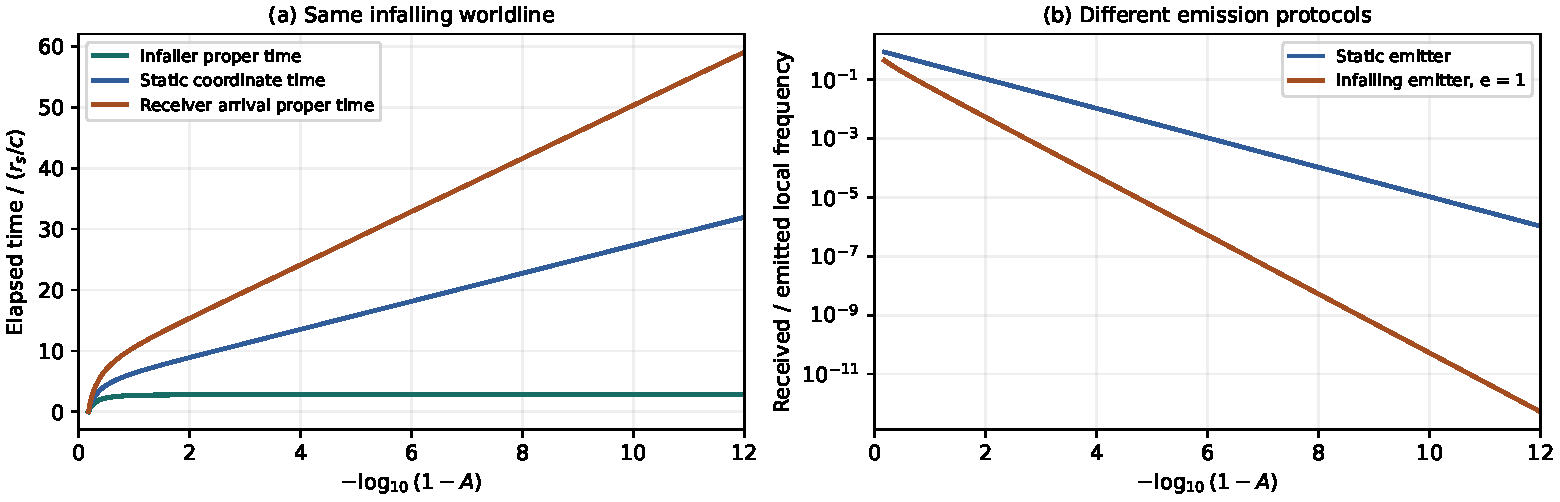
\includegraphics[width=.97\textwidth]{arrival_comparison.pdf}
\caption{Declared Schwarzschild benchmark, $r_i=3r_s$, radial geodesic
energy $e=1$, and an observer at $r_o=10r_s$. The horizontal variable is
$-\log_{10}(1-A)$, with the exact conversion to $r/r_s$ retained.
Left: elapsed infaller proper time approaches a finite limit while
static-coordinate and receiver-arrival times diverge. Each curve has
its initial value subtracted; times are in $r_s/c$. Right: gravitational
redshift for a static emitter and the full outgoing redshift for an
infalling emitter have different near-boundary powers. The latter
includes motion. These are mathematical controls, not trajectories or
measurements of a particular black hole.}
\label{fig:arrival}
\end{figure*}

\section{The original interacting clock remains an explicit input}
The geometry supplies a proper-time history only after a metric and
worldline have been selected. Applying the Chapter I clock then
requires the complete coupling and common calibration retained in
Chapter IV. Write $\zeta=E_u/I_u$ for the common conversion and
\begin{equation}
 \eta_j=\zeta(\tau_j-\tau_{j,0}),\qquad
 \theta_j=\theta_{l,0}(\eta_j).
\end{equation}
Under ideal phase encoding with known transfer phase, the rate of a
received source phase relative to the receiver's same-lane clock is
\begin{equation}
 \mathcal R_l=
 \frac{d\tau_E}{d\tau_O}
 \frac{\nu_{l,0}(\eta_E)}{\nu_{l,0}(\eta_O)}.
 \label{eq:strong-actual-clock}
\end{equation}
The first factor is the geometric frequency ratio derived above; the
second retains the interacting transient. An equal-coordinate-time or
arbitrarily late reception comparison does not remove it. The complete
Hamiltonian coupling is a stated physical hypothesis here, not a
consequence of the test-particle metric.

The inherited phase/current bounds apply only on their certified
internal-age interval, ending at one bare cycle
$T_0=573049\pi$. A finite remaining source proper time can lie inside
that interval only after the common unit conversion and preparation
epoch are checked. An arbitrarily late receiving observer need not
remain inside its own certified window. The geometrical arrival
asymptotics are therefore not a new all-time microscopic clock theorem.
If a finite source-age interval is certified and
$0\leq\nu_{l,0}\leq u_l$, its remaining phase satisfies
$|\Delta\theta_l|\leq u_l\zeta\Delta\tau_E$; stretching its reception
across unbounded observer time does not turn it into an unbounded
source history.

\section{An original-state finite-gap clock protocol}
\label{sec:original-clock-protocol}
The completed Chapter I clocks can already be carried through a declared
strong-field event map without replacing them by bare two-state oscillators.
The result is conditional on a precise ideal-probe law; finite-size geometry
and the remaining curved-field theorem are recorded separately.

\subsection{The unchanged clock and the stated coupling}
For every original lane $l=(a,b)$ retain the exact interacting hard-branch
superposition with soft vacuum, signed $D,C$, both tensor polarizations,
complete sixteen-state source, even energy and both shell counterterms.
Its actual current satisfies
\[
 z_l=\langle Z_l\rangle,\quad \theta_l=-\arg z_l,\qquad
 \dot z_l=-\ii\Delta z_l+2g_lw_l.
\]
The joint correlator $w_l$ remains. The inherited certificate gives, for
$0\le\eta\le T_0=573049\pi$,
\[
 \ell_l\le\nu_l(\eta)\le u_l,\qquad
 |z_l|\ge m_l=M_{l,-}-E_l(T_0)>999/1000.
\]
The hard-reference disk bounds the actual phase; it does not replace it by
$\Omega_l\eta$. With the original full joint Hamiltonian $H_0$, assume the
conditional point-clock law
\[
 \ii\frac{\dd\Psi}{\dd\tau}=s_0H_0\Psi,\qquad
 \eta=s_0\tau,\quad s_0=e_u/I_u.
\]
Its exact evolution is the unchanged $\Psi_0(\eta)$. Every Hamiltonian term
receives the same proper-time conversion. This is a stated moving-probe
coupling, not a completed covariant action for the extended source and field.

The source normalization can be checked on the original real $Q$ in its full
address-pair basis. With $Q_L=Q\otimes I$, $Q_R=I\otimes Q$,
$D=Q_L-Q_R$, $C=\ii SD$ and
$H_{\rm pair}=S+Q_L+Q_R+Q_LQ_R$,
\[
 \begin{gathered}
 Z_{\rm raw}=D-SD,\qquad
 [H_{\rm pair},Z_{\rm raw}]=-2Z_{\rm raw},\\
 D^2+C^2=D^2-(SD)^2=2D^2.
 \end{gathered}
\]
The two nonzero full-source matrices are the native R1 operands. The actual
clock equation still contains its field correlator and the four dark states.

\subsection{One shared conversion and an exact finite arrival map}
Write $\bar t=ct/r_s$, $\bar\tau=c\tau/r_s$ and $y=\sqrt{r/r_s}$.
Use one declared fixture for every lane and both experiments:
\[
 \begin{gathered}
 e=1,\quad y_0=5/4,\quad y_1=1001/1000,\\
 r_o/r_s=25/9,\quad \sqrt{F_o}=4/5,\qquad
 \zeta=s_0r_s/c=T_0/16.
 \end{gathered}
\]
This conversion is not fitted by lane. Prepare emitter and receiver clocks
at coordinate $t=0$. Hold one emitter at $r_0=25r_s/16$; let the other follow
the inward $e=1$ geodesic. Compare equal emitter proper ages,
\[
 \bar\tau_e(y)=\frac23(y_0^3-y^3),\qquad
 y_j=y_0-\frac j8(y_0-y_1),\quad j=0,\ldots,8.
\]
Use ideal tagged radial-null events. This specifies the causal timing
benchmark; a continuous physical phase encoder needs its own coupling,
nonzero received amplitude and transfer calibration.

The first flight and the two exact arrival maps are
\[
 D_0=\frac{175}{144}+\log\frac{256}{81},\qquad
 \frac{\eta_{o,S}}{T_0}=\frac{D_0}{20}+\frac{\bar\tau_e}{12},
\]
\[
 \begin{aligned}
 \bar t_{o,F}(y)={}&\frac{365}{96}+\frac{25}{9}
     -\left(\frac23y^3+y^2+2y\right)\\
   &+\log\frac{16}{81(y-1)^2},\qquad
 \frac{\eta_{o,F}}{T_0}=\frac{\bar t_{o,F}}{20}.
 \end{aligned}
\]
The emitted proper tick factors are
\[
 \begin{gathered}
 g_S=\frac34,\quad g_F(y)=\frac{1-1/y}{\sqrt{F_o}},\\
 g_F(y_0)=\frac14,\qquad g_F(y_1)=\frac5{4004}.
 \end{gathered}
\]
The final finite gap is $F_1=2001/1002001$. Directed exact evaluation gives
\[
 \begin{array}{c|c}
 \text{clock age}&\eta/T_0\ \text{at final emission/arrival}\\\hline
 \text{emitter, either experiment}&0.039588416625\\
 \text{held receiver}&0.171084858879245\ldots\\
 \text{falling-experiment receiver}&0.755042078465470\ldots
 \end{array}
\]
All prefixes remain inside the original certificate, including receiver age.
The phase-event relation uses the actual $\theta_l(\eta_e)$ and
$\theta_m(\eta_o)$. For a calibrated phase carrier its received phase-rate
ratio to the receiver's own clock is
\[
 g\,\frac{\nu_l(\eta_e)}{\nu_m(\eta_o)}.
\]
Both interacting transients survive. The same-source arrival-generator
contrast and the exact six-lane inverse lower-derivative matrix are the
native R2 operands; they do not evolve a replacement field or source.

\subsection{Preparation, shots, timing and unwrapping}
Measure $X_l=P_lDP_l/d_l$ and $Y_l=P_lCP_l/d_l$, extended by zero outside
the lane. Both have norm one and outcomes in $\{-1,0,1\}$; leakage outcomes
remain in the mean. Each quadrature at each event uses fresh original joint
preparations. No first readout disturbs a later clock or quadrature.
A joint preparation infidelity $p$ gives expectation bias at most$2\sqrt p$.
Its energy account is a separate apparatus requirement.

There are at most480 scalar means: six lanes, four emitter/receiver histories,
ten slots and two quadratures. Independent bounded repetitions within each
mean give
\[
 P(\text{any statistical miss})\le960e^{-nd_{\rm stat}^2/2}.
\]
Two sufficient designs have statistical error$1/200$ or$1/2000$;
preparation and readout biases are respectively$1/400$ or$1/4000$ each.
They require preparation infidelities at most$1/640000$ or$1/64000000$,
and$10^6$ or$10^8$ shots per scalar mean. Total independent copies are
$4.8\times10^8$ or$4.8\times10^{10}$. Both union bounds are below0.01.
These are sufficient instrument conditions, not achieved precision or
minimal counts.

If $d$ is the summed scalar error, the complex current disk has radius
less than$3d/2$. Its phase error is bounded by
\[
 \arcsin\frac{3d/2}{m_l}
 \le\frac{3d/2}{999/1000-3d/2}.
\]
Adding timing and transfer-phase allowances of$1/1000$ each in the coarse
design, or$1/4000$ each in the fine design, gives total phase allowances
$\beta=1/50$ or$1/400$ radians.

The finite padded range has$g_F\ge1/1000$. Fine emission-age uncertainty
at most$1/4000000$ in$\bar\tau_e$, plus residual propagation/receiver timing
uncertainty at most$1/4000$ in$\bar\tau_o$, yields
$\delta\bar\tau_o\le1/2000$. Together with a shared relative conversion
error at most$1/200000$, the actual rate bounds fit the fine timing phase
allowance. These requirements include geometry and trigger uncertainty;
precision arithmetic alone does not meet them.

The executable bounds prove that every sampled phase increment, including
preparation to first reception, plus$2\beta$ is below$3<\pi$. Continuous
unwrapping is consequently unique on the simultaneous confidence event.
An endpoint qubit phase is not a winding record; preparation, control and
reference payments remain in their own accounts.

For measured phase increments$\Delta\hat\theta_e,\Delta\hat\theta_o$,
the elapsed proper-time ratio has the interval
\[
 \begin{aligned}
 \frac{\Delta\tau_e}{\Delta\tau_o}\ge{}&
 \frac{(\Delta\hat\theta_e-2\beta)_+\ell_l}
      {(\Delta\hat\theta_o+2\beta)u_l},\\
 \frac{\Delta\tau_e}{\Delta\tau_o}\le{}&
 \frac{(\Delta\hat\theta_e+2\beta)u_l}
      {(\Delta\hat\theta_o-2\beta)_+\ell_l},
 \end{aligned}
\]
when the denominator lower bound is positive. The common conversion cancels.
This is a finite-window quantity. Instantaneous frequency requires a further
window/geometry bound. The planned coarse whole-window envelopes separate
held and falling histories in every lane: approximately$[0.40991,1.30632]$
versus$[0.04135,0.08385]$. The fine design separates all eight adjacent
windows as well. These are confidence-resolution guarantees, not acquired
data. The calculation pays$4\beta$ when allowing every possible noisy data
realization and then forming its$2\beta$ confidence interval.

\subsection{Static size and freely falling tidal geometry}
With the same$c_*=1$ calibration, the original shell has
$R_{\rm phys}/r_s<1.454\times10^{-6}$. A declared proper source/apparatus
tube$L/r_s=10^{-4}$ contains it. This does not truncate the infinite field.
For a static center$\rho_c=r_c/r_s$, put$\lambda=L/r_s$,
$\rho_-=\rho_c-\lambda>1$. The exact local bound is
\[
 \left|\log\frac{N}{N_c}\right|
 \le\frac{\lambda}{2\rho_-^2\sqrt{1-1/\rho_-}}.
\]
It is below$1/25000$ at launch and below$1/800$ for a held tube at the
falling endpoint. Static lapse variation grows as$L/(2r_s\sqrt F)$ toward
closure. The exact inward proper distance is
\[
 \ell_H/r_s=\sqrt{x(1+x)}+\operatorname{asinh}\sqrt x.
\]
A wholly exterior static ball must have$L<\ell_H$; this is a size condition,
not an infaller crossing theorem. No Chapter IV small-Plummer constant is
extrapolated to$F\to0$.

The orthonormal Schwarzschild curvature remains finite in the radial
freefall frame: a radial boost cancels through$\gamma^2-\sinh^2\alpha=1$.
The spatial scale$L^2r_s/r_1^3<10^{-8}$ measures local tidal metric variation,
but is not a completed finite-clock error estimate. For initially comoving
radial geodesic separation$J$, the exact first-variation equation and bounds
are
\[
 J''=\frac{c^2r_s}{r(\tau)^3}J,
\]
\[
 \cosh\!\left(\sqrt{\frac{c^2r_s}{r_0^3}}\Delta\tau\right)
 \le\frac J{J_0}\le
 \cosh\!\left(\sqrt{\frac{c^2r_s}{r_1^3}}\Delta\tau\right).
\]
The exact solution sharpens this comparison bracket. With $\rho=r/r_s=y^2$,
\[
 \frac{J}{J_0}=\frac15\left(\frac y{y_0}\right)^4+\frac{4y_0}{5y},
 \qquad J_{ss}=\rho^{-3}J.
\]
It has $J(0)=J_0$ and zero initial relative velocity. At the retained endpoints,
\[
 \frac{J_1}{J_0}-1=\frac{992802978755001}{12219238281250000}
 =0.08124917084876092\ldots.
\]
The strain is exactly about $8.1249\%$ within linear geodesic deviation.\cite{ch5review}
A bound original quantum clock is not an unbound geodesic congruence. Its
restoring/tidal coupling must be calculated; small metric variation alone
does not bound its long-time dynamics.

\subsection{A same-mass short-window bridge}
The preceding calibration has$r_s=T_0/16$ model lengths. The wave-boundary
fixture instead has$r_s=10^{10}$ model lengths; these are distinct fixtures.
A separate bridge uses$c=1$, $\zeta=10^{10}$ for all six original clocks,
\[
\begin{gathered}r_0/r_s=1+2\times10^{-6},\quad r_o=r_0+100,\\
 y_1=\sqrt{1+2\times10^{-6}}-10^{-8}.\end{gathered}
\]
Exact directed evaluation gives final emitter age$200.000398\ldots$,
first receiver age$70710.675539\ldots$, held final receiver age
$70911.175313\ldots$ and falling final receiver age
$355687.588344\ldots$, all below$T_0$. The endpoint tick factor is
$0.000698291817502\ldots$. A separately specified$\beta=10^{-4}$ design
separates the whole-window ratios in all six lanes; it requires$10^{12}$
shots for each of144 scalar means. These demanding counts are sufficient
apparatus conditions, not achieved data. This short-window bridge shares the
wave fixture's mass/unit choice without changing the source or silently
combining the two calibrations.

\subsection{Original whole-field localization}
The original field has infinite support. The preceding spatial-tail estimate at the long-fall tube $L_{\rm model}=\zeta/10000$ clipped to the complete positive-energy ceiling in every lane. The centered calculation below retains annihilation/source-shift cancellation before taking norms, evaluates larger apparatus scales, and carries both propagated current insertions. No finite tube deletes the exterior field.

\section{Centered localization of the original clock field}
\label{sec:centered-clock-localization}
The original source shift cancels the leading hard-field term before any
norm is taken.  Keeping this cancellation gives a useful spatial bound for
the actual Chapter I preparations.  This section retains their signed
couplings, all sixteen source states, both tensor polarizations, the hard
eigenbranches with soft vacuum, the full field and both shell counterterms.
The spatial quantity is the positive residual-energy receiver of Chapter IV;
its identification with curved canonical stress is a separate problem.

\subsection{A first form moment suffices}
Write $K=\|T_g\Psi\|^2$, where
\[
 \begin{gathered}
 (T_g\Psi)_\alpha(k)=\sqrt{k}\,a_\alpha(k)\Psi
       -\frac{g u_R(k)}{\sqrt{k}}\sigma_\alpha\Psi,\\
 u_R(k)=\sqrt{\frac{2k}{\kappa\pi}}j_2(kR),\qquad\kappa=4/5.
 \end{gathered}
\]
Here $\epsilon=\Delta/2$, $S$ is the original swap/involution (the active
lane's remaining Pauli direction), and
\[
 \mu=\int_0^\infty u_R(k)^2/k\,\dd k
       =\frac{1}{5\kappa R}=\frac{1}{4R},\qquad
 C_{\rm ct}=2g^2\mu.
\]
The source's full even block energy is retained. It commutes with the
lane-preserving field receiver and cancels in same-lane comparisons.
For an original hard branch $\Phi_j$, let $B_j=H_h-E_j\ge-\Delta$ and
$v=\sigma_\alpha\Phi_j$.  At the original split $\lambda=64\Delta$,
pull-through gives the centered expression
\[
 (T_g\Phi_j)_\alpha(k)
 =-\frac{g u_R(k)}{\sqrt{k}}B_j(B_j+k)^{-1}v,
 \qquad k\ge\lambda.
\]
All these spectral statements hold in the original invariant unordered-pair
source block containing $\Phi_j$ and $\sigma_\alpha\Phi_j$. Other source
blocks and dark states remain orthogonal retained sectors; their even
energies are not covered by this same-lane spectral gap.
No vector $B_jv$ is assumed.  Spectral calculus instead gives
\[
 \|B_j(B_j+k)^{-1}v\|^2
 \le\frac{\langle v,(B_j)_+v\rangle}{4k}
       +\frac{\Delta^2\|v\|^2}{(k-\Delta)^2}.
\]
The positive part follows from $b^2/(b+k)^2\le b/(4k)$ for $b\ge0$;
the negative part uses $-\Delta\le b<0$.  These are form-domain statements.

Peel off the two retained low hard branches, using their original isolated
two-branch gap certificate.  If $Q_h$ is their orthogonal complement, then
$Q_h B_jQ_h\ge0$ and
\[
 \|Q_h\sigma_\alpha\Phi_j\|^2\le1-M_-^2.
\]
Set $b_2=\int u_R^2/k^2\le5/72$, $h=64/63$,
$n_+={2g^2b_2h^2}/{(1+2g^2b_2h^2)}$ and
\[
 F_*=4|g|\sqrt{\mu}\bigl(\sqrt{C_{\rm ct}}+\sqrt{2K_{\rm prep}}\bigr).
\]
The actual source-conjugation identity, the hard-branch source charge and
the certified $0<\Omega\le\Delta$ give positive first form moments
\[
 \begin{split}
 M_{Q,0}&\le F_*+\Delta-\Omega_-M_-^2,\\
 M_{Q,1}&\le F_*+2\Delta n_+.
 \end{split}
\]
Nonnegative upper ceilings are used if an interval endpoint needs them.
The exact full-source check is
$DH_{\rm pair}D-D^2H_{\rm pair}=-2SD^2$;
the field contribution keeps the other polarization.  Thus this is a
source-bound first-moment estimate, without an ultraviolet operator moment.
The new centered whole-energy ceiling is intersected with the stronger
inherited $K_{\rm prep}$ whenever appropriate.  It improves lanes
$01,02,12$; no uniform improvement is claimed for the other three lanes.

\subsection{Spatial tails and both instantaneous insertions}
Use the original regular Bessel/TT isometry $J$ and radial split at $L$:
$K_{\rm out}[\Psi]=\|1_{r>L}JT_g\Psi\|^2$.
For the centered hard amplitude, split the Bessel integral at $k_0=1/R$,
integrate each oscillatory term once by parts, and keep its endpoint at
$\lambda$.  On the positive complement use either its norm ceiling or its
first form moment, taking the better valid bound for each integral.
The complete nine high-frequency Bessel products and the entire soft shift
are retained.  Explicit coefficients and directed arithmetic are in the
accompanying derivation and executable certificate.

Source charge makes the radial square form diagonal between the original
two hard branches.  Low-branch and complementary spectral amplitudes are
also orthogonal.  Their squares therefore add before the remaining
hard/soft triangle inequality.  The fully coupled original flat evolution
then obeys
\[
 \begin{split}
 \eta(T,L)&\le\min\{\mathcal K_*,D_K(T,L)^2\},\\
 D_K(T,L)&=\sqrt{p_{\rm out,prep}(L)}
       +\sqrt{2(1+C_{\rm ct})d_A^2(T)},\\
 \mathcal K_*&=K_{\rm prep}+\epsilon E(T),\\
 d_A^2(T)&\le8T^2g^2v_{\rm soft}
    \left[1+\bigl(\sqrt{C_{\rm ct}}+\sqrt{\mathcal K_*}\bigr)^2+\lambda\right].
 \end{split}
\]
Here $E(T)\le(T/T_0)^2E(T_0)$ for $T\le T_0$.
The hard/free-soft comparison generator includes the retained soft
counterterm, so its global reference phase is matched in the vector-distance
estimate.
No field is truncated at the displayed radius.  Over the complete original
window $T_0=573049\pi$, the certified tail fractions are
\begin{center}
\begin{tabular}{c|ccc}
lane & $L=T_0/160000$ & $L=10^4$ & $L=10^6$\\\hline
01&1&0.0234440&0.000262687\\
02&1&0.0232842&0.000246210\\
03&1&0.0340807&0.000342323\\
12&1&0.0234231&0.000260502\\
13&1&0.0340646&0.000342224\\
23&1&0.0340450&0.000342101
\end{tabular}
\end{center}
The entries are upper ceilings, not measured fractions or tail lower
bounds.  The first radius is about $11.25$ in the original model chart;
there the certificate still clips at the whole energy.  At $10^6$ it no
longer does so.

For $Z=\sigma_z+\mathrm{i}\sigma_y$ and its adjoint, the exact identity
$T_\alpha Z=ZT_\alpha-g(u_R/\sqrt{k})[\sigma_\alpha,Z]$ gives
\[
 \sqrt{K_{\rm out}[Z\Psi]},\ 
 \sqrt{K_{\rm out}[Z^\dagger\Psi]}
 \le2\sqrt{K_{\rm out}[\Psi]}
       +\sqrt{8/5}\,\frac{C_F(L)}{L^{5/2}},
\]
where $\|F_\alpha(r)\|\le C_F(L)/r^4$ is the complete shell shift.
This is an instantaneous bound.  It does not identify the tails of
backward-propagated insertions with instantaneous tails.

\subsection{A finite current disk with propagated insertions}
There is a finite comparison which needs only a global form ceiling for
the propagated insertions.  Specify the receiving Hamiltonian
\[
 H_W=\epsilon S+T_g^*WT_g,\qquad
 m_W I\le W\le M_W I,\quad m_W>0,
\]
with time-independent $W$ on the common closed form domain
$\mathcal Q=D(H_f^{1/2})$. The field receiver is the identity on source
blocks. The common even source energy is
retained and cancels from this comparison.  Let the difference form obey
\[
 |r[\Phi,\Psi]|\le\varepsilon_{\rm near}
       \sqrt{K_{\rm in}[\Phi]K_{\rm in}[\Psi]}
       +B_{\rm far}\sqrt{K_{\rm out}[\Phi]K_{\rm out}[\Psi]}.
\]
Put the perturbed backward observable
$O_W(t)=U_W(T-t)^\dagger ZU_W(T-t)$ against the \emph{original}
reference state $\Psi_0(t)$.  Energy conservation, form coercivity and
$K[Z\xi],K[Z^\dagger\xi]\le4(\sqrt{K[\xi]}+\sqrt{C_{\rm ct}}\|\xi\|)^2$
give, for both insertions,
\[
 \begin{split}
 K[O_W(t)\Psi_0(t)]&\le K_B,\\
 K[O_W(t)^\dagger\Psi_0(t)]&\le K_B,\\
 K_B&=\frac{4M_W}{m_W}
  \left(\sqrt{\frac{M_W\mathcal K_*+2\epsilon}{m_W}}+\sqrt{C_{\rm ct}}\right)^2
       +\frac{8\epsilon}{m_W}.
 \end{split}
\]
The weak Heisenberg identity now yields the finite, nonperturbative disk
\[
 \begin{gathered}
 |z_W(T)-z_0(T)|\le\mathcal E_z,\\
 \mathcal E_z=2T\sqrt{K_B}\left(
    \varepsilon_{\rm near}\sqrt{\mathcal K_*}
       +B_{\rm far}\sqrt{\eta(T,L)}\right).
 \end{gathered}
\]
Both $O_W$ and $O_W^\dagger$ occur in its commutator.  No unknown
perturbed-state spatial tail has been replaced by a reference tail.
If $|z_0|\ge a_*>\mathcal E_z$, the continuous unwrapped phase error is
at most $\arcsin(\mathcal E_z/a_*)$.

For one explicit smooth bounded assay, take
\[
 N_L(r)=1+10^{-3}+(1/2-10^{-3})\,
             \chi\!\left(\frac{r-L}{L}\right),\qquad W=J^*N_LJ,
\]
where $\chi(s)=0$ for $s\le0$, $\chi(s)=1$ for $s\ge1$, and in between
$\chi(s)=e^{-1/s}/(e^{-1/s}+e^{-1/(1-s)})$.
This specifies the entire profile, including the exterior.
Use the conservative class $m_W=1/2,M_W=3/2$,
$\varepsilon_{\rm near}=10^{-3},B_{\rm far}=1/2$, $L=10^6$.
For the retained same-mass bridge, all model ages are below $T=355689$.
The six phase-error upper bounds are
\[
 \begin{array}{c|r}
 l& |\delta\theta_l|\text{ upper bound}\\\hline
 01&3.421\,10^{-7}\\
 02&1.533\,10^{-6}\\
 03&4.911\,10^{-4}\\
 12&3.945\,10^{-7}\\
 13&4.434\,10^{-4}\\
 23&3.957\,10^{-4}
 \end{array}
\]
in radians, each below $10^{-3}$.  The largest current disk is below
$4.908\,10^{-4}$.  At the full $T_0$, the largest phase bound is below
$2.495\,10^{-3}$ instead.  These are actual-original-state results for
the stated positive receiver, with the original interacting transient.

\subsection{The remaining physical obstruction is quantitative}
The assay above is not the full Schwarzschild lapse or a curved canonical
Hamiltonian.  In the same-mass geometry, $r_s=10^{10}$,
$r_0/r_s=1+2\,10^{-6}$, the radius $L=10^6$ remains smaller than a
rigorous endpoint proper distance to the horizon, $2.8142\,10^7$.
Nevertheless the normalized static lapse has near variation bounded by
$0.035534$, far contrast exceeding $706$, and global infimum zero.
Thus it fails the displayed coercivity class.  Even optimistically keeping
that class's constants, lane $03$ at the short window would need a
far-tail fraction below approximately $8.72\,10^{-10}$ if its near error
were zero; the present upper certificate is about $3.41\,10^{-4}$.
This comparison describes a gap in the proof, not a lower bound on the
actual physical error.

A curved canonical completion must additionally control its pair kernel,
vacuum convention, source-shell vertices/counterterms and all angular
complement returns on the original state and its propagated insertions.
The tempting direct equation for $T_gU_0(t)$ contains
$[H_0,\sigma_\alpha]$ and the shell field $\phi(u_R)$.
Here $u_R\notin L^2$ although $u_R/\sqrt{k}\in L^2$; its Hilbert-space
commutator norm cannot be assumed from finite $K$ alone.
The first-form method avoids that unavailable norm and the finite receiver
theorem avoids propagating an instantaneous spatial estimate as though it
were a two-time estimate.  Neither step supplies the still missing curved
joint propagator.


\section{A critical curve is not a photograph of the boundary}
For a static observer at $r_o$ in a spherical metric, a local orthonormal
measurement of a null ray gives
\begin{equation}
 \sin\alpha=\frac{b\sqrt{F_o}}{r_o}.
 \label{eq:finite-shadow-angle}
\end{equation}
Indeed the local photon energy is the conserved Killing energy divided
by $\sqrt{F_o}$, whereas its transverse momentum is its angular
momentum divided by $r_o$. Their ratio yields the displayed angle.
For an exterior observer $r_o>r_{\rm ph}$ in the Schwarzschild
black-hole benchmark, the critical-cone angle uses
$b=b_{\rm crit}$ and the appropriate inward sky branch. At large
$r_o$, its angular diameter approaches $2b_{\rm crit}/r_o$.

The areal photon-sphere radius, the impact-parameter critical curve,
and the observed emission ring are different objects. A dark capture
region additionally needs an absorbing/global completion and a specified
illumination model. Emission, absorption, lensing, source motion,
polarization and instrument response determine the bright image.
The 2019 EHT mass inference calibrates an observed emission diameter
against a model family; it is not a direct measurement of material
crossing $A=1$.\cite{eht,gralla}

A no-completed-crossing model must therefore supply its boundary
response: absorption, reflection, re-emission or another causal rule,
with energy and record transfer retained. Agreement with the exterior
photon-sphere scale alone cannot select among these possibilities.
If a proposed surface lies at $r_b=r_s(1+\epsilon)$ and an exterior
reflecting/scattering region is represented at $r_p>r_b$, the benchmark
radial round-trip interval between them is
\begin{equation}
 \Delta t_{\rm rt}=\frac2c\left[r_*(r_p)-r_*(r_b)\right]
 =-2t_s\log\epsilon+O(1).
\end{equation}
This conditional time scale is not an echo prediction. It says nothing
about excitation, reflection amplitude, wave potential, attenuation or
detector observability until those are specified. A prescribed
boundary that absorbs all relevant signals need not produce such a
return, and a wave-scattering peak is not automatically a physical
mirror.


\subsection{A declared tensor-mode wave and boundary law}
The retained carrier has both original signed tensor polarizations, the
whole-sphere TT-image isometry, the full positive channel metric
$\kappa=2B/5$, and driven angular eigenvalue six. Its tensor block has
$\kappa=4/5$. A curved propagation equation needs a further choice.
We make \emph{hypothesis RM}: on the prescribed static spherical metric,
retain the original mode space and nonnegative angular operator
$\mathcal L$, self-adjoint and nonnegative in the $\kappa$ inner product
(or commuting with $\kappa$ in the ordinary convention), and choose
\begin{equation}
\begin{split}
 S_{\rm RM}=\frac14\int dt\,dr\,\bigg[
 &\frac{r^2\sqrt H}{Nc^2}\phi_t^*\kappa\phi_t
 -\frac{r^2N}{\sqrt H}\phi_r^*\kappa\phi_r\\
 &-N\sqrt H\,\phi^*\kappa\mathcal L\phi\bigg],\qquad N=\sqrt F.
\end{split}
\label{eq:wp-RM}
\end{equation}
At $F=H=1$ this is the original radial tensor action. RM is a stated
extension of those mode amplitudes, with their original tensor incidence;
it does not select a unique covariant spin-two theory. A curvature coupling,
spin connection or constrained field completion would require its own
derivation. No scalar carrier or general-relativistic perturbation
potential is silently substituted.

Set $dx/dr=\sqrt{H/F}$, $a=dr/dx=\sqrt{F/H}$ and $u=r\phi$.
Variation and a radial integration by parts give
\begin{equation}
 \frac{u_{tt}}{c^2}-u_{xx}+Vu=0,\qquad
 V=\frac{F\mathcal L}{r^2}+\frac{(F/H)'}{2r}I.
 \label{eq:wp-potential}
\end{equation}
Nonnegative $\mathcal L$ does not alone make $V$ nonnegative on an arbitrary metric:
$(F/H)'/(2r)$ can be negative. The complete coercive form and surface terms
must be checked there. The driven quadrupole of the Schwarzschild comparison has
$V=F(6/r^2+r_s/r^3)$. The other angular and channel directions remain;
RM's spherical coefficients preserve their sectors. An added angular
coupling must propagate its full complement and possible return.

The surface term is part of the energy. With real parts and both
polarizations understood,
\begin{equation}
\begin{gathered}
 E_u=\frac\kappa4\int\left(\frac{|u_t|^2}{c^2}
                 +|u_x|^2+u^*Vu\right)dx,\\
 E_\phi=E_u-\frac\kappa4
       \left[\frac ar|u|^2\right]_{b}^{p},\\
 j_\phi=-\frac\kappa2\operatorname{Re}(u_t^*u_x)
       +\frac\kappa4\partial_t\left(\frac ar|u|^2\right).
\end{gathered}
\label{eq:wp-surface}
\end{equation}
These identities preserve the original $1/4$ action normalization.

\subsection{Passive termination, physical storage and causal response}
At $x_b=0$ choose the explicit termination
\begin{equation}
 u_x=\frac{u_t+\sigma u}{c},\qquad \sigma>0.
 \label{eq:wp-boundary}
\end{equation}
Its canonical spring energy is $E_s=\kappa\sigma|u_b|^2/(4c)$ and
its absorbed power is $P_d=\kappa|u_{b,t}|^2/(2c)$. In the original
field variables the physical spring and outer-port storage are
\begin{equation}
\begin{gathered}
 E_{s,\phi}=\frac\kappa4
       \left(\frac\sigma c-\frac{a_b}{r_b}\right)|u_b|^2,
 \qquad E_{\rm port}=\frac{\kappa a_p}{4r_p}|u_p|^2,\\
 E_\phi+E_{s,\phi}+E_{\rm port}=E_u+E_s.
\end{gathered}
\label{eq:wp-paid-spring}
\end{equation}
Thus the physical spring is positive when $\sigma>ca_b/r_b$.
For a characteristic matched launch/readout port at $x_p=L$, write
$u_p=u_{\rm in}+u_{\rm out}$ and impose
$u_t+cu_x=2u_{{\rm in},t}$. The complete balance is
\begin{equation}
 \frac d{dt}(E_\phi+E_{s,\phi}+E_{\rm port})+P_d
 =\frac\kappa{2c}
    (|u_{{\rm in},t}|^2-|u_{{\rm out},t}|^2).
 \label{eq:wp-energy}
\end{equation}
Incoming fields add their full energies and interference terms. The port
retains the exterior recipient; it does not declare the actual spacetime
outside $r_p$ free of scattering.

For zero potential the boundary reflection is exactly
\begin{equation}
\begin{gathered}
 R(s)=-\frac\sigma{2s+\sigma},\\
 (Rf)(t)=-\frac\sigma2\int_{-\infty}^t
            e^{-\sigma(t-v)/2}f(v)\,dv.
\end{gathered}
\label{eq:wp-transfer}
\end{equation}
Its pole is stable, the response is causal, its impulse-response $L^1$
norm is one and $|R(i\omega)|\leq1$. A return therefore has an amplitude,
a storage history and an exponential tail, in addition to delay $2L/c$.
This is a selected boundary law, not a thermal-state assertion.

\subsection{A complete original-pulse finite-gap experiment}
Use the original maintained compact pulse, both signed polarizations,
all six $g_{ab}$ and radius balls, $\Delta=2/573049$, and $c=c_*=1$
in the shared model chart. With $z=\Delta R$ and
$\mu(w)=15(1-w^2)^2/16$ on $[-1,1]$, the complete original carrier is
\begin{equation}
\begin{gathered}
 F_p(v)=\sin^4(v/8)e^{-iv},\quad0\leq v\leq8\pi,\\
 \psi_{\rm original}(t)=A_0 C_zF_p''(\Delta t),\qquad
 A_0=\frac{2g_{ab}z^2}{15\kappa},\\
 C_zh(v)=\int_{-1}^1\mu(w)h(v-zw)\,dw.
\end{gathered}
\label{eq:wp-original}
\end{equation}
$F_p$ is zero outside its stated support. This exact positive averaging
retains both compact edges. Its original energy deficit relative to the
small-source value is below $6.633\times10^{-14}$.

The launcher subsystem retains the original source even energy, full
local field, drive $-\operatorname{Re}(f^*\phi(R))$ and counterterm
$|f|^2/(4R)$. At a uniform local lapse $N_p$, the whole subsystem and
its switching ledger scale by $N_p$. The calibrated isometric launch
$u_{\rm in}(t)=\psi_{\rm original}(N_pt)$ then supplies Killing energy
$E_{\rm in}=N_pW_{\rm original}$. This is a declared composite maintained
experiment, not a microscopic central source placed within the macroscopic
$r_s$, nor an autonomous four-cycle quantum-clock certificate.
Finite launcher size requires the separate worldtube error bound.

A genuinely nonuniform central-shell coupling would instead require
the full curved static inverse: if its free form is
$\langle\phi,A\phi\rangle/4$ and its drive is
$-\langle j,\phi\rangle$, completing the square requires
$H_{\rm ct}=\langle j,A^{-1}j\rangle$, when that source functional has
a finite inverse-form value. The flat quadrupole gives
$1/(5\kappa R)$ and recovers the original counterterm. It is not generally
correct to retain that numerical coefficient after changing the entire
radial geometry.

Choose one finite gap and boundary rate before evaluating the pulse:
\begin{equation}
\begin{gathered}
 r_s=10^{10},\quad\delta=10^{-6},\quad
 r_b=r_s(1+\delta),\quad r_p=r_s(1+2\delta),\\
 N_p^2=\frac1{500001},\quad\sigma=N_p\Delta,\quad
 L=r_s(\delta+\log2),\\
 0\leq V\leq V_{\max}=\frac{14\delta}{r_s^2}.
\end{gathered}
\label{eq:wp-gap}
\end{equation}
The microscopic source radius remains approximately $0.163544$ in this
chart. Here $\sigma\simeq4.935746\times10^{-9}$, whereas
$a_b/r_b\simeq10^{-16}$; the original-variable spring is strictly positive.
No SI calibration is inferred from the selected model lengths.

For the zero-potential response to $F_p''$, its exact five frequencies
are $\omega=(1/2,3/4,1,5/4,3/2)$, with
$c=(1/16,-1/4,3/8,-1/4,1/16)$. On $[0,U]$, $U=8\pi$,
\begin{equation}
\begin{gathered}
 H(v)=\sum_jh_je^{-i\omega_jv}-S e^{-v/2},\\
 h_j=\frac{\omega_j^2c_j}{1-2i\omega_j},\quad S=\sum_jh_j,\\
 H(v)=S(1-e^{-4\pi})e^{-(v-U)/2},\quad v>U.
\end{gathered}
\label{eq:wp-pulse-return}
\end{equation}
The initial transient and final tail are required by the compact pulse.
Direct integration gives
\begin{equation}
\begin{gathered}
 I_{\rm in}=\int|F_p'''|^2dv=\frac{14245\pi}{4096},\\
 I_{\rm ret}=\int|H'|^2dv
 =\frac{2128297\pi}{3860480}
   -\frac{243(1-e^{-4\pi})}{5821603840}.
\end{gathered}
\label{eq:wp-energy-coefficients}
\end{equation}
Thus $I_{\rm ret}/I_{\rm in}=0.1585215864253203$ and the absorbed
fraction is $0.8414784135746797$. Positive source smoothing changes this
fraction by less than $10^{-13}$. These are exact-pulse boundary-model
results, not a monochromatic approximation.

\paragraph{The nonzero potential and every further return.}
Let $G_0$ be the free retarded Green kernel with the stated passive
termination and matched outer port. The complete potential is retained by
\begin{equation}
 u=u_0-c^2\int_0^t\!\int_0^L
       G_0(t-s;x,y)V(y)u(s,y)\,dy\,ds.
 \label{eq:wp-Volterra}
\end{equation}
The direct kernel plus its causal reflected image obeys $|G_0|\leq1/c$.
For $B=17|A_0|/16$, define the exact positive integrated potential
\[
 J_V=6\left(\frac1{r_b}-\frac1{r_p}\right)
 +\frac{r_s}{2}\left(\frac1{r_b^2}-\frac1{r_p^2}\right),
 \qquad q=cJ_VT.
\]
The complete Volterra equation uses this $L^1$ norm. Gronwall and differentiated
delayed kernels yield
\begin{equation}
\begin{gathered}
 \|u-u_0\|_\infty\leq2B(e^q-1),\\
 \|u_t-u_{0,t}\|_\infty\leq2cJ_VB e^q,\qquad
 \|u_x-u_{0,x}\|_\infty\leq2J_VB e^q.
\end{gathered}
\label{eq:wp-errors}
\end{equation}
The exact original compact edges satisfy the weak-derivative requirements.
Potential backscatter can arrive before the inner-boundary round trip;
that earlier response is not a signal launched from the inner boundary.

Take $T=(8\pi+2z_{\max}+32)/\sigma+2L/c$. The interval certificate gives
$q<1.781\times10^{-5}$, returned-waveform error below
$3.784\times10^{-5}|A_0|$, and finite-window returned-energy error below
$8.226\times10^{-6}E_{{\rm in},0}$. It also retains the entire late
field, potential, physical spring and port storage:
$(E_u(T)+E_s(T))/E_{{\rm in},0}<6.582\times10^{-11}$.
Passivity bounds any later returned energy by this residual. The all-time lower
energy endpoint also subtracts the free reference pulse's post-window tail;
a sufficient allowance is $6.756\times10^{-23}E_{{\rm in},0}$.\cite{ch5review} After also
normalizing to the true smoothed input, all six preparations satisfy
\begin{equation}
 0.15851336\leq\frac{E_{\rm ret}}{E_{\rm in}}\leq0.15852982.
 \label{eq:wp-final-return}
\end{equation}
The amplitudes below retain their original signs; the incident energies use the common model normalization;
each preparation has weight $1/6$.
\begin{center}
\small
\begin{tabular}{rcc}
\hline
pair & signed $A_0$ & $E_{{\rm in},0}$\\\hline
01 & $-5.18100\,10^{-18}$ & $5.79019\,10^{-43}$\\
02 & $-1.07380\,10^{-17}$ & $2.48723\,10^{-42}$\\
03 & $-1.33669\,10^{-16}$ & $3.85414\,10^{-40}$\\
12 & $-5.55704\,10^{-18}$ & $6.66119\,10^{-43}$\\
13 & $-1.28488\,10^{-16}$ & $3.56116\,10^{-40}$\\
23 & $-1.22931\,10^{-16}$ & $3.25978\,10^{-40}$\\\hline
\end{tabular}
\end{center}
The exact input balls and outward intervals are retained in the replay.
Absorbed plus returned energy equals incident energy after the residual
leaves or dissipates. During the experiment the residual stays in the
ledger. The launcher pays the original maintained-source work and
switching payments; zero net counterterm endpoint change does not establish
zero apparatus cost.

The decay limit also has a short certificate for this regular finite
interval. A nonzero-frequency undamped mode has zero damping at the matched
port, hence $u(L)=u_x(L)=0$ and is identically zero. A static mode obeys
$\int(|u_x|^2+V|u|^2)dx+(\sigma/c)|u(0)|^2=0$, so it too vanishes.
The smooth compact input leaves a precompact energy orbit under the
contractive evolution; its invariant limit is therefore zero. No numerical
decay rate is assumed in the finite-time residual bound above.

\subsection{Static and infalling escape cones}
For isotropic emission by a static source at $r_s<r<3r_s/2$ in the
comparison geometry,
\begin{equation}
 \sin\alpha_c=\frac{b_{\rm crit}\sqrt F}{r},\qquad
 f_{\rm esc,stat}=\frac{1-\cos\alpha_c}{2}
                   \sim\frac{27F}{16}.
 \label{eq:wp-escape-static}
\end{equation}
The fraction counts all $4\pi$ directions; an outward-hemisphere
normalization doubles it. For steady emission the total escaped power at
a complete outer static sphere has the further energy/rate factor $F/F_o$.
Finite pulses need their angular travel-time distribution.

For inward geodesic emission let $\beta=\sqrt{1-F/e^2}$ and
$\mu'=\cos\alpha'$ in the emitter's rest frame. Aberration and energy
conversion give
\begin{equation}
\begin{gathered}
 \mu=\frac{\mu'-\beta}{1-\beta\mu'},\qquad
 \frac{E_o}{E_{\rm em}}=\frac{e(1-\beta\mu')}{\sqrt{F_o}},\\
 \mu'_c=\frac{\mu_c+\beta}{1+\beta\mu_c},\qquad
 f_{\rm esc,fall}=\frac{1-\mu'_c}{2}
                    \sim\frac{27F^2}{64e^2}.
\end{gathered}
\label{eq:wp-escape-fall}
\end{equation}
The radial ray recovers the earlier infaller redshift. A total received
luminosity additionally needs emission, angular acceptance and the
angle-dependent event maps; the radial factor alone does not supply it.


% Owner-review §§6--9, independently verified; no predecessor source edits.
\subsection{The static inverse with the actual apparatus endpoints}
The supplied review gives a useful closed inverse for hypothesis RM.
Its endpoint choice must agree with the physical question. For a
Schwarzschild angular sector,
\begin{equation}
 A_l=\kappa\left[-\partial_r r(r-r_s)\partial_r+l(l+1)\right].
 \label{eq:li-static-A}
\end{equation}
Here angular positivity is in the $\kappa$ inner product; alternatively
conjugate by $\kappa^{1/2}$. On an arbitrary metric it does not alone
imply positivity of the transformed $V$, whose radial term can have either
sign. The original complete form and its surface terms control that issue.
The selected Schwarzschild annulus is positive and regular.

For the actual finite experiment, retain the inner spring and the
zero-input static limit of the matched outer port:
\begin{equation}
\begin{gathered}
 u_x(r_b)=\frac\sigma c u(r_b),\qquad u_x(r_p)=0,\\
 \mathcal B_bh=F_b(h+r_bh')-\frac{\sigma r_b}{c}h,
 \qquad \mathcal B_ph=F_p(h+r_ph').
\end{gathered}
\label{eq:li-static-BC}
\end{equation}
The positive original-field spring and outer-port storage remain in this
domain. On the finite interval the complete form controls $H^1$ and its
trace evaluations, so the source inverse-form value is finite.

Put $y=2r/r_s-1$. For $l=2$,
\begin{equation}
 P=\frac{3y^2-1}{2},\qquad
 Q=\frac P2\log\frac{y+1}{y-1}-\frac{3y}{2}.
\end{equation}
Their Wronskian obeys
$r(r-r_s)(PQ'-P'Q)=-r_s/2$. Define
$v_b=P\mathcal B_bQ-Q\mathcal B_bP$ and
$v_p=P\mathcal B_pQ-Q\mathcal B_pP$. Then
\begin{equation}
\begin{gathered}
 C=-r(r-r_s)(v_bv_p'-v_b'v_p)>0,\\
 G_l(r,r')=\frac{v_b(r_<)v_p(r_>)}{\kappa C},\\
 G_\phi(r_p,r_p)=
 \frac{v_b(r_p)}{\kappa r_pF_p[v_b(r_p)+r_pv_b'(r_p)]}.
\end{gathered}
\label{eq:li-finite-G}
\end{equation}
The jump is $r(r-r_s)[G_r^+-G_r^-]=-1/\kappa$.
The complete positive form establishes the inverse and excludes a zero
denominator; the Wronskian sets its normalization.

For the unchanged $r_s,r_b,r_p,\sigma$ of the pulse experiment,
outward rational logarithm and square-root intervals give
\begin{center}
\small
\begin{tabular}{p{.61\columnwidth}r}
\hline
Source and endpoints & $G_\phi$\\\hline
Actual outer port, finite apparatus
 & $8.91755323\,10^{-11}$\\
Areal test shell $r_a=(r_b+r_p)/2$, same apparatus
 & $5.32154769\,10^{-11}$\\
Same $r_a$, horizon regular and infinity decaying
 & $1.30128154\,10^{-9}$\\\hline
\end{tabular}
\end{center}
The areal test shell is not the microscopic off-center launcher's radius
$R$. The original local $1/(4R)$ counterterm therefore remains distinct.
For a source drive $-\operatorname{Re}(f^*\phi)$ with free form
$\langle\phi,A\phi\rangle/4$, square completion requires
$H_{\rm ct}=|f|^2G_\phi$. Here $G$ is the inverse-form kernel; the physical static minimizer is $\phi=2Gf$. The actual incoming characteristic gives the
effective port force $j_u=\kappa u_{{\rm in},t}/c$, or
$f_\phi=r_pj_u$; it does not identify the microscopic $g_{ab}$ with
a macroscopic static force. Promoting this controlled port force to a
Hamiltonian source requires its own counterterm and paid preparation.
A prepared incoming guide state's energy is already in the full guide
Hamiltonian and is not charged twice.

Angular mixing requires the complete inverse. In block notation its
retained block is
$(A_{PP}-A_{PQ}A_{QQ}^{-1}A_{QP})^{-1}$, which can exceed
$A_{PP}^{-1}$. Discarding the complement can remove a positive return.

The separately declared horizon-regular/infinity-decaying kernel is
$2P_l(y_<)Q_l(y_>)/(\kappa r_s)$. At fixed central areal radius its flat
limit is $1/[\kappa(2l+1)r_a]$, and for $l=2$ its near-boundary diagonal
is $[\log(r_s/(r_a-r_s))-3+o(1)]/(\kappa r_s)$.
The actual finite apparatus has a different flat limit: hold its radii and
$\sigma$ fixed, send $r_s\to0$ and use the same Robin conditions on
$r^l,r^{-l-1}$. Its outer-port limit is
$2.53265981\times10^{-12}$. The domain, rather than a coordinate label,
selects the counterterm.

\subsection{The exact integrated potential sharpens the unchanged pulse}
The supplied review observes that the complete causal proof needs
$\int Vdx$, rather than $V_{\max}L$. For the actual quadrupole,
\begin{equation}
 J_V=6\left(\frac1{r_b}-\frac1{r_p}\right)
       +\frac{r_s}{2}\left(\frac1{r_b^2}-\frac1{r_p^2}\right).
 \label{eq:li-JV}
\end{equation}
With $B=17|A_0|/16$, the same exact Volterra equation implies
\begin{equation}
\begin{gathered}
 \|u-u_0\|_\infty\leq2B(e^{cJ_VT}-1),\\
 \|u_t-u_{0,t}\|_\infty\leq2cJ_VBe^{cJ_VT},\qquad
 \|u_x-u_{0,x}\|_\infty\leq2J_VBe^{cJ_VT}.
\end{gathered}
\end{equation}
Use $J_V$ in the residual potential energy too. Every scattering order,
both compact edges and all six original signed amplitudes/radius balls
remain. For the unchanged final time the resulting ceilings are
\begin{center}
\small
\begin{tabular}{lr}
\hline
Quantity & Bound\\\hline
$cJ_VT$ & $1.780673\,10^{-5}$\\
Waveform error$/|A_0|$ & $3.783964\,10^{-5}$\\
Finite-window energy error$/E_{{\rm in},0}$ & $8.225496\,10^{-6}$\\
Late field/spring/port energy$/E_{{\rm in},0}$ & $6.581033\,10^{-11}$\\
Free post-window return tail$/E_{{\rm in},0}$ & $6.755624\,10^{-23}$\\\hline
\end{tabular}
\end{center}
The last positive term must be subtracted from a finite-window lower
comparison to the reference's all-time returned energy. Applying source
smoothing and normalizing every term once to the true positive input gives
\begin{equation}
 \boxed{\ 0.15851336\leq E_{\rm ret}/E_{\rm in}\leq0.15852982.\ }
 \label{eq:li-tight-return}
\end{equation}
This narrows the enclosure about $28\%$ for the same model. Amplitudes
retain their original signs; incident energies use the common positive
normalization. No measured reflection fraction is asserted.

\subsection{A Hamiltonian reservoir behind the passive boundary}
The review's two-port completion can be realized by an actual conservative
wave system. Add one lossless reservoir guide $v(y)$ per original tensor
polarization, $y\geq0$. At the common trace $q=u(0)=v(0)$ impose
\begin{equation}
 u_x(0)+v_y(0)=\frac\sigma c q.
 \label{eq:li-reservoir-junction}
\end{equation}
The exterior guide retains the full RM potential on the annulus and joins
the calibrated external lead. With
$\pi_u=\kappa u_t/(2c^2)$ and likewise for $v$, the Hamiltonian is
\begin{equation}
\begin{split}
 H={}&\int\left[\frac{c^2|\pi_u|^2}{\kappa}
       +\frac\kappa4(|u_x|^2+V|u|^2)\right]dx\\
 &+\int\left[\frac{c^2|\pi_v|^2}{\kappa}
                +\frac\kappa4|v_y|^2\right]dy
       +\frac{\kappa\sigma}{4c}|q|^2.
\end{split}
\label{eq:li-reservoir-H}
\end{equation}
Both polarizations and the original physical-field surface corrections are
understood. The positive closed form on $H^1$ pairs with matching traces
defines a self-adjoint nonnegative graph operator $K$. Its natural
junction condition is exactly Eq.~\eqref{eq:li-reservoir-junction}; the
boundary symplectic form cancels. This supplies conservative canonical
evolution and storage, rather than deleting a dissipative bath.

For a purely outgoing initially unexcited reservoir,
$v_y=-q_t/c$, recovering the original spring/damper law. With independent
incoming derivative amplitudes $a,b$, dimensionless time $\sigma t$ gives
$\dot q=a+b-q/2$, $a_{\rm out}=b-q/2$ and
$b_{\rm out}=a-q/2$. Consequently
\begin{equation}
 |a|^2+|b|^2-|a_{\rm out}|^2-|b_{\rm out}|^2
                 =\operatorname{Re}(q^*\dot q).
\end{equation}
This is the complete flux/storage identity with independent bath input and
both outputs. Exterior absorption becomes outgoing reservoir energy.

The local free-lead junction has
\begin{equation}
 S(s)=\begin{pmatrix}R&T\\T&R\end{pmatrix},\qquad
 R=-\frac\sigma{2s+\sigma},\quad T=\frac{2s}{2s+\sigma}.
\end{equation}
It is unitary on the frequency axis. The actual outer-port matrix also
contains the retained annular potential; its conservative propagation
composes into the full unitary $S_{\rm eff}$. The pulse bounds above
retain that distinction.

\paragraph{A specified quantum state and finite energy account.}
Rescale to canonical wave fields and quantize $K$ with
$H_{\rm q}=\mathrm d\Gamma(\hbar c\sqrt K)$ relative to its stated
vacuum reference. The incoming state is the coherent displacement of the
unchanged original compact pulse in both polarizations, with independent
reservoir scattering vacuum. It has finite energy and particle number;
the pulse's low-frequency moments vanish and its derivative energy is
finite. For the local junction,
\begin{equation}
 a_{\rm out}(\omega)=R a_{\rm in}(\omega)+T b_{\rm in}(\omega),
 \qquad [a_{\rm out},a_{\rm out}^\dagger]=\delta,
\end{equation}
using $|R|^2+|T|^2=1$. At the actual outer port use $S_{\rm eff}$.
For independent stationary free-lead inputs,
$n_{\rm out}=|R|^2n_a+|T|^2n_b$; the bath state $n_b=0$ is vacuum,
not a thermal-emission law. A thermal state and its energy supply remain
additional physical inputs.

The complete excitation energy obeys
\begin{equation}
 E_{{\rm ext,out}}+E_{{\rm bath,out}}
       =E_{{\rm ext,in}}+E_{{\rm bath,in}}
\end{equation}
after the field and spring empty. A preloaded finite-energy reservoir can
supply only its charged initial energy. Coherent energy differences agree
with the classical storage account; split pointwise vacuum energies require
a common regulator or smeared measurement. They are not silently assigned
zero absolute apparatus cost.

A finite closed guide returns energy after $2L_b/c$. It can realize the
same classical coherent-increment response before that return, but cannot
inherit the semi-infinite model's all-time return fraction. Its actual
vacuum correlations and late stored energy must be retained. A Neumann
far end keeps the same static spring compliance, while a Dirichlet end adds
stiffness $1/L_b$; static compliance alone does not select reservoir dynamics.

\subsection{Escaping flash energy and a variable-gap power interface}
The supplied review closes the event-energy integral. For an instantaneous
isotropic infalling rest-frame flash, put $f=(1-\mu_c')/2$ and
$\beta=\sqrt{1-F/e^2}$. Collecting every escaping direction at a complete
outer static sphere yields
\begin{equation}
\begin{gathered}
 \frac{E_{{\rm esc},o}}{E_{\rm em}}
 =\frac{e}{2\sqrt{F_o}}\int_{\mu_c'}^1(1-\beta\mu')\,d\mu'
 =\frac{ef}{\sqrt{F_o}}[(1-\beta)+\beta f],\\
 \frac{E_{{\rm esc},o}}{E_{\rm em}}
       \sim\frac{27F^3}{128e^3\sqrt{F_o}}.
\end{gathered}
\end{equation}
The escape-number fraction is $O(F^2)$, but the total event energy is
$O(F^3)$. Static-flash energy instead scales as
$27F^{3/2}/(16\sqrt{F_o})$. These fluences are not instantaneous
luminosities; angular reception delays and detector acceptance remain.

In the separately declared outgoing null-fluid comparison allow
$r_b=2\mu(1+\delta(U))$, $U=cu$, and set $Q=d\tau_b/du$.
For purely outward radial emission with no intervening scattering,
storage or incoming flux, $L_\infty=Q^2P_{\rm local}$.
Writing $\lambda=GP_{\rm local}/c^5$ gives
\begin{equation}
 Q^2=\frac{\delta/(1+\delta)+4\mu\delta_U}
           {1+4\lambda(1+\delta)}.
 \label{eq:li-variable-gap-power}
\end{equation}
The positive numerator is the causal condition. A shrinking gap costs
margin, but positive luminosity vanishing sufficiently rapidly is allowed.
For constant gap every finite nonnegative local power obeys the strict
earlier luminosity bound; bounded local power gives $L_\infty=O(\delta)$.
This radial protocol must not replace the different isotropic flash or
count deposited reservoir energy again as escaped luminosity. Surface
stress, depletion, interior matching and a thermal state remain inputs.

\subsection{Finite-step temperature and recovered thermal chronology}
Under the retained area-entry premises, write $T_H(M)=K/M$ and
$M_j=M\sqrt{1-j/N}$ for a permitted entry count $0<j\leq N$.
Then
\begin{equation}
 \frac{\Delta E_j}{jk_B}=\frac{2K}{M+M_j}
 =\frac{2}{1/T_H(M)+1/T_H(M_j)}.
\end{equation}
For positive final mass this is exactly the harmonic mean of the endpoint
temperature scales. The event energies telescope; they assign no
probabilities, widths, times, species or spectrum. The formal final zero
mass does not establish a valid thermal endpoint approximation.

The complete local LC11 output package and runner have now been retained
with their exact custody: 12 files, historical 100 PASS rows and eight
controls. Its eleven output hashes reconcile, and 31 listed local source
snapshots are retained; twenty original Windows-source inputs remain
unrecovered. Fourteen exact QGA025/026 file/hash/revision routes are retained
without synthesizing their missing source or gap-register contents.
These are recovered historical receipts, not a new execution of LC11 or
a derivation of a thermal state and radiation rate.


\section{Unit closure: source coordinate, domain and physical claim}
\label{sec:unit-closure}
The strong-field coordinate in this chapter is the source quantity
\[
 A(r)=\frac{r_s}{r},\qquad r_s=\frac{2GM}{c^2},
\]
with $r$ the areal radius and $M$ the declared spherical source mass. Thus $A(r_s)=1$ is an exact identity within this definition. It is not the condition $A_0+A=1$. The introductory total account $A_{\rm tot}=A_0+A$, when applicable to a specified weak-field operation, has a different domain from the source coordinate used here. Substituting that total into the closure condition would move the boundary without supplying a strong-field equation that authorizes the move. Conversely, retaining the source condition does not establish that a background has no gravitational effect. A background-aware strong-field theory must determine its own geometry, reference normalization and boundary conditions.

Three statements must now be distinguished. The exterior adapter becomes singular in its static coordinates at $A=1$. An exterior ledger may exclude completed records labeled $A>1$. A physical traveler may be unable to reach or cross the boundary in finite elapsed local time. These statements concern, respectively, a representation, an allowed record domain and a dynamical prediction. None becomes the next merely by reusing the word ``closure.''

\paragraph{Additional SAM postulate: traveler closure.}
The unified synthesis, Section~4.4, explicitly advances the stronger physical proposition: every stage $A<1$ is attainable with a finite traversal requirement, but completing the approach to $A=1$ requires unbounded traveler-local clock accumulation, and no completed parent-ledger crossing into $A>1$ occurs. The traveler's clock is not assumed to malfunction; the proposed divergence belongs to the physical traversal requirement. This is retained here as an \emph{additional SAM postulate}, pending a dynamical derivation from a fully specified strong-field law. It is not inferred from divergence of Schwarzschild coordinate time.

This qualification preserves, rather than weakens, the intended distinction from general relativity. A timelike geodesic of the Schwarzschild geometry can cross its future horizon in finite proper time. Therefore that complete geodesic dynamics cannot simultaneously supply a divergent traveler proper time for the same trajectory and initial data. SAM must specify what physical law, metric, coupling, admissible history or progress observable differs. Restricting an exterior reporting domain alone does not provide that difference.

The recovered CR008 package checks the exterior lapse, redshift and logarithmic outside-ledger traversal under declared premises. Its verdict remains \texttt{BOUNDARY}, and its explicit rejection of an infalling-observer overclaim is material. It cannot be promoted into a traveler-proper-time theorem. The original G11555 code is now authenticated, and its source-domain and road assumptions are stated in Section~2. Its full original receipt packet is not included. Those assumptions and the newly derived conditional force theorems preserve the distinction between the source rule and a selected traveler evolution law.



% Conditional constructive completion; additional dynamics is stated explicitly.
\subsection{A conditional infinite-road completion and its dynamical cost}
\label{sec:ch5-conditional-road}
The proposition that the traveler's own intervals diverge can be made
mathematically precise, but it requires a relation between the chosen road
measure and the traveler's proper time. Consider the exterior benchmark
$F=1-r_s/r$, $H=1/F$, and fix an initial radius $r_0>r_s$. Define the inward
optical-road length
\begin{equation}
 \begin{gathered}
 L(r)=\int_r^{r_0}\frac{d\rho}{F(\rho)}=r_*(r_0)-r_*(r),\\
 L(r)\longrightarrow+\infty\quad(r\downarrow r_s).
 \end{gathered}
 \label{eq:ch5-optical-road}
\end{equation}
This equals $c$ times the radial null coordinate travel duration. It is
not the static spatial distance $\int dr/\sqrt F$, and it is not a
proper-time reading. Its normalization inherits that of the static time.

\paragraph{Conditional completion theorem.}
Suppose a future-directed inward timelike trajectory is defined in this
exterior and an additional dynamical rule imposes
\begin{equation}
 0\leq\frac{dL}{d\tau}\leq v_{\max}<\infty
 \label{eq:ch5-road-speed-postulate}
\end{equation}
along it, with fixed $v_{\max}$. Then
$L(\tau)-L(\tau_0)\leq v_{\max}(\tau-\tau_0)$, so the trajectory
cannot approach $r_s$ at finite proper time. If it approaches $r_s$ at all,
its proper-time duration is infinite. This conclusion follows from the
bound plus the divergent road integral; it does not follow from the road
integral alone. The bound is an additional SAM-type dynamical postulate
if adopted for that purpose, not a consequence of Schwarzschild geodesic
motion. In fact an inward geodesic has
$dL/d\tau=c\sqrt{e^2-F}/F\to\infty$.

A concrete trajectory saturating a finite road-speed bound is
\begin{equation}
 \begin{gathered}
 u(r):=\frac{dr}{d\tau}=-v_0F(r),\qquad \beta_0=v_0/c,\quad v_0>0,\\
 \frac{dt}{d\tau}=\frac{\sqrt{1+\beta_0^2F}}{\sqrt F}.
 \end{gathered}
 \label{eq:ch5-road-trajectory}
\end{equation}
The second equation follows from timelike normalization, and
$dL/d\tau=v_0$. Thus
\begin{equation}
 \begin{aligned}
 \tau-\tau_0=\frac{L(r)}{v_0}&=-\frac{r_s}{v_0}\log x+O(1),\\
 t(r)&=\frac{2r_s}{v_0}\,x^{-1/2}+O(1).
 \end{aligned}
 \label{eq:ch5-road-time-asymptotics}
\end{equation}
For this nongeodesic trajectory both times diverge, with different
asymptotic laws. Its speed relative to a local static observer is
$|v_{\rm local}|=v_0\sqrt F/\sqrt{1+\beta_0^2F}\to0$:
constant optical-road speed means progressively slower local inward
motion in this particular geometry.

The dynamical price is explicit. For any differentiable radial trajectory
specified by $u(r)=dr/d\tau$ in this metric, the radial four-acceleration is
$a^r=u u'+c^2F'/2$, and orthogonality to the four-velocity gives the
invariant proper acceleration
\begin{equation}
 a=\sqrt{a_\mu a^\mu}
   =\frac{|u u'+c^2F'/2|}{\sqrt{F+u^2/c^2}}.
 \label{eq:ch5-road-acceleration}
\end{equation}
For the constant-road-speed example this becomes
\begin{equation}
 a=\frac{F'(c^2/2+v_0^2F)}{\sqrt{F+\beta_0^2F^2}}
   \sim\frac{c^2}{2r_s\sqrt F}\longrightarrow\infty.
 \label{eq:ch5-road-acceleration-divergence}
\end{equation}
Hence this construction is a consistent timelike kinematic example at
all exterior points, but it is not force-free falling and it does not
supply a finite-force realization. It establishes the conditional arrival
statement while identifying the next physical obligation: derive the
road-speed bound from an independently justified dynamical law and explain
its force or energy budget, or replace the benchmark geometry and derive
the corresponding law anew. It does not prove that every trajectory
obeys the bound, that all bounded-road-speed trajectories have this same
acceleration asymptotic, or that the underlying spacetime has no extension
to $A>1$.


% New Chapter V analytical continuation. Original source/clock measures retained.
\subsection{Force, endpoint and radial metric closure}
\label{sec:ch5-new-closure}
The source-only coordinate remains $A=r_s/r$, with $r$ the areal
radius and $r_s=2GM/c^2$. The original microscopic radius $R$ and
interacting clock are separate inputs. In this section the static metric
\[
 ds^2=-Fc^2dt^2+H\,dr^2+r^2d\Omega^2
\]
is explicitly declared, with $F,H>0$ and asymptotically normalized $t$.
The radial null road is $c\,dt=\sqrt{H/F}\,dr$; its Schwarzschild
value $dr/(1-A)$ contains the clock and spatial factors once each.
The recovered G11555 ledger rule is retained separately from the
test-body and apparatus laws examined here. No new SAM field equation,
stress law or quantum state is selected by these comparisons.

\subsubsection{Bounded force and a sharp integrated cost}
Consider a future timelike radial $C^2$ trajectory with
$u=dr/d\tau<0$ on a final monotone exterior segment. Its instantaneous
dimensionless Killing energy is
\[
 e=F\frac{dt}{d\tau}=\sqrt{F(1+Hu^2/c^2)}.
\]
It need not be conserved. Direct differentiation and four-velocity
orthogonality give
\begin{align}
 a^r&=uu'+\frac{c^2F'}{2H}\left(\frac eF\right)^2
               +\frac{H'}{2H}u^2,\nonumber\\
 a_s&=\frac{\sqrt{FH}}e a^r,\qquad
 e'=\frac{\sqrt{FH}}{c^2}a_s,\qquad a=|a_s|.
 \label{eq:ch5-energy-acceleration}
\end{align}
Here $a_s$ is the signed outward proper acceleration. This is the
mechanical work relation for a fixed-rest-mass probe, whose Killing
energy is $mc^2e$. Apparatus power still needs its actual clock measure,
$dW=p_tdt=p_\tau d\tau$.

\paragraph{Bounded-acceleration theorem.}
In the Schwarzschild exterior, suppose this trajectory approaches
$r_s$ while $a\leq a_{\max}$ on a final segment. Since $FH=1$,
Eq.~\eqref{eq:ch5-energy-acceleration} makes $e$ Lipschitz in $r$;
it has a finite limit $e_H\geq0$. If $e_H=0$, integration gives
\[
 e(r)\leq\frac{a_{\max}}{c^2}(r-r_s),
 \qquad e(r)\geq\sqrt F\sim\sqrt{\frac{r-r_s}{r_s}}.
\]
These inequalities are incompatible near $r_s$. Thus $e_H>0$ and
$u=-c\sqrt{e^2-F}\to-ce_H$. The remaining proper-time integral is
finite. An infinite-proper-time monotone radial approach in this fixed
geometry therefore requires unbounded proper acceleration. This
conclusion uses neither a geodesic assumption nor a power ansatz for
the trajectory; an extension of the actual worldline remains a further
question about the chosen completion.

The argument also covers $F\sim f x^p$, $H\sim h x^{-q}$ with
$p>0,q<2$, where $x=(r-r_s)/r_s$. The factor $\sqrt{FH}$ is
integrable. A bounded acceleration and $e_H=0$ would imply
\[
 e(r)\leq\frac{a_{\max}}{c^2}\int_{r_s}^r\sqrt{FH}\,d\rho.
\]
The ratio of $\sqrt F$ to this integral is proportional to
$x^{q/2-1}\to\infty$. Hence again $e_H>0$, and
$\int\sqrt{FH}\,dr/(ce_H)$ is finite. This extension uses value
asymptotics only.

\paragraph{Accumulated proper impulse.}
For any such static spherical metric define the inward optical road
$L(r)=\int_r^{r_0}\sqrt{H/F}\,d\rho$. If
$0<dL/d\tau\leq v_{\max}<\infty$, then, with
$\beta_{\max}=v_{\max}/c$,
\begin{equation}
 \frac{dL}{d\tau}=\frac{c\sqrt{e^2-F}}F,\qquad
 \sqrt{e^2-F}\leq\beta_{\max}F\leq\beta_{\max}e^2.
 \label{eq:ch5-road-energy-bound}
\end{equation}
Combining the work identity with
$d\tau=\sqrt{FH}\,|dr|/[c\sqrt{e^2-F}]$ yields
\begin{align}
 I:=\int a\,d\tau
 &=c\int\frac{|e'|}{\sqrt{e^2-F}}\,|dr|\nonumber\\
 &\geq\frac{c^2}{v_{\max}}\int\frac{|e'|}{e^2}\,|dr|\nonumber\\
 &\geq\frac{c^2}{v_{\max}}
       \left|\frac1{e_{\rm end}}-\frac1{e_{\rm start}}\right|.
 \label{eq:ch5-sharp-impulse}
\end{align}
The last step is total variation of $1/e$, without requiring $e$ to be
monotone. Also $e^2\leq F+\beta_{\max}^2F^2$, so $F\to0$ forces
$I\to\infty$, with the explicit lower bound
\[
 I\geq\frac{c^2}{v_{\max}}\left[
 \frac1{\sqrt{F_{\rm end}+\beta_{\max}^2F_{\rm end}^2}}
 -\frac1{e_{\rm start}}\right].
\]
The original constant-road-speed example is sharp at leading order:
$I\sim c^2/(v_0\sqrt{F_{\rm end}})$. Its $e\to0$ leaves a finite
signed Killing-energy change. Infinite proper impulse, fuel, support
energy and paid reference work are different accounts; no propulsion
law is supplied by this inequality.

\subsubsection{An endpoint theorem without a power ansatz}
Assume $F\to0$ and $F'>0$ on a final segment, and define
\[
 \kappa_{\rm red}=\frac{c^2F'}{2\sqrt{FH}}>0.
\]
This is a redshifted-acceleration quantity; its surface-gravity
interpretation also needs a normalized regular Killing horizon.
Changing variable to $F$ gives
\begin{align}
 {\cal A}_{\rm aff}:=\int\sqrt{FH}\,dr
   &=\frac{c^2}{2}\int\frac{dF}{\kappa_{\rm red}(F)},\nonumber\\
 \Delta\tau_e
   &=\frac c2\int\frac{dF}{\kappa_{\rm red}(F)\sqrt{e^2-F}},\nonumber\\
 \Delta t_{\rm null}
   &=\frac c2\int\frac{dF}{\kappa_{\rm red}(F)F},\nonumber\\
 \Delta\ell_{\rm stat}
   &=\frac{c^2}{2}\int\frac{dF}{\kappa_{\rm red}(F)\sqrt F}.
 \label{eq:ch5-kappa-integrals}
\end{align}
A radial null affine parameter differs from ${\cal A}_{\rm aff}$ by a
fixed positive normalization. For a timelike geodesic, $e>0$ is fixed
and $0<F\leq F_0<e^2$. The bounded positive factor
$1/\sqrt{e^2-F}$ therefore establishes the exact equivalence
\[
 \Delta\tau_e<\infty
 \quad\Longleftrightarrow\quad {\cal A}_{\rm aff}<\infty
 \quad\Longleftrightarrow\quad
 \int_0^{F_0}\frac{dF}{\kappa_{\rm red}(F)}<\infty.
\]
If $\kappa_{\rm red}\geq\kappa_{\min}>0$, in particular,
\[
 \Delta\tau_e\leq\frac c{\kappa_{\min}}
       [e-\sqrt{e^2-F_0}]<\infty.
\]
Infinite proper approach requires loss of every positive uniform lower
bound on $\kappa_{\rm red}$. A zero limit alone does not settle
convergence. The explicit non-power family
\[
 \kappa_{\rm red}(F)=\kappa_0F[\log(1/F)]^\beta,
 \qquad 0<F<e^{-1},
\]
tends to zero for every finite $\beta$, while the proper/affine integral
is finite exactly for $\beta>1$. Substitution $y=\log(1/F)$ reduces it
to $\int_1^\infty y^{-\beta}dy$. Optical time and static distance
diverge for every member of this comparison family.

For the power class additionally require the derivative control
$xF_x/F\to p>0$. Then
\[
 \kappa_{\rm red}\sim\frac{c^2p}{2r_s}\sqrt{\frac fh}
          x^{(p+q)/2-1}.
\]
Infinite geodesic proper/affine approach, $q-p\geq2$, implies $q>2$
and $\kappa_{\rm red}\to0$. Conversely a finite nonzero limit in this
class has $p+q=2$, hence $q-p<2$ and finite proper/affine approach.
These are endpoint convergence statements; the global completion and
quantum state remain separate inputs.

\subsubsection{A finite-force comparison with calculable source cost}
The already declared $p=q=2$ comparison is
\[
 F=e^A(1-A)^2,\qquad H=1/F.
\]
Its constant-road trajectory $u=-v_0F$ has
\[
 \tau\sim\frac{r_s}{v_0\exp(1)x},\qquad
 a\longrightarrow\frac{c^2\sqrt{\exp(1)}}{r_s},\qquad
 \kappa_{\rm red}\longrightarrow0.
\]
Infinite proper approach with finite limiting acceleration is thus
possible in a changed geometry. Its accumulated proper impulse still
diverges by Eq.~\eqref{eq:ch5-sharp-impulse}. Geodesics instead approach
in finite proper time since $FH=1$; the imposed road rule is not made
universal by this example. The ingoing radial metric block is regular
at $r_s$, with determinant $-c^2$.

Write $F=e^AP$. The exact derivative factors are
\[
\begin{gathered}P=(1-A)^2,\quad Q=P+P'=A^2-1,\\
 R=Q+Q'=A^2+2A-1.\end{gathered}
\]
At $A=1$, $F=F'=0$, $F''=2\exp(1)/r_s^2$, and direct curvature
calculation gives
\begin{align*}
 {\cal R}r_s^2&=2-2\exp(1),\\
 R_{\mu\nu}R^{\mu\nu}r_s^4&=2+2\exp(2),\\
 R_{\mu\nu\rho\sigma}R^{\mu\nu\rho\sigma}r_s^4
   &=4+4\exp(2).
\end{align*}
These endpoint invariants are finite.

As a conditional source diagnostic only, choose
$G_{\mu\nu}=(8\pi G/c^4)T_{\mu\nu}$. Multiplying its effective
energy density and principal pressures by $8\pi Gr^2/c^4$ gives
\begin{align}
 \widehat\rho&=1-e^A(1-A)(1+A^2),\nonumber\\
 \widehat p_r&=-\widehat\rho,\qquad
 \widehat p_t=\tfrac12e^AA^2(A^2+2A-1).
 \label{eq:ch5-comparison-source}
\end{align}
This conditional tensor is distinct from the original microscopic
quantum source. On $0<A\leq1/4$,
\[
 \frac d{dA}[e^A(1-A)(1+A^2)]
       =e^AA(1-2A-A^2)>0.
\]
The quadratic's Bernstein coefficients on $[0,1/4]$ are
$(1,3/4,7/16)$. Its primitive starts at one, so
$\widehat\rho<0$ throughout this interval, with
$\widehat\rho=-A^2/2+O(A^3)$. The nonzero sign crossing lies at
$A\simeq0.584724386479634$. The finite-force comparator consequently
makes its source-law obligation explicit rather than assigning a new
SAM stress law.

This diagnostic also supplies a complete integrated account. Its
$m(r)=c^2r(1-F)/(2G)$ satisfies $dm/dr=4\pi r^2\rho/c^2$, with
$\rho$ the effective energy density. Both endpoint masses are $M$.
Nonnegative exterior density would make $m$ nondecreasing between equal
endpoints, forcing $m\equiv M$ and the Schwarzschild $F$. A changed
$H=1/F$ profile with the same horizon radius and ADM mass therefore
requires compensating source energy under these hypotheses. For this
comparison, the unique density sign crossing $A_\rho$ gives
\[
 \frac{m_{\max}}M=\frac{1+A_\rho}{1+A_\rho^2}
          \simeq1.180953354484870.
\]
The positive inner and negative outer exterior mass contributions each
have magnitude approximately $0.180953354484870M$. Outward rational
enclosures are retained in the packet. This conditional source account
is not an additional SAM energy condition.

Its orbit packet is also calculable. The exact source coefficients give
\begin{align}
 2P+AQ&=(A-1)(A^2+3A-2),\nonumber\\
 APR-PQ-2AQ^2&=(1-A)^2[2-(1+A)^3].
 \label{eq:ch5-degenerate-orbit-factors}
\end{align}
Thus the ordinary timelike branch ends at
$A_{\rm ph}=(\sqrt{17}-3)/2\simeq0.561552812808830$, while
\[
 A_{\rm ISCO}=2^{1/3}-1\simeq0.259921049894873.
\]
The branch is stable below this ISCO and unstable up to its photon
circle. The null potential has one interior maximum between its zero
endpoint values. These are new exact comparison-metric consequences,
not a fit of the SAM landmark packet.



% Successor insert: subsections only, intended for the end of the existing
% endpoint/progress section. Exact Jacobi transfer belongs with its prior text.
\subsection{Finite impulse closes the general approach question}
In the declared static metric, write
\begin{equation}
 e=F\frac{\dd t}{\dd\tau}>0,\qquad q=\sqrt{e^2-F},\qquad
 J_0=\int_{r_H}^{r_0}\sqrt{FH}\,\dd r .
\end{equation}
For a strictly inward radial $C^2$ trajectory, signed outward proper
acceleration $a_s$ obeys
\begin{equation}
 e'=\frac{\sqrt{FH}}{c^2}a_s,\qquad
 I:=\int a\,\dd\tau=c\int\frac{|e'|}{q}\,|\dd r| .
\end{equation}
Suppose $r_H$ is finite, $F\to0$, and $J_0<\infty$.
Because $q\le e$,
\begin{equation}
 I\ge c\Var(\log e),\qquad
 e\ge e_{\min}:=e_0\exp(-I/c)>0 .
\end{equation}
If $I<\infty$, then near the endpoint $F\le e_{\min}^2/2$, so
\begin{equation}
 \Delta\tau\le\frac{\sqrt2}{ce_{\min}}
          \int\sqrt{FH}\,\dd r<\infty .
\end{equation}
Earlier compact strictly inward segments also have finite duration. Thus
infinite proper approach at a finite-null-affine endpoint requires
infinite accumulated proper impulse, even when acceleration has spikes.
This establishes an approach-time statement, not a completed ledger crossing
or an extension theorem. The affine hypothesis matters: $F\sim x$,
$H\sim x^{-3}$ permits a zero-impulse geodesic with infinite approach time.

There is also a geometric sufficient condition without a power ansatz.
Put $N=\sqrt F$ and $\dd\ell=\sqrt H\,\dd r$. Then
\begin{equation}
 \left|\frac{\dd\log e}{\dd\ell}\right|
   =\frac{N}{e}\frac a{c^2}\le\frac a{c^2}.
\end{equation}
Finite static distance and $\int a\,\dd\ell<\infty$ imply $e_H>0$ and
$J_0=\int N\,\dd\ell<\infty$. Hence they imply finite proper approach.
In particular this applies to bounded acceleration at every
finite-static-distance zero-lapse endpoint, without differentiating an
asymptotic expansion or assuming a monotone lapse.

\subsection{The optimal road bound and a causal apparatus budget}
Let the inward optical road speed satisfy $0<|\dd L/\dd\tau|\le\beta c$.
Since $|\dd L/\dd\tau|=cq/F$, its exact consequence is
\begin{equation}
 q\le q_{\max}(e)=\frac{2\beta e^2}{\sqrt{1+4\beta^2e^2}+1}.
\end{equation}
Define the primitive
\begin{equation}
 \Psi_\beta(e)=c\left\{
 \frac{\sqrt{1+4\beta^2e^2}+1}{2\beta e}
       -\operatorname{arsinh}(2\beta e)\right\}.
\end{equation}
Direct differentiation gives $\Psi'_\beta=-c/q_{\max}$; the terms
$2\beta/\sqrt{1+4\beta^2e^2}$ cancel. Therefore
\begin{equation}
 I\ge\Var(\Psi_\beta(e))
       \ge|\Psi_\beta(e_{\rm end})-\Psi_\beta(e_0)| .
\end{equation}
Equality is attained when the road ceiling is saturated wherever $e$
changes and $e$ is monotone. Constant road speed on a monotone-$F$
segment supplies such a trajectory with compatible endpoint data.
The expansion $\Psi_\beta/c=1/(\beta e)-\beta e+O(e^3)$ recovers the
leading impulse divergence while retaining its finite remainder.

Now declare an apparatus: an isolated compact test rocket with rest mass
$m$, positive surviving payload, no incoming power or momentum, and
future-causal exhaust. In its instantaneous rest frame,
\begin{equation}
 ma\,\dd\tau\le-c\,\dd m,\qquad
 \log\frac{m_0}{m_{\rm end}}\ge\frac Ic .
\end{equation}
This follows from $|p_{\rm exhaust}|\le E_{\rm exhaust}/c$; collimated
photon exhaust attains the bound. A finite mass ratio $R=m_0/m_{\rm payload}$
therefore excludes infinite proper approach at a finite-affine endpoint
for this apparatus. On a decreasing-$e$ bounded-road segment,
\begin{equation}
 \Psi_\beta(e_{\rm end})-\Psi_\beta(e_0)\le c\log R .
\end{equation}
The simpler preceding primitive also gives the explicit weaker gap
\begin{equation}
 \begin{split}
 B&=e_0^{-1}+\beta\log R,\\
 F_{\rm end}&\ge\frac{\sqrt{1+4\beta^2/B^2}-1}{2\beta^2}>0 .
 \end{split}
\end{equation}
These are isolated-rocket statements, not prices for tethers, externally
powered equipment or an unspecified SAM apparatus. Variable-mass energy
accounting must retain both terms in
$\dd(mc^2e)=mc^2\dd e+c^2e\,\dd m$.

\subsection{A worked apparatus candidate and its actual clock chain}
The following is an explicitly Codex-originated candidate for apparatus
and progress on a fixed background. It is not a selected SAM
source--geometry law. Use the declared Schwarzschild comparator,
$F=1-r_s/r$, $H=1/F$, the same central $M$, and the source-only
$r_s=2GM/c^2$. Impose outward braking with
\begin{equation}
 \begin{gathered}
 \dot r=-\beta cF,\quad\beta=\tfrac23,\quad
 r_0=4r_s,\quad\dot r_0=-c/2,\\
 e_0=1,\qquad m_0/m_{\rm payload}=2 .
 \end{gathered}
\end{equation}
The control is a geodesic with these same launch position, velocity,
mass and retained clock preparation. Its thrust and exhaust vanish.
For the candidate, the closed background equations are
\begin{equation}
 \begin{split}
 e&=\sqrt{F+\beta^2F^2},\quad q=\beta F,\\
 a&=\frac{c^2F'(1/2+\beta^2F)}{e},\quad
 \dot m=-ma/c,\quad P=mac .
 \end{split}
\end{equation}
If $U\cdot U=-c^2$ and $n$ is outward unit spacelike with $n\cdot U=0$,
then $k=U/c-n$ is future inward null and
\begin{equation}
 \frac{\mathrm D(mU)}{\dd\tau}=-\frac Pc k,\qquad
 \nabla_\mu(T_{\rm rocket}+T_{\rm exhaust})^{\mu\nu}=0 .
\end{equation}
The second equation is distributional, with emitted photons following
null geodesics. Reparametrization-invariant massive/null particle
actions and momentum-conserving emission vertices implement this local
exchange; the feedback and mass equations above specify the apparatus
rule. They are not derived from the original microscopic source action.

The exact mass curve is
\begin{equation}
 \begin{split}
 \Phi(F)&=\frac{\sqrt{1+\beta^2F}}{\beta\sqrt F}
                -2\operatorname{arsinh}(\beta\sqrt F),\\
 m(F)&=m_0\exp[-\Phi(F)+\Phi(3/4)],\\
 \Phi(3/4)&=2-\log3 .
 \end{split}
\end{equation}
Solving $\Phi(F_*)-\Phi(3/4)=\log2$ with outward rational intervals gives
\begin{equation}
 \begin{split}
 F_*&\in[0.446222641815801,\;0.446222641815802],\\
 r_*/r_s&\in[1.805779859398618,\;1.805779859398619],\\
 e_*&\in[0.731244172673343,\;0.731244172673344].
 \end{split}
\end{equation}
The imposed road rule exhausts its declared fuel at this finite gap.
Switching off thrust leaves a geodesic payload with remaining proper
approach less than $3r_s/c$. The control reaches the horizon after
$14r_s/(3c)$ from the shared launch. The necessary fuel account already
screens unlimited progress; additional controller and reference costs
remain unpriced apparatus accounts.

The inward exhaust carries Killing factor $e+q$. Thus
\begin{equation}
 \frac{\dd E_{\rm rocket}}{\dd\tau}=-P(e+q),\qquad
 E_{\rm exhaust}=m_0c^2-m_{\rm payload}c^2e_* .
\end{equation}
Its fraction of initial rest energy lies in
$[0.634377913663328,\,0.634377913663329]$; the payload carries the
complement. This inward energy has a central recipient in a black-hole
completion. It is not also an escaping luminosity. Its backreaction is
of test order $m_0/M$ and is not evolved here: fixed background $M$ and
an exact claimed central-mass gain cannot be counted simultaneously.

For observation put $\varrho=r/r_s$ and choose one static receiver at
$\varrho_o=5$. The candidate proper time and tagged arrival are
\begin{equation}
 \begin{split}
 \frac{c\tau_R}{r_s}
   &=\frac{4-\varrho+\log[3/(\varrho-1)]}{\beta},\\
 \frac{c\tau_o}{r_s}
   &=\sqrt{\frac45}\left\{\frac{ct}{r_s}+5-\varrho
                     +\log\frac4{\varrho-1}\right\}.
 \end{split}
\end{equation}
An exact coordinate-time primitive, supplied with its derivative in the
replay, is obtained with $w=\sqrt{1/F+\beta^2}$ and $b^2=1+\beta^2$:
\begin{equation}
 \begin{split}
 \mathcal T(w)=\frac2\beta\bigg\{w-\frac{w}{2(w^2-b^2)}
   +\frac{2b^2+1}{4b}\log\frac{w-b}{w+b}\bigg\},\\
 ct_R/r_s=\mathcal T(w)-\mathcal T(4/3).
 \end{split}
\end{equation}
It obeys $\mathcal T'=2w^2(w^2-\beta^2)/[\beta(w^2-b^2)^2]$.
The control uses the preceding exact $e=1$ geodesic primitive.
The table gives conservative rounded enclosures at the same $r_*$,
in units $r_s/c$; full directed endpoints are in the replay.
\begin{center}\small
\begin{tabular}{@{}ll@{}}
\toprule
Elapsed/event time & Enclosure, units $r_s/c$\\\midrule
Traveler, rocket & $[5.26316569,5.26316570]$\\
Traveler, control & $[3.71560367,3.71560368]$\\
Coordinate, rocket & $[7.57362949,7.57362950]$\\
Coordinate, control & $[5.84889110,5.84889111]$\\
Receiver, rocket & $[11.06414368,11.06414369]$\\
Receiver, control & $[9.52149076,9.52149077]$\\
\bottomrule
\end{tabular}
\end{center}
The final geometric received tick factors are respectively enclosed by
$[0.484961119057537,0.484961119057538]$ and
$[0.286035372326617,0.286035372326618]$.

Use one common calibration $\zeta=T_0/16$ and the explicitly conditional
ideal point-clock transport
\begin{equation}
 \ket{\Psi(\tau)}=\exp(-\ii H_0\eta)\ket{\Psi_0},\qquad
 \eta=\zeta c\tau/r_s .
\end{equation}
Every source and receiver age above is below the original $T_0$ window.
$H_0$ and the preparations retain all sixteen source states, all six
original interacting hard-eigenbranch/soft-vacuum lanes, signed
interactions, both polarizations, even energy and counterterms.
The clock functions are the actual $\theta_l(\eta)$ with inherited
$\ell_l\le\nu_l\le u_l$ and $|z_l|\ge m_l$, rather than constant-gap
phases. The replay encloses their phases and the received ratios
$g[\ell_l/u_l,u_l/\ell_l]$ for every lane.

Tagged stages $F=3/4,7/10,13/20,3/5,11/20,1/2,F_*$, together with
preparation, keep every phase increment plus twice the inherited
$1/50$-radian allowance below $3<\pi$. This defines a unique lifted
history under the stated preparation, finite-shot, readout and timing
conditions. An endpoint qubit phase alone does not supply that history;
the allowances remain apparatus requirements, not acquired data.
Tagged current readouts already define an event comparison; transmission
of an encoded phase needs its own calibrated transfer. Extended curved
quantum-clock coupling remains to be supplied.

The retained predicate still gives $A<1$ exterior writes, $A=1$ terminal
closure and no completed parent-ledger write at $A>1$. It supplies no
fuel or thrust law. This declared candidate fails as a mechanism for
unlimited traveler duration before reaching $A=1$; it does not falsify
an unselected SAM constitutive law.

\subsection{Conditional stress diagnostics and the missing source operand}
Under the separately declared Einstein relation, orthonormal energy
density $\rho$ and radial pressure $p_r$ satisfy
\begin{equation}
 (\log FH)'=\frac{8\pi G}{c^4}rH(\rho+p_r).
\end{equation}
Radial NEC makes $FH$ nondecreasing outward. On a finite exterior radial
interval it gives
$J_0\le\sqrt{FH(r_0)}(r_0-r_H)<\infty$.
Consequently every approaching finite-energy radial geodesic and every
finite-impulse radial trajectory has finite proper approach. Equivalently,
radial null focusing gives $r_{\lambda\lambda}=-4\pi GrT_{kk}/c^4\le0$:
an initially inward radial null ray cannot stall at positive radius.
This is neither an extension theorem nor a NEC statement about the
original quantum state. Global positivity of $K$ does not imply local NEC.

For general $H$, the mass function
\begin{equation}
 m=\frac{c^2r}{2G}(1-H^{-1}),\qquad
 m'=\frac{4\pi r^2}{c^2}\rho
\end{equation}
shows that $H^{-1}\to0$ at $r_H=2GM/c^2$, $m(\infty)=M$, and
$\rho\ge0$ force $m\equiv M$, hence the Schwarzschild $H$. This alone
does not determine $F$. Adding $\rho+p_r=0$ and asymptotic normalization
does; DEC also suffices since $\rho=0$ then forces every pressure to vanish.

The earlier identifiability control $F=1-A$,
$FH=1+\lambda A^2=:R$, has for $\lambda>0$
\begin{equation}
 \frac{8\pi Gr^2}{c^4}(\rho+p_r)
       =-\frac{2\lambda A^2(1-A)}{R^2}<0 .
\end{equation}
Its full effective Einstein stresses nevertheless obey conservation:
\begin{equation}
 \begin{split}
 \frac{8\pi G}{c^4}\rho
    &=-\frac{\lambda A^4(1-2A-\lambda A^2)}{r_s^2R^2},\\
 \frac{8\pi G}{c^4}p_r&=-\frac{\lambda A^4}{r_s^2R},\\
 \frac{8\pi G}{c^4}p_t=\frac{\lambda A^4(1-A/2)}{r_s^2R^2},\\
 p_r'+\frac{F'}{2F}(\rho+p_r)-\frac{2(p_t-p_r)}r&=0 .
 \end{split}
\end{equation}
The native successor certificate inserts the actual first-round
null-stress return into this full anisotropic constraint. Its exact
coefficient arrays use $r_s=1$; the displayed physical stresses restore
$r_s^{-2}$. Conservation and an energy-condition branch are distinct tests.

The worked rocket is not a unified source--geometry completion. Such a
proposal must specify, for example,
\begin{equation}
 \begin{split}
 S_{\rm trial}={}&S_{\rm EH}+S_{\rm central}
     +S_{\rm original}[g,\Phi,\mathrm{shell},Q]\\
     &+S_{\rm rocket}+S_{\rm exhaust}+S_{\rm reference},\\
 T^{\rm original}_{\mu\nu}
    ={}&-\frac{2}{\sqrt{-g}}
            \frac{\delta S_{\rm original}}{\delta g^{\mu\nu}},
 \end{split}
\end{equation}
using inverse-metric variation, followed by the
Einstein, original state/field and controller/null-transport equations.
The necessary operand is the complete local renormalized metric
variation in the actual hard-branch/soft-vacuum state: shell transport,
pair/vacuum/reference terms, both counterterms and angular complement
return all matter. The existing integrated positive $K$ is not this operand.

In a separately justified static spherical reduction the displayed mass,
null-stress and anisotropic-conservation equations are the required
constraints. The original angular content and time-dependent flux cannot
be discarded to impose that reduction; otherwise their evolution
equations must be retained. A common unit chart must map the full
source/reference energy to gravitating $M$, rather than identify $M$
with a convenient bare gap. The flat source action and static-lapse
extensions do not yet select the curved action or its renormalized
stress. If a calculated source satisfies radial NEC, the finite-impulse
theorem already screens this infinite-approach route; otherwise its
actual violation or flux is the quantity to propagate. This is the
remaining source-law calculation, not a parameter to fit.


\section{An invariant question about the boundary}
\label{sec:invariant-closure}
A divergence in one time coordinate does not diagnose trapping. For a general static spherical exterior, write
\[
 ds^2=-F(r)c^2dt^2+H(r)dr^2+r^2d\Omega^2,
 \qquad F>0,\quad H>0.
\]
Here $4\pi r^2$ is the area of each symmetry sphere. The scalar
\begin{equation}
 \chi:=g^{ab}(\partial_a r)(\partial_b r)=\frac1H,
 \qquad
 m_{\rm MS}:=\frac{c^2r}{2G}(1-\chi)
 \label{eq:closure-invariant}
\end{equation}
packages the radial geometry and its Misner--Sharp mass.\cite{hayward1996} This definition does not, by itself, establish field equations or an interpretation of $m_{\rm MS}$ as a particular matter integral. Under the Schwarzschild adapter, $H=(1-A)^{-1}$, so $\chi=1-A$ and $m_{\rm MS}=M$. In a different geometry, declaring the same source label $A=r_s/r$ would not force these relations.

Choose future-directed radial null normals $l^a,n^a$ to a symmetry sphere, normalized by $l\cdot n=-2$, and define their expansions by fractional area change:
\[
 \theta_l=\frac{2}{r}l^a\partial_a r,
 \qquad
 \theta_n=\frac{2}{r}n^a\partial_a r.
\]
On the two-dimensional normal space,
$g^{ab}_{\perp}=-(l^an^b+n^al^b)/2$. Consequently
\begin{equation}
 \theta_l\theta_n=-\frac{4\chi}{r^2}.
 \label{eq:closure-expansions}
\end{equation}
A reciprocal rescaling $l\mapsto\alpha l$, $n\mapsto n/\alpha$, with $\alpha>0$, preserves both the normalization and this product. A different cross-normalization changes the numerical coefficient and must be declared.

In the ordinary static exterior, the outgoing expansion is positive and the ingoing expansion negative. A future-trapped sphere has both negative; a past-trapped sphere has both positive. Thus a positive product alone does not select future trapping. A vanishing product identifies a candidate marginal sphere, but identifying a future outer trapping horizon additionally requires the individual expansions, time orientation and the appropriate transverse variation. These local distinctions are central to the trapping-horizon framework.\cite{hayward1994}

For the adopted exterior, $\chi\to0$ as $r\to r_s^+$. Extending that limiting statement into a trapping claim requires a regular geometry and null normals at the boundary. Static-coordinate components that vanish or diverge there are insufficient. Nor does a local marginal-sphere calculation establish a global event horizon, whose definition depends on the complete causal spacetime and its future asymptotics. If SAM retains only an exterior domain, it must specify whether its limiting surface is a physical boundary, an asymptotic end or part of an extendible geometry, together with the allowed causal behavior. The source coordinate cannot decide this on its own.

\subsection{A spherical mass--flux and moving-boundary interface}
A time-dependent mass must enter an actual field/flux law. Merely replacing
$M$ by $M(t)$ in static expressions misses derivative terms and energy
payments. Even hypothesis RM has explicit metric work. At zero shift set
$a=r^2\sqrt H/(Nc^2)$, $b=r^2N/\sqrt H$ and $d=N\sqrt H$; differentiating
the Hamiltonian at fixed canonical momentum gives
\begin{equation}
 P_{\rm metric}=\frac\kappa4\int
 \left[-a_t|\phi_t|^2+b_t|\phi_r|^2
                 +d_t\phi^*\mathcal L\phi\right]dr.
 \label{eq:dy-metric-work}
\end{equation}
A shift or moving interface contributes its own canonical work. The
field, boundary, source and apparatus accounts must retain those recipients.

One minimal explicit comparison is the \emph{Einstein/null-fluid interface}
in retarded length $U=cu$, with $\mu(U)=GM(U)/c^2$:
\begin{equation}
 ds^2=-\left(1-\frac{2\mu(U)}r\right)dU^2
                  -2\,dU\,dr+r^2d\Omega^2.
 \label{eq:dy-Vaidya}
\end{equation}
Direct evaluation gives
\begin{equation}
\begin{gathered}G_{UU}=-\frac{2\mu_U}{r^2},\quad T_{UU}=-\frac{c^4\mu_U}{4\pi G r^2},\\
 L_\infty=-\frac{c^5}{G}\mu_U=-c^2\frac{dM}{du}.\end{gathered}
 \label{eq:dy-flux}
\end{equation}
For example, in the two-dimensional normal metric,
$\Gamma^r_{UU}=(F_U+FF_r)/2$ and $\nabla^a\nabla_a r=F_r$.
The static terms cancel in the Einstein tensor, leaving
$G_{UU}=F_U/r$; this is precisely the term absent from a static
substitution. Positive outgoing energy requires $\mu_U\leq0$.
Einstein dynamics and the null-fluid stress are explicitly chosen
comparison assumptions here, rather than a derived SAM source equation.

For a selected finite-gap surface
$r_b(U)=2\mu(U)(1+\delta)$ with fixed $\delta>0$,
\begin{equation}
 \frac{ds_b^2}{dU^2}=-[F_b+2r_{b,U}],\qquad
 F_b=\frac\delta{1+\delta}.
\end{equation}
Its tangent is timelike only if
\begin{equation}
 -\mu_U<\frac\delta{4(1+\delta)^2},\qquad
 L_\infty<\frac{c^5}{G}\frac\delta{4(1+\delta)^2}.
 \label{eq:dy-worldtube}
\end{equation}
Thus a surface-gap prescription and luminosity already have a concrete
causal compatibility test. A constitutive law must determine the luminosity
from source depletion, emission, absorption, heat and mechanical work. The
passive wave absorber's deposited heat cannot also be removed as escaped
luminosity. Boundary stress, proper-time evolution and feedback remain
inputs to that completion.

The invariant spherical diagnostics continue to apply:
$\chi=g^{ab}\partial_ar\partial_br$,
$m_{\rm MS}=c^2r(1-\chi)/(2G)$ and
$\theta_l\theta_n=-4\chi/r^2$ for $l\cdot n=-2$.
In the retarded comparison choose
$l=\partial_r$, $n=2\partial_U-F\partial_r$; then
$\theta_l=2/r$ and $\theta_n=-2F/r$.
In an advanced comparison one may instead choose
$l=\partial_V+(F/2)\partial_r$, $n=-2\partial_r$,
giving $\theta_l=F/r$ and $\theta_n=-4/r$.
The individually oriented expansions distinguish the marginal surfaces.
A changing compactness or vanishing product alone does not determine a
future-trapped boundary, its global extension or the parent-ledger
completion rule.


\section{Surface gravity and a conditional thermal interface}
\label{sec:thermal-interface}
The near-boundary gradient is useful, but its geometric meaning requires the metric. Normalize the static Killing time so that $F\to1$ at the asymptotically flat reference infinity. The proper acceleration magnitude of a static observer is
\[
 a_{\rm stat}=\frac{c^2|F'|}{2F\sqrt H}.
\]
For a regular outer Killing horizon with the usual outward orientation, the acceleration redshifted to that reference yields
\begin{equation}
 \kappa=\frac{c^2}{2}\lim_{r\to r_H^+}
 \frac{F'}{\sqrt{FH}}.
 \label{eq:closure-kappa}
\end{equation}
The sign convention is replaced by an absolute value when only the magnitude is intended. Existence and regularity of the limit are assumptions to check, not consequences of the symbol $r_H$.

For $F=1-A=1-r_s/r$ and $H=1/F$, the product $FH=1$ and $F'=r_s/r^2$. Hence
\[
 \kappa=\frac{c^2}{2r_s}=\frac{c^4}{4GM}.
\]
The shortcut $(c^2/2)|dA/dr|_{r_s}$ works here because of these specific metric relations and the Killing-time normalization. Differentiating $A$ alone does not determine surface gravity in a general completion. In particular, $dA/dr$ is an areal-coordinate derivative; the static-slice proper spatial gradient has magnitude $|A'|/\sqrt H$, which tends to zero in this exterior limit. The finite surface gravity instead combines acceleration and redshift as above. Calling all three quantities simply ``the gradient'' would conceal the needed geometry.

A further, explicitly conditional interface is
\begin{equation}
 T_H=\frac{\hbar\kappa}{2\pi c k_B}
     =\frac{\hbar c^3}{8\pi GMk_B}.
 \label{eq:closure-temperature}
\end{equation}
This is the standard stationary Schwarzschild temperature scale when the relevant quantum-field, state and horizon assumptions apply. Hawking's particle-creation calculation supplies a quantum argument, not merely dimensional conversion of a classical derivative.\cite{hawking} A predicted detected flux additionally needs field content, propagation and transmission through the exterior potential. A SAM completion with different causal structure or boundary behavior must specify its quantum state and field evolution before asserting the same radiation. The radiation prediction requires the quantum state and field evolution specified above.

\paragraph{The Chapter IV operator boundary.}
The common-form argument of Chapter IV requires a uniform positive bound
$W\geq mI>0$ in its declared operator domain. On an exterior compact range
$A\leq1-\delta$, with fixed $\delta>0$, the lapse remains bounded away from
zero; the argument can be applied when its other hypotheses hold. That
restricted result does not carry uniform constants to $A=1$ as $N\to0$.
Any lapse-dependent weights must be checked in that limit, rather than
assigned the earlier coercivity bound by continuity. This limitation is
not a universal claim that every quantum evolution fails at zero lapse.
For the special spatially uniform law $H(t)=N(t)H_0$, a self-adjoint $H_0$
and a real locally integrable $N$ still define spectral evolution through
the time change $s(t)=\int^t N(u)\,du$, even when $N$ vanishes. That special
construction supplies neither a nonuniform quantum coupling nor the
traveler's physical progress law. It therefore cannot close the missing
strong-field dynamics on its own.

\subsection{The original area-entry rule at a finite decrement}
The retained SAMA thermal source preserves the G18/G59/G60 chain:
the four-cell ledger entry, its horizon-channel and gravity-bridge
commitments, the paired emission/mass change, and the conditional entropy
contribution $k_B$ per entry. Under these stated source premises,
\begin{equation}
 N=\frac{\mathcal A_H}{4\ell_P^2}
   =\frac{4\pi GM^2}{\hbar c},\qquad S_H=k_BN.
 \label{eq:th-N}
\end{equation}
The original differential energy-area step gives $k_BT_H(M)$. Its exact
one-entry continuation, for $N\geq1$, is
\begin{equation}
\begin{gathered}
 M'=M\sqrt{1-\frac1N},\qquad
 \Delta E=Mc^2\left(1-\sqrt{1-\frac1N}\right),\\
 \frac{\Delta E}{k_BT_H(M)}
   =\frac{2}{1+\sqrt{1-1/N}}\in[1,2].
\end{gathered}
\label{eq:th-exact-step}
\end{equation}
This follows directly from $N(M')=N(M)-1$ and energy conservation;
it replaces a differential decrement by a finite one under the same
premises. The associated integral first law gives $\Delta S_H=k_B$.

For $q=1/N$, the ratio $c(q)$ obeys $c=1+qc^2/4$, hence
\begin{equation}
 c(q)=1+\frac q4+\frac{q^2}{8}+\frac{5q^3}{64}
             +\frac{7q^4}{128}+\cdots.
 \label{eq:th-series}
\end{equation}
Its coefficient of $q^j$ is $\binom{2j}{j}/[4^j(j+1)]$.
All coefficients are positive and at most one. Therefore for $N\geq2$
the remainder after degree $m$ is bounded by
$q^{m+1}/(1-q)$. The leading relative correction to the original
differential step is $1/(4N)$.

The area-entry, channel and pair premises retain their original source
status. This new exact algebra has its own portable and native checks.
It does not assign a microscopic degeneracy $e^N$, quantum state,
transition matrix element, detailed-balance law, event rate, species,
greybody coefficient or terminal state. Those inputs are needed to turn
the thermal scale and exact event energy into a predicted spectrum and
absolute luminosity. The microscopic clock gap $\Delta$ is not silently
identified with this thermal emission energy.


\subsection{Recovered thermal source and current custody}
The thermal occupation input can now be recovered from an actual retained
source. HOME-QW1 (H000848, retained in the current Starbreaker record)\cite{homeqw1}
implements a finite boundary-Write kernel from HOME-PC1 custody and its
stated SAM\_QM/A-gradient composition. The matching original SAM\_QM PDF,
QW1/PC1 code and current formation/exterior-custody sources are preserved
in the companion packet. The geometric amplitude weights are QW1's
specified composition; Born normalization alone does not select them.

The controlling H000797 lifecycle\cite{homeretry} returns a failed inward option to the
same unresolved receipt, permits parent mass loss from realized outward
post-completion exterior custody, and retains the formation mass/radius
floor. Its receipt state machine does not assign physical waiting times.
The older LC11/SUK061 inside-write interpretation and zero-remnant endpoint
therefore retain historical status, with their thermal arithmetic preserved.

The direct recovered-kernel replay passes 242 checks, including 60 source
hashes, sixteen thermal kernels and three explicitly fresh scalar fixtures.
Its three retained calibration ratios $\varepsilon_{\rm QW}/\omega$ are
$8,32,32$ in natural units, so the physical energy/frequency join requires
attention. The old QGA025/026 originals, QW1 frozen contract/release JSON,
and original PC1 trace remain listed by their actual routes and digests;
historical campaign runners were not executed. The following calculations
use the recovered occupation law and declare their additional quantum
preparation and carrier calibration.


% New thermal steering: recovered source kernel plus new checked consequences.
\subsection{A recovered finite thermal kernel and its state boundary}
The later HOME-QW1 source already supplies thermal occupation probabilities;
the open register must be narrowed accordingly. In its natural-unit chart,
\begin{equation}
 q=e^{-\omega/T_A},\qquad
 K=\lfloor C/\epsilon_Q\rfloor,\qquad
 p_n=\frac{q^n}{Z_K},\quad Z_K=\sum_{n=0}^Kq^n .
\end{equation}
Here $K$ is recoverable-custody capacity, distinct from the area count
$N_A=\mathcal A_H/(4\ell_P^2)$. An admitted realization debits
$n\epsilon_Q$ from recoverable custody and credits it once to the parent;
formation inventory is fixed. The controlling completed-Home lifecycle
keeps failed IN on the same unresolved receipt and allows successful OUT
from post-completion exterior custody only. Its formation mass/radius
floor is retained. A zero QW1 occupation is not silently identified with
an IN option or a successful inward Write.

QW1 fixes occupation probabilities, not all off-diagonal state data.
The pure vector $\sum_n\sqrt{p_n}e^{\ii\phi_n}\ket n$ and the diagonal
$\rho_K=\sum_np_n\ket n\bra n$ have the same draws, but different entropy
and generally different stationarity. At $K=1,q=1/4$, their purities can
be $1$ and $17/25$. An orthogonal-partner purification or paid dephasing
would specify the diagonal state; the source's conjugate Born weights
and partner history do not themselves establish that operation.

The ledger quantum $\epsilon_Q$ and the kernel's $\omega$ are independent
arguments in the actual source code. After a common dimensional lift,
write $E_\omega=\hbar\omega_{\rm phys}$ and
$q=e^{-E_\omega/(k_BT_A)}$. The diagonal law is Gibbs for
$H_Q=\epsilon_Q n$ at
\begin{equation}
 T_{\rm eff}=\frac{\epsilon_Q}{E_\omega}T_A .
\end{equation}
Thus the physical carrier/state join at $T_A$ requires
$\epsilon_Q=\hbar\omega_{\rm phys}$; neither this calibration nor its
identification with the original clock's $\epsilon$ is automatic.
The exact finite mean and its infinite-law error are
\begin{equation}
 \begin{split}
 \langle n\rangle_K&=\frac q{1-q}
       -\frac{(K+1)q^{K+1}}{1-q^{K+1}},\\
 \|p_K-p_\infty\|_{\rm TV}&=q^{K+1}.
 \end{split}
\end{equation}
The diagonal finite law is Gibbs for a physically truncated ladder.
Embedding it in the full guide Fock space does not give an exact full
oscillator KMS state; its missing top transition must be included in
that comparison. The original sixteen-state source and six interacting
clock preparations remain separate retained operands.

\subsection{Finite entropy fixes a conditional ratio, with a controlled correction}
For the separately declared nonrotating mass/area relation put
\begin{equation}
 E=Mc^2,\qquad a=\frac{4\pi G}{\hbar c^5},\qquad
 N_A=aE^2,\qquad S_H/k_B=N_A .
\end{equation}
An allowed area step $N\to N-j\ge N_{\rm form}>0$ has
$\Delta S/k_B=-j$ and the previously derived harmonic-mean temperature
$T_{\rm step}=\Delta E_j/(jk_B)$. Integer $j$ is an area-step predicate;
an arbitrary admitted mass receipt instead has its actual real area change.
The floor excludes a formation-core evaporation endpoint.

If actual microcanonical shells, uniform preparation and precisely
reversed matched channels are additionally supplied, let $\mathcal A_{if}$
be their common summed transition strength. Then
\begin{equation}
 \begin{gathered}
 \Gamma_{\rm em}=\frac{\mathcal A_{if}}{\Omega_i},\qquad
 \Gamma_{\rm abs}=\frac{\mathcal A_{if}}{\Omega_f},\\
 \frac{\Gamma_{\rm em}}{\Gamma_{\rm abs}}=e^{-j},
 \end{gathered}
\end{equation}
provided $\Omega=e^{S/k_B}$ in the specified common shell measure.
Unknown density prefactors contribute their ratio; unequal bins or
different inclusive angular/spin sums need their own matching proof.
No integer degeneracy $e^N$ or microscopic shell is manufactured from
the thermodynamic entropy. This absorption comparator is a reverse
external channel, not a successful IN crossing.

The exact exponent at the initial gradient temperature differs:
\begin{equation}
 \frac{\Delta E_j}{k_BT_H(E)}
 =j+\frac{j^2}{N[1+\sqrt{1-j/N}]^2}>j .
\end{equation}
Hence a unit entry has the conditional ratio $e^{-1}$ at $T_{\rm step}$,
with a finite correction to a fixed-initial-$T_H$ Boltzmann factor.
For an energy-calibrated QW1 occupation, the analogous conditional
area-entropy weights on $0\le n\le K$ are
\begin{equation}
 \widetilde p_n\ \propto\ q^n e^{a(n\epsilon_Q)^2},\qquad
 q=e^{-\epsilon_Q/(k_BT_H(E))}.
\end{equation}
The fixed-temperature QW1 law omits the finite-backreaction
quadratic term. On this same finite support,
\begin{equation}
 \|\widetilde p-p\|_{\rm TV}
       \le\tanh\!\left(\frac{a(K\epsilon_Q)^2}{4}\right).
\end{equation}
For completeness, an exponential tilt in $[0,D]$ has weights in
$[1,R]$, $R=e^D$, with mean $m$. Convex interpolation bounds its total
variation by $(R-m)(m-1)/[m(R-1)]$; maximizing at $m=\sqrt R$ gives
$\tanh(D/4)$. This is a finite bound, not a discarded remainder.
The checked conditional fixture $a=1,E=100,\epsilon_Q=1/100,C=1/50$
has $K=2$, positive formation floor $E_{\rm form}=4999/50$, and bound
less than $0.000099999999667$. It assigns no new SAM mass calibration.

\subsection{The transition clock remains an independent source operand}
The new state information does not fix absolute transition strengths.
On a resonant pair $\ket{E_i,0}$, $\ket{E_f,1}$ with
$\epsilon_Q=E_i-E_f$, total energy is $E_i I$. Every rotation of that
pair conserves total energy, while its emission probability
$\sin^2\theta$ varies. Two exact checked rotations on the algebraic area
gap $N=16\to9$ give $16/25$ and $144/169$, with the same energies and
opposite source/carrier energy transfers. These are nonuniqueness
witnesses, not a replacement for the original dressed source.

Likewise the finite generators
$W_{n\to n+1}=\gamma q(n+1)$ and
$W_{n+1\to n}=\gamma(n+1)$ all have the same stationary $p_n$ and
detailed balance for every $\gamma>0$. Their clock is free. This
mathematical family is not QW1's irreversible receipt/depletion law.
Actual QW1 realization is externally supplied, its initial kernel is
retained after depletion, and overdraw is rejected; a repeated-draw or
rethermalization rule is not selected. A hypothetical attempt intensity
$\lambda$ would give initial gross power
$\lambda\epsilon_Q\langle n\rangle_K$, but the source supplies no
$\lambda$. The following subsection specifies a guide preparation and its carrier transition. Selecting that preparation and its realization clock from the original source remains the connected physical task.


\subsection{A quantum state and an outgoing finite-custody protocol}
The recovered HOME-QW1 law supplies actual finite weights
\[
 \begin{gathered}
 T_A=\frac{1}{4\pi r_s},\qquad q=e^{-\omega_*/T_A},\\
 p_n=\frac{q^n}{Z_K(q)},\qquad Z_K(q)=\sum_{n=0}^Kq^n,\\
 K=\lfloor C/\epsilon_{\rm Q}\rfloor.
 \end{gathered}
\]
in its declared natural units; $\epsilon_{\rm Q}$ denotes its ledger quantum,
distinct from the original clock's $\epsilon=\Delta/2$. The following
additional preparation bridge
makes those weights a definite guide state:
\[
 \rho_K=\sum_{n=0}^Kp_n|n_f\rangle\langle n_f|.
\]
Here $f$ is a normalized incoming reservoir mode; an explicitly dephased
preparation, or orthogonal history purification, supplies this density
operator. QW1's probability list alone does not specify that dephasing.
The guide remains at the declared finite gap $r_b>r_s$; this is a
preparation interface to the retained boundary model, rather than a
literal launch from its unit-$A$ source boundary.

The unchanged positive graph Hamiltonian has a useful immediate consequence:
its scattering vacuum gives zero autonomous outgoing photon flux. The
outgoing annihilators contain incoming annihilators only. A nonvacuum state
must carry its prepared energy; the original coherent pulse and a populated
reservoir are separate charged inputs.

\paragraph{The full annulus fixes the transmission.}
For $k=\omega/c$, let $f_k$ solve the actual outgoing Jost problem
\[
 f_k''+(k^2-V)f_k=0,\qquad f_k(L)=1,\quad f_k'(L)=\mathrm{i}k.
\]
At the junction put
\[
 D(k)=f_k'(0)-(\sigma/c-\mathrm{i}k)f_k(0),\qquad
 \tau_{\rm eff}(\omega)=\frac{4k^2}{|D(k)|^2}.
\]
Wronskian conservation gives $0<\tau_{\rm eff}\le1$. Thus the actual
boundary action already determines the transmission matrix; no additional
transition probability is fitted. The complete RM potential is retained.
For the original annulus its positive integral and length are
\[
 \begin{split}
 J_V&=6\left(\frac1{r_b}-\frac1{r_p}\right)
       +\frac{r_s}{2}\left(\frac1{r_b^2}-\frac1{r_p^2}\right),\\
 L&=r_p-r_b+r_s\log2.
 \end{split}
\]
The outgoing Volterra equation yields the uniform, all-frequency comparison
\[
 \begin{split}
 \delta_D&\le\frac{cJ_V}{\sigma}e^{LJ_V}
                    +\frac98(e^{LJ_V}-1)
                 <5.600361\,10^{-6},\\
 \frac{\tau_0}{(1+\delta_D)^2}
 &\le\tau_{\rm eff}\le\frac{\tau_0}{(1-\delta_D)^2},\qquad
 \tau_0=\frac{4\omega^2}{\sigma^2+4\omega^2}.
 \end{split}
\]
This controls the full potential instead of substituting the free junction.

\paragraph{Finite occupation gives an exact count law.}
The passive scattering unitary maps a single packet creation operator to
\[
 b_f^\dagger\longmapsto
       \sqrt{\eta_f}\,a_g^\dagger
           +\sqrt{1-\eta_f}\,b_h^\dagger,
 \qquad \eta_f=\int\tau_{\rm eff}(\omega)|f(\omega)|^2\,\dd\omega.
\]
The two outgoing packet shapes include their actual phases and are
normalized separately. With external vacuum, the exact transmitted count is
\[
 \begin{split}
 P(m\mid n)&={n\choose m}\eta_f^m(1-\eta_f)^{n-m},\\
 G(z)&=\frac{Z_K(q[1-\eta_f+\eta_f z])}{Z_K(q)},\qquad
 \langle m\rangle=\eta_f\langle n\rangle_K.
 \end{split}
\]
The reflected number is retained. For an ideal energy eigenmode the
identification $\epsilon_{\rm Q}=\hbar\omega_*$ makes its transmitted credit
$m\epsilon_{\rm Q}$ and reflected energy $(n-m)\epsilon_{\rm Q}$ exact. A normalizable
finite-band packet instead has its actual frequency-resolved energy account.
If its support is $[\omega_-,\omega_+]$, its $m$-photon energy lies in
$[m\hbar\omega_-,m\hbar\omega_+]$. A fixed-quantum ledger then needs that
bandwidth allowance or a resolved energy register.

For a concrete source-compatible preparation fixture, retain $r_s=10^{10}$,
$\sigma=2/(573049\sqrt{500001})$, and declare
$\omega_*=10^{-11}$, $K=4$ and $\epsilon_{\rm Q}=\hbar\omega_*$.
The ideal eigenmode has $C_{\rm ideal}=4\epsilon_{\rm Q}$.
For a flat normalized packet in the band $\omega_*(1\pm10^{-3})$,
charge $C_{\rm packet}=K\hbar\omega_+=4.004\epsilon_{\rm Q}$. Its
integer QW1 capacity remains four, and every outcome fits this worst-case
energy budget with frequency-resolved output credits. It has
\[
 \begin{split}
 q&=e^{-0.4\pi}\simeq0.2846095433,\\
 1.6386016\,10^{-5}&<\eta_f<1.6452060\,10^{-5},\\
 6.3656948\,10^{-6}&<\langle m\rangle<6.3913514\,10^{-6}.
 \end{split}
\]
The packet occupies one declared normalized mode in the original
two-polarization space; its orthogonal polarization and angular complement
remain in vacuum. The packet budget is charged once, including its bandwidth reserve. Independently populating
both original guides requires both energy allocations.

This count law is an all-time packet result. For an ideal positive-frequency
time measurement, any gate of coordinate duration $T$ captures at most
$(\omega_+-\omega_-)T/(2\pi)$ of such a band packet. The original one-cycle
outer-clock window $T=T_0/N_p$ gives a fraction below
$4.052073\,10^{-6}$, hence expected external counts below
$2.590\,10^{-11}$ per prepared fixture in that one window.
Its physical launch and measurement schedule remain declared apparatus
inputs; an autonomous attempt clock is not inferred from $p_n$.

\paragraph{Finite QW1 weights and a KMS bath are distinct state choices.}
For the ideal single-frequency oscillator on the guide's full bosonic Fock
space the finite state satisfies
\[
 q\langle aa^\dagger\rangle-\langle a^\dagger a\rangle
                 =(K+1)q p_K>0.
\]
Thus it is a valid finite-energy state, with a quantified departure from
exact oscillator KMS detailed balance. A truncated ladder restores finite
Gibbs balance but changes its commutator; it cannot replace the guide CCR.
As $K\to\infty$ the defect vanishes and the retained Planck occupation
$n_A(\omega)=(e^{\omega/T_A}-1)^{-1}$ follows.

If that limiting occupation is explicitly prepared in both original bath
guides, with external vacuum, their stationary spectral flux is
\[
 \frac{\dd\dot N}{\dd\omega}=\frac{\tau_{\rm eff}n_A}{\pi},\qquad
 \frac{\dd P}{\dd\omega}=\frac{\hbar\omega\tau_{\rm eff}n_A}{\pi}.
\]
For the retained parameters, rigorous full-potential bounds give, in the
declared natural model units,
\[
 \begin{split}
 6.3310878\,10^{-17}&<\dot N<6.3319112\,10^{-17},\\
 1.3607662\,10^{-27}&<P<1.3610628\,10^{-27}.
 \end{split}
\]
This stationary comparison charges its reservoir supply and is separate from
the finite $K=4$ custody packet. Equal-temperature inputs at both ports give
zero net flux; a global equilibrium state does not supply a net luminosity.
The two original tensor guides do not count unselected species or angular
populations. Physical selection of the QW1 state, its frequency/energy
calibration, replenishment and depletion still require a dynamical source
law. The finite count distribution and the boundary transmission are now
specified without assigning those remaining inputs.


\section{Current closures and the remaining source law}
The review-derived finite-impulse and finite-static-distance theorems now
screen an entire class of endpoint laws. Exact tidal strain, the selected
curved inverse, complete integrated-potential pulse payment, flash energy
and conservative reservoir account sharpen the earlier interfaces. Their
proofs and stated domains accompany the finite native certificates.

Centered localization must retain the cancellation in the original prepared
state before bounding it, and a finite-time current comparison must carry
both backward-propagated insertions. The new state-specific bounds here
are distinguished from a completed moving curved canonical propagator.
A small source radius, or an instantaneous insertion lemma, supplies only
part of that calculation.

The isolated finite-fuel rocket is an explicit progress candidate under
one declared apparatus model. Its common-launch control and complete
energy payments make the budget obstruction quantitative. It is not the
missing source-selected SAM geometry. That completion requires the same
curved tensor/source action to determine the full local stress, geometry,
traveler evolution, clock response and boundary supply.

\begin{center}\small
\begin{tabularx}{\columnwidth}{@{}p{0.23\columnwidth}X@{}}
\toprule
Physical target & Required connected operand\\\midrule
Source and metric & A specified curved tensor/source action and renormalized original-state stress, with constraint and conservation checks. The radial NEC is a conditional diagnostic, not an assigned quantum property.\\
Extended clock & Complete near/far current-form bound with both propagated insertions, moving source/shell, angular return, pair/vacuum terms, counterterms and boundary transport.\\
Physical boundary & Reservoir Hamiltonian and state are explicit for the conservative model. Source-driven reservoir supply, absorption, heat and gravitational mass feedback must share one energy account.\\
Thermal emission & HOME-QW1 occupation weights, a calibrated finite-packet state and graph transmission now give explicit conditional counts and a stationary supplied-bath spectrum. A source-selected quantum preparation, repeated realization clock, source vertex, depletion/geometry feedback and species dynamics remain connected inputs.\\\bottomrule
\end{tabularx}
\end{center}
The retained original clocks, sectors and source evidence provide the
common starting point for these remaining calculations.



\clearpage
\section{A joint original-source measurement protocol}
\label{sec:joint-measurement}
This continuation joins Chapters IV and V through the original interacting
source. It retains the six preparations, signed couplings, all16 source
states, both field polarizations, source even energy, both counterterms,
initial hard dressing and the field/angular complements. The phase-bearing
signal below is derived from that source. The earlier maintained compact
carrier remains its separately labelled comparison protocol.

The chain has two levels of completion. The original local source supplies
an exact field identity and a nonzero finite-mode signal with a finite
measurement budget. A specified passive interface then carries that mode
through the strong-field annulus and a calibrated detector. The interface,
phase reference and receiving gate are apparatus inputs. A curved
source-selected vertex and self-consistent stress/geometry evolution
remain named physical operands in the ledger below.
\subsection{The original interacting clock already drives a phase-bearing field}
The signal can be derived from the original source rather than supplied by
a bare oscillator encoder. Retain the full sixteen-state source, signed
$D,C=\mathrm{i}SD$, even energies, both tensor polarizations, both
counterterms and the original hard-branch superposition with soft vacuum.
Within each unchanged active lane, $g=\epsilon(q_a-q_b)$,
$e=q_a+q_b+q_aq_b$, and
\[
 \begin{gathered}
 H_0=\epsilon e I+\epsilon S+H_f
       -g(\sigma_z\phi_++\sigma_y\phi_\times)+C_{\rm ct},\\
 C_{\rm ct}=2g^2\mu,\quad
 \mu=1/(5\kappa R)=1/(4R),\quad\kappa=4/5.
 \end{gathered}
\]
Write $z(t)=\langle\sigma_z+\mathrm{i}\sigma_y\rangle$ and
$u_R(k)=\sqrt{2k/(\kappa\pi)}j_2(kR)$. The exact field equation is
\[
 a_\alpha(k,t)=e^{-\mathrm{i}kt}a_\alpha(k,0)
     +\mathrm{i}g u_R(k)\int_0^t
            e^{-\mathrm{i}k(t-s)}\sigma_\alpha(s)\,\dd s.
\]
Its circular mean consequently receives the \emph{actual} interacting
$z(s)$; no source--field factorization is used. The full-source identities
\[
 \begin{split}
 Z_{\rm raw}&=D+\mathrm{i}C=D-SD,\qquad
 [H_{\rm pair},Z_{\rm raw}]=-2Z_{\rm raw},\\
 Z_{\rm raw}^\dagger Z_{\rm raw}&=2D^2(I+S),\qquad
 Z_{\rm raw}Z_{\rm raw}^\dagger=2D^2(I-S)
 \end{split}
\]
retain both noise orderings. The bare commutator is only one term of the
interacting equation; the actual source frequency remains its certified
$\Omega$, with its all-order residual.

\paragraph{Initial dressing and the completed physical receiver.}
The hard field is not initially vacant. Exact branch pull-through gives
\[
 \langle a_+(k)+\mathrm{i}a_\times(k)\rangle_0
       =\frac{gM u_R(k)}{k-\Omega},\qquad k\ge\lambda=64\Delta.
\]
The opposite helicity supplies its $k+\Omega$ denominator. Together they
reproduce the retained nonzero incoming field and momentum. At the original
physical receiver $r=R+64$,
\[
 \begin{split}
 F_r(t)&=F_{{\rm free},0}(t)+g\int_0^t\chi_{Rr}(t-s)z(s)\,\dd s,\\
 \chi_{Rr}(s)&=\frac{P_2((R^2+r^2-s^2)/(2Rr))}{\kappa Rr},
                 \quad64<s<64+2R,
 \end{split}
\]
with zero kernel outside that interval. The completed original receiver
result retains both terms and gives additional phase ceilings below
$5.734\,10^{-10}$ radians in all six lanes. Its source-induced first
advance is64; the initially dressed total field can vary earlier.
These are reused completed results, distinguished from the new mode
certificate below.

\subsection{A nonzero soft-mode signal with an actual brightness bound}
Select a detector observable in the original soft band without deleting
any physical hard field. The same normalized filter is used in every lane:
\[
 \begin{gathered}
 f_0(k)=\frac{2}{\sqrt{3\Delta}}
       \cos^2\!\frac{\pi(k-\Delta)}{2\Delta},\quad0<k<2\Delta,\\
 f_T(k)=e^{\mathrm{i}kT/2}f_0(k),\\
 b_T=\int f_T(k)\frac{a_+(k,T)+\mathrm{i}a_\times(k,T)}{\sqrt2}\,\dd k.
 \end{gathered}
\]
It satisfies $[b_T,b_T^\dagger]=1$. The original soft vacuum gives zero
homogeneous mean exactly. For $T=T_0/4$ or $T_0/2$,
\[
 \begin{split}
 \alpha_T&=\langle b_T\rangle
   =\frac{\mathrm{i}g}{\sqrt2}\int f_Tu_R
         \int_0^T e^{-\mathrm{i}k(T-s)}z(s)\,\dd s\,\dd k,\\
 \alpha_{h,T}&=\frac{\mathrm{i}gMT}{\sqrt2}e^{-\mathrm{i}\Omega T/2}
       \int f_0u_R\operatorname{sinc}\!\frac{(k-\Omega)T}{2}\,\dd k.
 \end{split}
\]
The second integral is strictly positive. The first is bounded about it by
the original $|z(s)-Me^{-\mathrm{i}\Omega s}|\le E(T)$ certificate.
Its phase therefore tracks the actual source current at $T/2$, with
known signed orientation $\arg(\mathrm{i}g)$. The two source tags are
$T_0/8,T_0/4$; their phase increments stay below $\pi$, permitting
unwrapping with the stated measurement allowances.

At $T=T_0/2$, rigorous outward bounds give
\begin{center}
\begin{tabular}{c|cc}
lane&$|\alpha_T|$ lower&$\langle b_T^\dagger b_T\rangle$ upper\\\hline
01&$5.309\,10^{-18}$&$1.494\,10^{-34}$\\
02&$1.100\,10^{-17}$&$6.417\,10^{-34}$\\
03&$1.369\,10^{-16}$&$9.944\,10^{-32}$\\
12&$5.694\,10^{-18}$&$1.719\,10^{-34}$\\
13&$1.316\,10^{-16}$&$9.188\,10^{-32}$\\
23&$1.259\,10^{-16}$&$8.410\,10^{-32}$
\end{tabular}
\end{center}
The largest intrinsic phase discrepancy from the actual source current is
below $1.442\,10^{-21}$ radians. The photons' two-time source covariance
has not been factorized: total occupation is bounded above, whereas
$|\alpha_T|^2$ is a coherent-brightness lower bound. In particular,
\[
 \begin{gathered}
 \frac{|\alpha_T|^2}{1+N_T}\le\Pr(n_T\ge1)\le N_T,\\
 N_T\le2g^2T^2\left(\int|f_Tu_R|\,\dd k\right)^2.
 \end{gathered}
\]
This is source-created finite-age soft occupation; an escaping luminosity
also needs its physical outgoing channel and extraction account.

\subsection{What a phase measurement must supply}
For either normalized-mode quadrature the conservative variance bound is
$1+2N_T$. Independent fresh joint preparations and finite-variance
median-of-means estimation give a simultaneous $1$ milliradian design for
the twelve lane/age settings and two quadratures. The sufficient counts
at $T_0/2$ range from about $7.10\,10^{41}$ to $4.73\,10^{44}$ copies
per quadrature. These large counts follow the original tiny quadrupole
brightness; no detector gain has been substituted for a source amplitude.
Preparation, readout bias, timing, local-oscillator phase and its energy
must satisfy their separate explicit allowances.

The soft-band observable is a precise canonical mode, not automatically a
finite local time gate. Its frequency filter has temporal tails. The
channel calculation must specify source-to-port mode transfer, buffering
or finite-gate leakage, vacuum/thermal noise and detector backaction.
A diagonal QW1 thermal state has zero coherent mean; it does not supply
this clock phase. The phase-bearing mean above comes directly from the
original interacting source. Physical curved canonical coupling and
autonomous preparation/repeated-emission timing remain distinct joins.

\subsection{The original clock packet through the complete complex channel}
The actual source calculation supplies a normalized circular soft mode,
with the common smooth filter
\[
 \begin{gathered}
 f_0(k)=\frac{2}{\sqrt{3\Delta}}
       \cos^2\!\frac{\pi(k-\Delta)}{2\Delta},
 \qquad 0<k<2\Delta,\\
 f_T=e^{ikT/2}f_0,\qquad T=T_0/2.
 \end{gathered}
\]
Its mean is generated by the original signed coupling and interacting
current; its encoded current age is $T/2=T_0/4$.  No coherent brightness is
assigned.  The source preparation retains the initial hard field; only the
measured soft band is initially vacuum.  With $\omega=N_pk$ and
$\sigma=N_p\Delta$, the inherited annular Jost problem gives
\[
 \begin{gathered}
 D=f'(0)-(\sigma-i\omega)f(0),\qquad
 T_{\rm eff}=\frac{2i\omega}{D},\\
 D_0=(2i\omega-\sigma)e^{-i\omega L}.
 \end{gathered}
\]
Here $c=1$ and the complete positive potential is retained.  The previous
uniform bound $|D/D_0-1|\leq\delta_D$ implies
\[
 \begin{gathered}
 \left|\frac{T_{\rm eff}}{T_{\rm free}}-1\right|
 \leq\frac{\delta_D}{1-\delta_D}<5.601\,10^{-6},\\
 |\arg(T_{\rm eff}/T_{\rm free})|
 \leq\arcsin\delta_D<5.601\,10^{-6}.
 \end{gathered}
\]
This controls the entire finite packet in norm, including all edges of the
unchanged compact comparison pulse.  Differentiating the outgoing Volterra
kernel, using $|\partial_k[\sin(kd)/k]|\leq d^2/2$, gives
\[
 \left|\tau_g-\left[L+\frac{2\sigma}{\sigma^2+4\omega^2}\right]\right|
 <94486.
\]
The proof uses $J=\int Vdx$, $E=e^{LJ}$ and the finite bounds
$A=(L+L^2JE/2)E$, $B=L^2JE/2+LJA$, $C=J(LE+A)$:
\[
 |\partial_k(D/D_0-1)|
 \leq C/\sigma+B+(E-1)/\sigma+(L+2/\sigma)\delta_D.
\]
The propagation time exceeds five remote source-cycle windows.  A paid
receiver reference and the launch/arrival event map must therefore accompany
the phase record.  Group delay is not the causal-front timestamp.

\subsection{A specified finite gate, thermal input and detector requirement}
The source-to-annulus interface is a declared apparatus hypothesis: a
one-way mode sorter and buffer extract this normalized mode, retain all
other original outputs, and preserve a calibrated phase and energy account.
It does not identify the microscopic source shell with an areal annular
boundary or prove the missing curved joint Hamiltonian.  Its effect on the
source during the certified interval must be bounded separately.  Norm
preservation alone does not prove that a frequency-mixing mode sorter
preserves free energy; its energy change is paid apparatus work.

For the worked protocol a fixed balanced passive combiner joins the source
and the actual independent, number-diagonal finite QW1 packet:
$d=(s+t)/\sqrt2$, $e=(s-t)/\sqrt2$.  The unused output $e$ is retained.
Thus the signal amplitude is divided by $\sqrt2$ and the total output energy
equals the two input energies.  The old $K=4$ thermal packet near
$10^{-11}$ is not replaced by a new packet at $\sigma$; its old capacity
cannot buy one photon at that carrier.  Since $f_0$ extends to zero, exact
spectral orthogonality is not assumed.

The packet transmission satisfies
\[
 \eta=\int |T_{\rm eff}|^2|f_{\rm remote}|^2d\omega
 \geq\frac{2/5+2/(3\pi)}{(1+\delta_D)^2}>0.61219973369.
\]
A calibrated number-preserving output mode processor takes its transmitted
normalized shape to the stated smooth mode, with phase fixed by the carrier
port reference independently of the unknown source phase.  Its frequency
conversion work is retained.  Parseval gives its temporal variance
$\pi^2/(3\sigma^2)$, so a centered gate $G=2\pi/\sigma$ collects at least
$2/3$ of that mode norm.  Normalized positive-frequency gate projection
therefore has real overlap at least $\sqrt{2/3}$, and
\[
 |\alpha_{\rm det}|\geq\sqrt{\eta/3}\,|\alpha_f|.
\]
This gate statement applies after the specified extraction and mode
processing; it is not automatically a gate bound on the full dressed field.
The ideal all-time matched thermal contamination is below
$4.779\,10^{-26}$ photons.  A safe finite-gate bound is half its actual total
external output number, below $3.196\,10^{-6}$ photons.  Thermal occupation
has no coherent mean under this declared diagonal preparation.

For an explicit readout use the canonical heterodyne POVM
$\Pi(d^2\beta)=|\beta\rangle\langle\beta|d^2\beta/\pi$.  For every finite-number
state,
\[
 {\rm E}\beta=\langle a\rangle,\qquad
 {\rm E}|\beta-\langle a\rangle|^2
 =\langle N\rangle+1-|\langle a\rangle|^2\leq V.
\]
The vacuum term remains.  Independent fresh preparations, divided into
19 blocks with at least $\lceil16V/\epsilon^2\rceil$ records each, and
coordinatewise median block means give complex mean error at most
$\epsilon$ with probability above $0.99$.  Chebyshev bounds each block and
Hoeffding bounds the majority; no bounded quadrature is assumed.
With $\epsilon=0.000899\,\alpha_{{\rm det},-}$, apparatus phase budget
$9\,10^{-5}$ rad and the source and annulus phase disks, the total error is
below $0.995$ mrad.  The sufficient requirements are:
\begin{center}\begin{tabular}{c|c|c}
 lane&detected mean lower&fresh preparations\\\hline
 01&$2.39836\,10^{-18}$&$6.53918\,10^{43}$\\
 02&$4.97081\,10^{-18}$&$1.52231\,10^{43}$\\
 03&$6.18775\,10^{-17}$&$9.82404\,10^{40}$\\
 12&$2.57244\,10^{-18}$&$5.68414\,10^{43}$\\
 13&$5.94791\,10^{-17}$&$1.06323\,10^{41}$\\
 23&$5.69067\,10^{-17}$&$1.16153\,10^{41}$
\end{tabular}\end{center}
These are sufficient ideal-instrument requirements, not achieved
measurements or optimal lower bounds.  The same per-lane block lengths with 25 blocks give simultaneous six-lane
confidence above $0.99$, since $6e^{-225/32}<0.01$; 27 blocks give
$12e^{-243/32}<0.01$ for twelve lane/age estimates using their own block
lengths.  Preparation leakage, mode mismatch,
reference work, detector gain, timing, disturbance and replenishment of
finite inputs require their own budgets.  For unbounded quadratures a mode
error $\delta_{\rm mode}$ needs an affected-number bound: its mean bias is at
most $\delta_{\rm mode}\sqrt{N_{\rm leak}}$; trace distance alone is inadequate.

\subsection{What the amplitude record identifies}
For a known source and receiver calibration write
$\beta=K(d)\alpha_f$.  If the actually calibrated radiation-zone aperture law
is $|K(d)|=d_*/d$, a measured disk $|\beta-\widehat\beta|\leq\epsilon$ and
source/gain calibration $A_\pm$ give
\[
 \frac{d_*A_-}{|\widehat\beta|+\epsilon}
 \leq d\leq
 \frac{d_*A_+}{|\widehat\beta|-\epsilon},\qquad
 |\widehat\beta|>\epsilon.
\]
Otherwise the derived receiver law must be inverted directly.  A normalized
guide-mode amplitude does not itself imply geometric $1/d$ dilution.  The
present source amplitude enclosures are about 15 percent wide, so more
shots alone do not narrow that calibration uncertainty.  Unknown source
brightness or detector gain remains degenerate with distance.
At the original carrier the normalized local amplitude-distance/phase
Jacobian and its inverse are
\[
 J_0=\frac15\begin{pmatrix}-4&2\\2&4\end{pmatrix},
 \qquad J_0^{-1}=\begin{pmatrix}-1&1/2\\1/2&1\end{pmatrix}.
\]
The native two-port certificates retain both polarizations, commutators,
reflected output and vacuum/noise coefficients.  They certify finite
coefficient maps.  The end-to-end apparatus error, cosmological $Q$ and a
positive physical relaxation spectrum remain distinct derivations; a
positive Euclidean measure does not provide the latter.

\subsection{Intrinsic energy, apparatus custody and the cost of repeated tags}
The signal comes from the original autonomous interacting source, with
its correlated hard-branch/soft-vacuum preparation. It is not the old
maintained bright pulse. On the full sixteen-state source,
\begin{equation}
 \begin{split}
 H_0={}&\epsilon H_{\rm pair}+H_f
       -\lambda(D\Phi_++C\Phi_\times)\\
       &+\lambda^2\mu(D^2+C^2),\qquad \lambda=\epsilon .
 \end{split}
\end{equation}
$H_0$ generates the original local model age $\tau$. The exact source
identities give
\begin{equation}
 \frac{\dd\langle\epsilon H_{\rm pair}\rangle}{\dd\tau}
   =2\lambda\epsilon\langle C\Phi_+-D\Phi_\times\rangle .
\end{equation}
This is a joint expectation. The even source energy and both counterterm
expectations are conserved at fixed coupling and radius; they remain in
the absolute energy account. The interaction and hard dressing generally
persist at the readout endpoint. Neither can be removed when equating
an emitted packet with source disturbance.

The initially soft vacuum yields a useful state-uniform quantum ceiling.
For each original polarization,
\begin{equation}
 a_\alpha(k,T)\Psi_0=\ii g u_R(k)
    \int_0^T e^{-\ii k(T-s)}\sigma_\alpha(s)\Psi_0\,\dd s .
\end{equation}
Using $\|\sigma_\alpha(s)\Psi_0\|=1$ and
$|j_2(kR)|\le(kR)^2/15$, both polarizations give
\begin{equation}
 \begin{split}
 \langle N_{<b}(T)\rangle
   &\le\frac{4g^2T^2R^4b^6}{1350\kappa\pi},\\
 \langle E_{<b}(T)\rangle
   &\le\frac{4g^2T^2R^4b^7}{1575\kappa\pi}.
 \end{split}
\end{equation}
For the whole soft field use $b=64\Delta$, $T=T_0$; for the observed
band use $b=2\Delta$, $T=T_0/2$. These bounds retain the full source
and are uniform over its initial relative phase. They do not factorize
two-time correlations or identify total photon energy with its coherent
mean. Initially hard field energy and any physical hard-band leakage
remain separate entries.

\begin{center}\small
\begin{tabular}{crrr}
\hline
Lane & $E_{\rm soft}$ upper & $N_{\rm band}$ upper & Copies lower\\\hline
01&$6.196637\,10^{-28}$&$7.535720\,10^{-34}$&$3.186158\,10^{32}$\\
02&$2.661819\,10^{-27}$&$3.237033\,10^{-33}$&$7.417286\,10^{31}$\\
03&$4.124683\,10^{-25}$&$5.016021\,10^{-31}$&$4.786663\,10^{29}$\\
12&$7.128776\,10^{-28}$&$8.669293\,10^{-34}$&$2.769545\,10^{32}$\\
13&$3.811135\,10^{-25}$&$4.634715\,10^{-31}$&$5.180469\,10^{29}$\\
23&$3.488605\,10^{-25}$&$4.242487\,10^{-31}$&$5.659416\,10^{29}$\\\hline
\end{tabular}
\end{center}
Energy is in original local model units. With the declared
$\tau=N_pt$, the channel-time generator and photon energies carry the
same factor $N_p$. No gravitating-mass calibration follows from this chart.

The copy column is a necessary information bound, not a sufficient
measurement protocol. If every phase-conditioned observed-band state has
mean number at most $\bar n$, its vacuum probability is at least
$1-\bar n$. For $N$ independent copies, distance to the common vacuum is
at most $\sqrt{N\bar n}$, and the distance between two phase hypotheses
is at most $2\sqrt{N\bar n}$. The Helstrom bound therefore requires
\begin{equation}
 N\ge\frac{(1-2\delta)^2}{4\bar n}
      =\frac{2401}{10000\bar n}\quad(\delta=1/100).
\end{equation}
Identical independent thermal, LO and reference ancillas, subsequent
processing and joint readout cannot improve this necessary bound.
An independently correlated reference already carrying the phase would
violate that premise. Multiplying by the full source preparation energy
gives prepared-energy throughput across fresh copies, not net work,
irrecoverable heat or simultaneously stored energy. The actual preparation,
reset, filtering and readout payments remain required.

\paragraph{Every output and work recipient remains.}
The balanced combiner keeps $d=(s+t)/\sqrt2$ and its unused
$e=(s-t)/\sqrt2$, so their summed energy is exactly the two inputs'
energy, including cross terms. The clock mean is attenuated by
$1/\sqrt2$. QW1 custody is charged once; formation inventory stays fixed.
The two-port channel retains reflected energy and physical field/spring/port
storage. With $E_{SF}=\langle H_{\rm source}+H_f+V+H_{\rm ct}\rangle$,
one complete coordinate-time ledger reads
\begin{equation}
 \begin{split}
 &\Delta E_{SF}+\Delta E_{\rm guide}+\Delta E_{\rm reservoir}
       +\Delta E_{\rm detector}\\
 &\quad+\Delta E_{\rm LO/ref}+\Delta E_{\rm added\ coupling}
       +E_{\rm escaped}\\
 &\hspace{1em}=W_{\rm adapter}+W_{\rm readout/ref}+W_{\rm metric}.
 \end{split}
\end{equation}
An explicit battery is counted by its energy change or as external work,
once. Generic spectral shape conversion preserves number but may exchange
frequencies; its actual energy change is processor work. Heterodyne LO work
is not intrinsic clock radiation. Original source switching is absent;
if added, both $-\dot\lambda\langle D\Phi_++C\Phi_\times\rangle$ and
$2\lambda\dot\lambda\mu\langle D^2+C^2\rangle$ must be paid, with
moving-shell work if the radius changes. Added physical linear sources
need their own actual-domain counterterm, not one borrowed from another
boundary or radius.

The flight delay exceeds one original receiver cycle. A fresh receiver
may be prepared around a stated coarse arrival-prior window; no source
certificate is extended through an unproved long wait. Reference waiting
is not reference-off: the retained paid protocol has
$H_{\rm ref}=-2E_{\rm ref}P_{\rm excited}$ on its source-wait interval.
Ramps need their areas, and phase lifting needs tagged prefixes and turn
storage. Signed work cancellation supplies no zero apparatus cost.
An output-field instrument leaves the instantaneous unconditioned source
marginal unchanged, but not generally its conditional state or subsequent
joint clock evolution. A physical coupler/backaction certificate is still
needed beyond the declared packet interface.

\subsection{A flux-driven geometry control, without a prescribed static mass}
The original microscopic radius and field receiver are not the annulus's
areal endpoints. A full moving SAM metric is not derived here. Under the
separate outgoing Einstein/null-fluid comparison,
\begin{equation}
 \begin{gathered}
 ds^2=-\left(1-\frac{2\mu(U)}r\right)\dd U^2-2\dd U\dd r
                       +r^2\dd\Omega^2,\\
 L_\infty=-\frac{c^5}{G}\mu_U,\qquad
 \mu(U)=\mu_0-\frac{G}{c^4}E_\infty(U).
 \end{gathered}
\end{equation}
The mass aspect follows actual outward flux. Detector/control work is
subtracted before inferring that source flux; inward energy, anisotropic
stress and storage require their corresponding evolution terms. Gross OUT
and simultaneous inflow are distinct, and $M\ge M_{\rm form}$ remains.

For the same fixed areal endpoints and retarded null event $U$, put
$\chi=(M_0-M)/M_0$ and $B_i=A_{i0}/F_{i0}$. Their exact photon ratio is
\begin{equation}
 \begin{split}
 \frac{g^2}{g_0^2}&=\frac{1+B_b\chi}{1+B_p\chi},\\
 \frac{g^2}{g_0^2}-1-(B_b-B_p)\chi
       &=-\frac{(B_b-B_p)B_p\chi^2}{1+B_p\chi}.
 \end{split}
\end{equation}
The retained finite-gap radii give $B_b=10^6$, $B_p=5\,10^5$ and
$(\dd\log g/\dd\chi)_0=250000$. The displayed exact remainder controls
the small-depletion approximation and exposes near-gap amplification.
It does not substitute $M(t)$ into a static travel integral. Given an
actual common physical energy unit $E_u$ and source-mass map, the selected
soft band would contribute at most
$\chi_{\rm band}\le E_uN_pE_{\rm band}/(M_0c^2)$ in this conditional
chart. That mass map and the complete local quantum stress remain
independent physical operands.

\subsection{The shared dependency ledger after this continuation}
\begin{center}\small
\begin{tabularx}{\columnwidth}{@{}p{0.25\columnwidth}X@{}}\toprule
Link & Result and remaining physical operand\\\midrule
Original source & Exact interacting-current field identity, dressed initial contribution and six nonzero finite-mode means. Original finite-age certificates are authenticated inputs.\\
Port and propagation & Full annular complex-transfer error, phase and group-delay control. The calibrated passive source-to-port interface retains its geometry, unused outputs and feedback boundary.\\
Detector & An explicit quantum measurement, finite-gate and thermal-noise budget, repeated-preparation count, calibration and phase branch. These are sufficient apparatus requirements, without a claim of measured performance.\\
Energy and geometry & Source/field/near-storage/reservoir/detector/reference accounts, output ceilings and conditional inventory updates. A source-to-mass calibration and self-consistent curved stress law remain required for an autonomous geometry.\\
Thermal timing & The retained finite thermal packet contributes zero phase mean and specified noise. Its weights do not select a repeated realization clock or prepare the phase signal.\\
Distance dynamics & The calibrated amplitude and timing Jacobians are locally invertible under their stated source/channel model. Cosmological $Q(z)$, a real-time relaxation spectrum and population/selection dynamics remain separate physical derivations.\\\bottomrule
\end{tabularx}\end{center}

\subsection{Reproduction of the joint additions}
The joint source packet contains both editable successor chapters, the
unchanged predecessor source archives, frozen original operands, detailed
derivations, independent standard-library checks and the exact native
request/return maps. Run \texttt{python3 ops/reproduce.py}. Supply the separate
native-evidence directory with \texttt{--native-evidence} to authenticate
the completed execution, every matrix/solve, all local retrieval excerpts
and helper custody. Reproduction uses a fresh directory with spaces and
compares regenerated result bytes and both assembled sources.
Earlier chapter checks retain their original source packets and scope;
this joint replay does not silently recalculate the historical spectral
or continuum certificates. Native retrieval and direct source recovery
have separate provenance. The qualified continuation uses six controllers,
three helpers and two180-second admission windows, its own CPU locks and
no global startup lease or automatic third round.

The test result suggests strong contact with the concept.

\appendix
\section{Gap arithmetic and finite-input uncertainty}
For the exact $A$ gap $\delta=1-A$, the road in
Eq.~\eqref{eq:gap-road} satisfies
\begin{equation}
 \frac{dT}{d\delta}=-\frac{t_s}{\delta(1-\delta)^2}.
\end{equation}
If a supplied gap lies in $0<\delta_-\leq\delta\leq\delta_+<1$,
the mean-value theorem bounds a gap perturbation by
\begin{equation}
 |\Delta T|\leq
 \frac{t_s|\Delta\delta|}{\delta_-(1-\delta_+)^2}.
\end{equation}
Endpoint uncertainty therefore becomes important near closure even
when a formula can be evaluated to many digits. These bounds concern
the declared radial metric law; they do not include metric-model,
trajectory, emission or detector uncertainty. At fixed dimensionless
geometry $T\propto M$, so a fractional source-mass error contributes
the same fractional time error. Fixed physical endpoints require
recomputing their dimensionless geometry as the mass changes.

\section{Reproduction and evidence boundaries}
The independent check scripts differentiate the radial primitives,
verify normalization and received-rate identities, test the endpoint
exponent logic, derive the conditional-road acceleration, recover the
orbital landmarks and check the counterexample completion. The figure
uses exact gap conversion and high-precision intermediate arithmetic.
The illustrative mass table freezes the source packet's constants.
These are mathematical and arithmetic checks, not observed black-hole
trajectories or an independent execution of the original clock's
spectral enclosure.

The recovered source set contains 55 files authenticated against the
pinned Git blob identities. The saved manifest identifies each source
path and revision. CR008's clock/road gap conventions and CR009's
control naming remain visible in the original snapshots. In CR009 the
control named as a photon orbit at $2r_s$ actually shares the
inverse-square control implementation and evaluates its root at
$\sqrt2r_s$; the present chapter does not count that row as an
independent test of a $2r_s$ photon orbit. Neither an authentication
check nor a dependency appeal changes the physical scope of the
underlying computation.

A substantive next campaign should specify the strong-field equations,
source and initial data before evaluation. It should return three
separate objects: an admissible worldline and its proper time; the
causal signal map to a receiver; and the parent-ledger completion rule.
Wrong controls should include a static-time substitution for proper
time, the square-root static redshift substituted for an infalling
emitter, a shifted floor boundary, and weak-field optical
extrapolation. Failure of one such control is informative only for the
particular observable and assumptions tested.


\subsection{The unchanged predecessor replay}
The full H002656 source packet is preserved as
\texttt{inputs/PREDECESSOR\_SOURCE.zip}. Its manifest, report,
verification and delivered-artifact digests are retained separately.
Inside that archive, \texttt{inputs/predecessor} preserves the earlier
source snapshots and historical clock inputs. The recovered G11555 Python
has SHA-256 prefix \texttt{10f33d297627e80a}, matching the retained CR075
manifest. Its original missing seal/output set has not been regenerated.

The unchanged H002656 native companion contains its fifteen mathematical
returns and four local retrievals; its identity remains in
\texttt{inputs/PREDECESSOR\_FINAL\_ARTIFACTS.json}. The present source
and native companions are separate successors. Their new requests,
independent readback, actual result counts and complete custody are
described below and in the accompanying README.


\subsection{Review and successor reproduction}
The original nineteen-page H002656 manuscript and its frozen native
evidence remain unchanged. The supplied twelve-page review, editable
checks and manifest are retained. Its four programs replayed successfully
with the existing SymPy environment and regenerated their three saved
JSON outputs byte-for-byte; no historical or native campaign was restarted.

The successor provides separate standard-library checkers for the new
source/progress, localization and boundary calculations. Its compact
source bundle retains the unchanged predecessor source ZIP, editable
base manuscript and focused inserts, original input snapshots, exact and
outward coefficient files, proofs and commands. The full native companion
retains every accepted request/return, source binding, actual worker
receipt, research excerpt and helper custody file. Independent rational
readback checks complete matrices and solve enclosures from those bytes.

The new campaign uses the qualified installed native engine with six
controllers and three helpers over two original 180-second admission
windows. Only its own CPU cores are reserved; there is no global startup
lease or third round. Review, final organization and manuscript assembly
are outside the admission clocks. Source retrieval, finite native algebra,
analytical proofs and achieved measurements retain their separate scope.


The thermal follow-up also recovers the actual HOME-QW1/PC1 kernel and
current formation/exterior-custody law. Its direct function replay and new
finite-state, backreaction and full-potential quantum-channel checks are
separate standard-library computations. They add no round or result to the
frozen twelve-return native campaign. Missing old contract/release files
are listed rather than reconstructed from their historical digests.


\section*{Data and code availability}
The accompanying compact source/check bundle contains the editable
chapter, figure generator, independent mathematical checks and results,
and a manifest of the pinned strong-field source snapshots. The
recovered public inputs are the Courtroom strong-field branch and SAMA
chapters cited below. The successor also retains the authenticated G11555 code, all new derivations and portable checks, and a separate immutable native-evidence companion. The new native run uses six controllers and three helpers over two original 180-second admission windows. Source snapshots and historical receipts preserve their original scope. Detailed replay commands, dependency versions and source/worker maps are included in the packet.

\begin{thebibliography}{14}
\small
\setlength{\itemsep}{1pt}
\setlength{\parskip}{0pt}
\bibitem{ch5review} Supplied Chapter V review.
\emph{What is now closed, what we can derive next}. Twelve-page review,
editable source, checks and handoff, 16 October 2026. Review-derived
analytical results are distinguished from the successor's new calculations.
\bibitem{reall2020} H. S. Reall. \emph{Black Holes}. Cambridge Part III
lecture notes, 3 March 2020, Sections 4.8--4.10, printed pp. 57--59.
\url{https://www.damtp.cam.ac.uk/user/hsr1000/black_holes_lectures_2020.pdf}.\small
\raggedright
\bibitem{unified} S. Brady, OpenAI ChatGPT and Codex.
\emph{SAM Unified Technical Synthesis---Volume I: Substrate and
Accumulation}. Supplied manuscript, strong-field Sections 4--4.4,
printed pp. 5--6, and Appendix A.7, p. 12.
\bibitem{chapiv} Same authors. \emph{Clocks, signals, and calibrated
observation}. Combined Volume I, Chapter IV, physical source and local
coupling development, 16 October 2026. Completed 45-page susceptibility continuation;
its retained clock certificates and conditional receiving laws
retain their original evidence boundaries.
\bibitem{courtroom} SAM Research Project. Courtroom strong-field
branch, revision \texttt{b5e914f71377e86ef4c67e199973d9300795cda1}:
CR007 landmark selector, CR008 clock/traversal closure, CR009
photon-sphere contact, CR010 ISCO contact and CR011 support zipper.
\url{https://github.com/iwtbotiwtwot/The_Courtroom/tree/b5e914f71377e86ef4c67e199973d9300795cda1/05_STRONG_FIELD_AND_HORIZON_CLOSURE}.
\bibitem{sama} SAM Research Project. SAMA strong-field chapters and
G11555 reference index, revision
\texttt{4c2b5dc1649da5900c90b90d0ce56c223dbb7717}.
\url{https://github.com/iwtbotiwtwot/SAMA/tree/4c2b5dc1649da5900c90b90d0ce56c223dbb7717}.
\bibitem{kruskal} M. D. Kruskal. Maximal Extension of Schwarzschild
Metric. \emph{Physical Review} \textbf{119}, 1743--1745 (1960).
\url{https://doi.org/10.1103/PhysRev.119.1743}.
\bibitem{tong} D. Tong. \emph{General Relativity}. University of
Cambridge lecture notes, Sections 1.3 and 6.1; geodesics and regular
horizon coordinates.
\url{https://www.damtp.cam.ac.uk/user/tong/gr/grhtml/S1.html};
\url{https://www.damtp.cam.ac.uk/user/tong/gr/grhtml/S6.html}.
\bibitem{hayward1996} S. A. Hayward. Gravitational energy in spherical
symmetry. \emph{Physical Review D} \textbf{53}, 1938--1949 (1996).
\url{https://doi.org/10.1103/PhysRevD.53.1938};
\url{https://arxiv.org/abs/gr-qc/9408002}.
\newpage
\bibitem{hayward1994} S. A. Hayward. General laws of black-hole
dynamics. \emph{Physical Review D} \textbf{49}, 6467--6474 (1994).
\href{https://doi.org/10.1103/PhysRevD.49.6467}{doi:10.1103/PhysRevD.49.6467}.
\bibitem{hawking} S. W. Hawking. Particle creation by black holes.
\emph{Communications in Mathematical Physics} \textbf{43},
199--220 (1975). \url{https://doi.org/10.1007/BF02345020}.
\bibitem{eht} Event Horizon Telescope Collaboration. First M87 Event
Horizon Telescope Results. VI. The Shadow and Mass of the Central
Black Hole. \emph{Astrophysical Journal Letters} \textbf{875}, L6
(2019). \url{https://doi.org/10.3847/2041-8213/ab1141};
\url{https://arxiv.org/abs/1906.11243}.
\bibitem{gralla} S. E. Gralla, D. E. Holz and R. M. Wald. Black hole
shadows, photon rings, and lensing rings. \emph{Physical Review D}
\textbf{100}, 024018 (2019).
\url{https://doi.org/10.1103/PhysRevD.100.024018};
\url{https://arxiv.org/abs/1906.00873}.
\bibitem{homeqw1} SAM Research Project. \emph{Starbreaker HOME-QW1 thermal boundary-Write kernel}. History H000848, 2 September 2026; recovered \texttt{qw1/kernel.py}, README and technical map. Source snapshots and direct replay accompany this chapter.
\bibitem{homeretry} SAM Research Project. \emph{Completed-Home collapse lifecycle, exterior balance and radius floor}. History H000797, 31 August 2026; retained in the current RH and Starbreaker live records.
\bibitem{gardiner1985} C. W. Gardiner and M. J. Collett. Input and output in damped quantum systems: Quantum stochastic differential equations and the master equation. \emph{Physical Review A} \textbf{31}, 3761--3774 (1985). \url{https://doi.org/10.1103/PhysRevA.31.3761}.
\end{thebibliography}


\end{document}
